%!TEX root = ../../common/main.tex

\chapter[
  head={Supplementary material to the measurement of \sintwobetait},
  tocentry={Supplementary material to the measurement of \sintwobetabfsfHyperref}
]
{Supplementary material to the measurement of \sintwobetabfsf}
\label{ch:app:measurement_of_sin2beta}

% %%%%%%%%%%%%%%%%%%%%%%%%%%%%%%%%%%%%%%%%%%%%%%%%%%%%%%%%%%%%%%%%%%%%%%%%%%%%%%
\section{Decay time resolution and acceptance}
\label{sec:app:measurement_of_sin2beta:resolution_and_acceptance}

% ------------------------------------------------------------------------------
\subsection{Resolution}
\label{sec:app:measurement_of_sin2beta:resolution_and_acceptance:resolution}

For the \catDD candidates 
\cref{tab:app:measurement_of_sin2beta:resolution_and_acceptance:resolution:calibration:dd} 
shows the fit results of the $\chisq$-fit of the decay time error estimate
calibration parameters for a linear function and a parabolic function with
offset parameter, while
\cref{tab:app:measurement_of_sin2beta:resolution_and_acceptance:resolution:calibration:ll} 
includes fit results for the \catLL subsample where a linear function and a
parabolic function without offset parameter are fitted.
%
\begin{table}[h]
\centering
\caption{Fit parameters of the decay time resolution calibration functions for the \catDD subsample.}
\label{tab:app:measurement_of_sin2beta:resolution_and_acceptance:resolution:calibration:dd}
  \begin{tabular}{lllr@{$\,\pm\,$}lr@{$\,\pm\,$}l}
    \toprule
    Model                       & \multicolumn{2}{c}{Parameter}               &   \multicolumn{2}{c}{narrow width ($i = 1$)}  & \multicolumn{2}{c}{wider width ($i = 2$)}\\
    \midrule
    \multirow{2}{*}{linear}     &   $b_{i}$       &                           &   0.89    &   0.10                  &   1.34        &   0.29    \\
                                &   $c_{i}$       &  (\si{\pico\second})      &   0.008   &   0.004                 &   0.018       &   0.011   \\
    \midrule
    \multirow{3}{*}{parabolic}  &   $a_{i}$      &  (\si{\per\pico\second})  &   -3      &   6                     &   -1          &   17      \\
                                &   $b_{i}$      &                           &    1.2     &   0.5                   &   1.4         &   1.4     \\
                                &   $c_{i}$      &  (\si{\pico\second})      &   0.003   &   0.010                 &   0.016       &   0.028   \\
    \bottomrule
  \end{tabular}
\end{table}
%
\begin{table}[h]
\centering
\caption{Fit parameters of the decay time resolution calibration functions for the \catLL subsample.}
\label{tab:app:measurement_of_sin2beta:resolution_and_acceptance:resolution:calibration:ll}
  \begin{tabular}{lllr@{$\,\pm\,$}lr@{$\,\pm\,$}l}
    \toprule
    Model                       & \multicolumn{2}{c}{Parameter}     &  \multicolumn{2}{c}{narrow width ($i = 1$)} &  \multicolumn{2}{c}{wider width ($i = 2$)}\\
    \midrule
    \multirow{2}{*}{linear}     & $b_{i}$  &                          &   1.10        &   0.07            &   1.81        &   0.26    \\
                                & $c_{i}$  & (\si{\pico\second})      &   0.0034      &   0.0019          &   0.009       &   0.008   \\
    \midrule
    \multirow{2}{*}{parabolic}  & $a_{i}$  & (\si{\per\pico\second})  &   -4.7        &   2.1             &   -6          &   8       \\
                                & $b_{i}$  &                          &   1.36        &   0.07            &   2.27        &   0.26    \\
    \bottomrule                     
  \end{tabular}
\end{table}

\newpage
% %%%%%%%%%%%%%%%%%%%%%%%%%%%%%%%%%%%%%%%%%%%%%%%%%%%%%%%%%%%%%%%%%%%%%%%%%%%%%%
\section{CPV measurement}
\label{sec:app:measurement_of_sin2beta:cpv_measurement}

% ------------------------------------------------------------------------------
\subsection{Tables of fixed parameters}
\label{sec:app:measurement_of_sin2beta:cpv_measurement:fixed_parameters}

\begin{table}[h]
\caption{Fixed mass parameters.}
\label{tab:app:measurement_of_sin2beta:cpv_measurement:fixed_parameters:mass}
\centering
\begin{tabular}{lr@{$\,\pm\,$}l}
  \toprule
  Parameter                     & \multicolumn{2}{c}{Fixed Value} \\
  \midrule
  $\alpha_{1,m}^\text{\catDD}$      & \multicolumn{2}{c}{$2.28$}\\
  $\alpha_{1,m}^\text{\catLL}$      & \multicolumn{2}{c}{$2.1$}\\
  $\alpha_{2,m}^\text{\catDD}$      & \multicolumn{2}{c}{$2.08$}\\
  $\alpha_{2,m}^\text{\catLL}$      & \multicolumn{2}{c}{$2.43$}\\
  $\lambda_m^\text{\catDD}$         & \multicolumn{2}{c}{$-2.8$}\\
  $\lambda_m^\text{\catLL}$         & \multicolumn{2}{c}{$-3.6$}\\
  $\zeta_m^\text{\catDD}$           & \multicolumn{2}{c}{$0.0$}\\
  $\zeta_m^\text{\catLL}$           & \multicolumn{2}{c}{$0.0$}\\
  $n_1^\text{\catDD}$               & \multicolumn{2}{c}{$3.18$}\\
  $n_1^\text{\catLL}$               & \multicolumn{2}{c}{$3.2$}\\
  $n_2^\text{\catDD}$               & \multicolumn{2}{c}{$6.8$}\\
  $n_2^\text{\catLL}$               & \multicolumn{2}{c}{$4.1$}\\
  \bottomrule
\end{tabular}
\end{table}
%
\begin{table}[h]
\caption{Fixed decay time error parameters of the (left) signal and (right)
background parametrisation.}
\label{tab:app:measurement_of_sin2beta:cpv_measurement:fixed_parameters:decay_time_error}
\centering
\begin{tabular}[t]{llr@{$\,\pm\,$}l}
  \toprule
  \multicolumn{2}{c}{Parameter}              & \multicolumn{2}{c}{Fixed Value} \\
  \midrule
  $f_{\sigma_t}^\text{\catDD,\catOS,\catAU}$ &                       & \multicolumn{2}{c}{$0.069461$}\\
  $f_{\sigma_t}^\text{\catDD,\catOS,\catEB}$ &                       & \multicolumn{2}{c}{$0.09431$}\\
  $f_{\sigma_t}^\text{\catDD,\catSS}$        &                       & \multicolumn{2}{c}{$0.088404$}\\
  $f_{\sigma_t}^\text{\catLL,\catOS}$        &                       & \multicolumn{2}{c}{$0.55165$}\\
  $M_1^\text{\catDD,\catOS,\catAU}$          & ($\si{\pico\second}$) & \multicolumn{2}{c}{$0.037506$}\\
  $M_1^\text{\catDD,\catOS,\catEB}$          & ($\si{\pico\second}$) & \multicolumn{2}{c}{$0.034481$}\\
  $M_1^\text{\catDD,\catSS}$                 & ($\si{\pico\second}$) & \multicolumn{2}{c}{$0.032577$}\\
  $M_2^\text{\catDD,\catOS,\catAU}$          & ($\si{\pico\second}$) & \multicolumn{2}{c}{$0.077666$}\\
  $M_2^\text{\catDD,\catOS,\catEB}$          & ($\si{\pico\second}$) & \multicolumn{2}{c}{$0.072158$}\\
  $M_2^\text{\catDD,\catSS}$                 & ($\si{\pico\second}$) & \multicolumn{2}{c}{$0.059685$}\\
  $M^\text{\catLL,\catOS}$                   & ($\si{\pico\second}$) & \multicolumn{2}{c}{$0.033253$}\\
  $M^\text{\catLL,\catSS}$                   & ($\si{\pico\second}$) & \multicolumn{2}{c}{$0.029475$}\\
  $k_1^\text{\catDD,\catOS,\catAU}$          &                       & \multicolumn{2}{c}{$0.721$}\\
  $k_1^\text{\catDD,\catOS,\catEB}$          &                       & \multicolumn{2}{c}{$0.73243$}\\
  $k_1^\text{\catDD,\catSS}$                 &                       & \multicolumn{2}{c}{$0.72851$}\\
  $k_1^\text{\catLL,\catOS}$                 &                       & \multicolumn{2}{c}{$0.80445$}\\
  $k_2^\text{\catDD,\catOS,\catAU}$          &                       & \multicolumn{2}{c}{$0.73407$}\\
  $k_2^\text{\catDD,\catOS,\catEB}$          &                       & \multicolumn{2}{c}{$0.65444$}\\
  $k_2^\text{\catDD,\catSS}$                 &                       & \multicolumn{2}{c}{$0.70283$}\\
  $k_2^\text{\catLL,\catOS}$                 &                       & \multicolumn{2}{c}{$0.70335$}\\
  $k^\text{\catLL,\catSS}$                   &                       & \multicolumn{2}{c}{$0.75457$}\\
  \bottomrule
\end{tabular}
%
\quad
%
\begin{tabular}[t]{llr@{$\,\pm\,$}l}
  \toprule
  \multicolumn{2}{c}{Parameter}                  & \multicolumn{2}{c}{Fixed Value} \\
  \midrule
  $f_{\sigma_t}^\text{\catDD,!(\catOS,\catAU)}$  &                       & \multicolumn{2}{c}{$0.11432$}\\
  $f_{\sigma_t}^\text{\catDD,\catOS,\catAU}$     &                       & \multicolumn{2}{c}{$0.29076$}\\
  $f_{\sigma_t}^\text{\catLL,\catAU}$            &                       & \multicolumn{2}{c}{$0.85159$}\\
  $f_{\sigma_t}^\text{\catLL,\catEB}$            &                       & \multicolumn{2}{c}{$0.93631$}\\
  $M_1^\text{\catDD,!(\catOS,\catAU)}$           & ($\si{\pico\second}$) & \multicolumn{2}{c}{$0.03674$}\\
  $M_1^\text{\catDD,\catOS,\catAU}$              & ($\si{\pico\second}$) & \multicolumn{2}{c}{$0.037739$}\\
  $M_1^\text{\catLL,\catAU}$                     & ($\si{\pico\second}$) & \multicolumn{2}{c}{$0.042243$}\\
  $M_1^\text{\catLL,\catEB}$                     & ($\si{\pico\second}$) & \multicolumn{2}{c}{$0.047283$}\\
  $M_2^\text{\catDD,!(\catOS,\catAU)}$           & ($\si{\pico\second}$) & \multicolumn{2}{c}{$0.072757$}\\
  $M_2^\text{\catDD,\catOS,\catAU}$              & ($\si{\pico\second}$) & \multicolumn{2}{c}{$0.064157$}\\
  $M_2^\text{\catLL,\catAU}$                     & ($\si{\pico\second}$) & \multicolumn{2}{c}{$0.030178$}\\
  $M_2^\text{\catLL,\catEB}$                     & ($\si{\pico\second}$) & \multicolumn{2}{c}{$0.029563$}\\
  $k_1^\text{\catDD,!(\catOS,\catAU)}$           &                       & \multicolumn{2}{c}{$0.73464$}\\
  $k_1^\text{\catDD,\catOS,\catAU}$              &                       & \multicolumn{2}{c}{$0.72987$}\\
  $k_1^\text{\catLL,\catAU}$                     &                       & \multicolumn{2}{c}{$0.69218$}\\
  $k_1^\text{\catLL,\catEB}$                     &                       & \multicolumn{2}{c}{$0.59111$}\\
  $k_2^\text{\catDD,!(\catOS,\catAU)}$           &                       & \multicolumn{2}{c}{$0.68463$}\\
  $k_2^\text{\catDD,\catOS,\catAU}$              &                       & \multicolumn{2}{c}{$0.67792$}\\
  $k_2^\text{\catLL,\catAU}$                     &                       & \multicolumn{2}{c}{$0.77259$}\\
  $k_2^\text{\catLL,\catEB}$                     &                       & \multicolumn{2}{c}{$0.78276$}\\
  \bottomrule
\end{tabular}
\end{table}
%
\begin{table}[h]
\caption{Fixed \OS mistag spline parameters for the (left) signal and (right)
background parametrisation.}
\label{tab:app:measurement_of_sin2beta:cpv_measurement:fixed_parameters:eta:os}
\centering
\begin{tabular}[t]{lr@{$\,\pm\,$}l}
  \toprule
  Parameter                & \multicolumn{2}{c}{Fixed Value} \\
  \midrule
  $u_{S,1}^\text{\catOS}$  & \multicolumn{2}{c}{$0.0$}\\
  $u_{S,2}^\text{\catOS}$  & \multicolumn{2}{c}{$0.50758$}\\
  $u_{S,3}^\text{\catOS}$  & \multicolumn{2}{c}{$3.0879$}\\
  $u_{S,4}^\text{\catOS}$  & \multicolumn{2}{c}{$3.7690$}\\
  $u_{S,5}^\text{\catOS}$  & \multicolumn{2}{c}{$12.776$}\\
  $u_{S,6}^\text{\catOS}$  & \multicolumn{2}{c}{$9.2243$}\\
  $u_{S,7}^\text{\catOS}$  & \multicolumn{2}{c}{$26.375$}\\
  $u_{S,8}^\text{\catOS}$  & \multicolumn{2}{c}{$29.490$}\\
  $u_{S,9}^\text{\catOS}$  & \multicolumn{2}{c}{$39.154$}\\
  $u_{S,10}^\text{\catOS}$ & \multicolumn{2}{c}{$39.090$}\\
  $u_{S,11}^\text{\catOS}$ & \multicolumn{2}{c}{$34.295$}\\
  \bottomrule
\end{tabular}
%
\qquad
%
\begin{tabular}[t]{lr@{$\,\pm\,$}l}
  \toprule
  Parameter                           & \multicolumn{2}{c}{Fixed Value} \\
  \midrule
    $u_{B,1}^\text{\catDD,\catOS}$    & \multicolumn{2}{c}{$0.0$}\\
    $u_{B,2}^\text{\catDD,\catOS}$    & \multicolumn{2}{c}{$0.25646$}\\
    $u_{B,3}^\text{\catDD,\catOS}$    & \multicolumn{2}{c}{$2.8381$}\\
    $u_{B,4}^\text{\catDD,\catOS}$    & \multicolumn{2}{c}{$5.0101$}\\
    $u_{B,5}^\text{\catDD,\catOS}$    & \multicolumn{2}{c}{$19.184$}\\
    $u_{B,6}^\text{\catDD,\catOS}$    & \multicolumn{2}{c}{$12.047$}\\
    $u_{B,7}^\text{\catDD,\catOS}$    & \multicolumn{2}{c}{$42.811$}\\
    $u_{B,8}^\text{\catDD,\catOS}$    & \multicolumn{2}{c}{$53.376$}\\
    $u_{B,9}^\text{\catDD,\catOS}$    & \multicolumn{2}{c}{$59.998$}\\
    $u_{B,10}^\text{\catDD,\catOS}$   & \multicolumn{2}{c}{$67.425$}\\
    $u_{B,11}^\text{\catDD,\catOS}$   & \multicolumn{2}{c}{$64.236$}\\
    $u_{B,1}^\text{\catLL,\catOS}$    & \multicolumn{2}{c}{$0.0$}\\    
    $u_{B,2}^\text{\catLL,\catOS}$    & \multicolumn{2}{c}{$0.96109$}\\    
    $u_{B,3}^\text{\catLL,\catOS}$    & \multicolumn{2}{c}{$10.005$}\\    
    $u_{B,4}^\text{\catLL,\catOS}$    & \multicolumn{2}{c}{$13.055$}\\    
    $u_{B,5}^\text{\catLL,\catOS}$    & \multicolumn{2}{c}{$65.181$}\\    
    $u_{B,6}^\text{\catLL,\catOS}$    & \multicolumn{2}{c}{$33.077$}\\    
    $u_{B,7}^\text{\catLL,\catOS}$    & \multicolumn{2}{c}{$161.56$}\\    
    $u_{B,8}^\text{\catLL,\catOS}$    & \multicolumn{2}{c}{$163.82$}\\    
    $u_{B,9}^\text{\catLL,\catOS}$    & \multicolumn{2}{c}{$244.14$}\\    
    $u_{B,10}^\text{\catLL,\catOS}$   & \multicolumn{2}{c}{$238.57$}\\    
    $u_{B,11}^\text{\catLL,\catOS}$   & \multicolumn{2}{c}{$259.16$}\\    
  \bottomrule
\end{tabular}
\end{table}
%
\begin{table}[h]
\caption{Fixed \SSpi mistag spline parameters for the (left) signal and (right)
background parametrisation.}
\label{tab:app:measurement_of_sin2beta:cpv_measurement:fixed_parameters:eta:ss}
\centering
\begin{tabular}[t]{lr@{$\,\pm\,$}l}
  \toprule
  Parameter                      & \multicolumn{2}{c}{Fixed Value} \\
  \midrule
  $u_{S,1}^\text{\catDD,\catSS}$ & \multicolumn{2}{c}{$0.0$}\\
  $u_{S,2}^\text{\catDD,\catSS}$ & \multicolumn{2}{c}{$0.0$}\\
  $u_{S,3}^\text{\catDD,\catSS}$ & \multicolumn{2}{c}{$0.0402$}\\
  $u_{S,4}^\text{\catDD,\catSS}$ & \multicolumn{2}{c}{$0.2597$}\\
  $u_{S,5}^\text{\catDD,\catSS}$ & \multicolumn{2}{c}{$0.4804$}\\
  $u_{S,6}^\text{\catDD,\catSS}$ & \multicolumn{2}{c}{$0.6534$}\\
  $u_{S,1}^\text{\catLL,\catSS}$ & \multicolumn{2}{c}{$0.0$}\\
  $u_{S,2}^\text{\catLL,\catSS}$ & \multicolumn{2}{c}{$0.0$}\\
  $u_{S,3}^\text{\catLL,\catSS}$ & \multicolumn{2}{c}{$0.013$}\\
  $u_{S,4}^\text{\catLL,\catSS}$ & \multicolumn{2}{c}{$0.1183$}\\
  $u_{S,5}^\text{\catLL,\catSS}$ & \multicolumn{2}{c}{$0.2695$}\\
  $u_{S,6}^\text{\catLL,\catSS}$ & \multicolumn{2}{c}{$0.4455$}\\
  \bottomrule
\end{tabular}
%
\qquad
%
\begin{tabular}[t]{lr@{$\,\pm\,$}l}
  \toprule
  Parameter                     & \multicolumn{2}{c}{Fixed Value} \\
  \midrule
  $u_{B,1}^\text{\catDD,\catSS}$ & \multicolumn{2}{c}{$0.0$}\\
  $u_{B,2}^\text{\catDD,\catSS}$ & \multicolumn{2}{c}{$0.0$}\\
  $u_{B,3}^\text{\catDD,\catSS}$ & \multicolumn{2}{c}{$0.1498$}\\
  $u_{B,4}^\text{\catDD,\catSS}$ & \multicolumn{2}{c}{$0.8688$}\\
  $u_{B,5}^\text{\catDD,\catSS}$ & \multicolumn{2}{c}{$1.9698$}\\
  $u_{B,6}^\text{\catDD,\catSS}$ & \multicolumn{2}{c}{$5.3155$}\\
  $u_{B,1}^\text{\catLL,\catSS}$ & \multicolumn{2}{c}{$0.0$}\\
  $u_{B,2}^\text{\catLL,\catSS}$ & \multicolumn{2}{c}{$0.0$}\\
  $u_{B,3}^\text{\catLL,\catSS}$ & \multicolumn{2}{c}{$0.0022$}\\
  $u_{B,4}^\text{\catLL,\catSS}$ & \multicolumn{2}{c}{$0.1173$}\\
  $u_{B,5}^\text{\catLL,\catSS}$ & \multicolumn{2}{c}{$0.4442$}\\
  $u_{B,6}^\text{\catLL,\catSS}$ & \multicolumn{2}{c}{$1.2042$}\\
  \bottomrule
\end{tabular}
\end{table}
%
\begin{table}[h]
\caption{Fixed decay time resolution parameters}
\label{tab:app:measurement_of_sin2beta:cpv_measurement:fixed_parameters:decay_time_resolution}
\centering
\begin{tabular}[t]{lr@{$\,\pm\,$}l}
  \toprule
  Parameter                                & \multicolumn{2}{c}{Fixed Value} \\
  \midrule
  $c_1^\text{\catDD}$                      & \multicolumn{2}{c}{$0.0077$}\\
  $c_1^\text{\catLL}$                      & \multicolumn{2}{c}{$0.0045$}\\
  $c_2^\text{\catDD}$                      & \multicolumn{2}{c}{$0.019$}\\
  $c_2^\text{\catLL}$                      & \multicolumn{2}{c}{$0.007$}\\
  $g_2^\text{\catDD}$                      & \multicolumn{2}{c}{$0.251$}\\
  $g_2^\text{\catLL}$                      & \multicolumn{2}{c}{$0.24$}\\
  $\mu_t^\text{\catDD}$                    & \multicolumn{2}{c}{$0.0$}\\
  $\mu_t^\text{\catLL}$                    & \multicolumn{2}{c}{$0.0$}\\
  $b_1^\text{\catDD}$                      & \multicolumn{2}{c}{$0.88$}\\
  $b_1^\text{\catLL}$                      & \multicolumn{2}{c}{$1.04$}\\
  $b_2^\text{\catDD}$                      & \multicolumn{2}{c}{$1.33$}\\
  $b_2^\text{\catLL}$                      & \multicolumn{2}{c}{$1.8$}\\
  $\sigma_\text{\acs*{PV}}^\text{\catDD}$  & \multicolumn{2}{c}{$1.6$}\\
  $\sigma_\text{\acs*{PV}}^\text{\catLL}$  & \multicolumn{2}{c}{$1.40$}\\
  $f_\text{\acs*{PV}}^\text{\catDD}$       & \multicolumn{2}{c}{$0.048$}\\
  $f_\text{\acs*{PV}}^\text{\catLL}$       & \multicolumn{2}{c}{$0.0488$}\\
  \bottomrule
\end{tabular}
\end{table}
%
\begin{table}[h]
\caption{Fixed \catAU acceptance spline parameters for (left) \catAU and (right)
\catEB candidates.}
\label{tab:app:measurement_of_sin2beta:cpv_measurement:fixed_parameters:acc}
\centering
\begin{tabular}[t]{lr@{$\,\pm\,$}l}
  \toprule
  Parameter              & \multicolumn{2}{c}{Fixed Value} \\
  \midrule
    $h_1^\text{\catAU}$  & \multicolumn{2}{c}{$0.93057$}\\
    $h_2^\text{\catAU}$  & \multicolumn{2}{c}{$0.93485$}\\
    $h_3^\text{\catAU}$  & \multicolumn{2}{c}{$0.96383$}\\
    $h_4^\text{\catAU}$  & \multicolumn{2}{c}{$0.96521$}\\
    $h_5^\text{\catAU}$  & \multicolumn{2}{c}{$0.99547$}\\
    $h_6^\text{\catAU}$  & \multicolumn{2}{c}{$0.97126$}\\
    $h_7^\text{\catAU}$  & \multicolumn{2}{c}{$0.96399$}\\
    $h_8^\text{\catAU}$  & \multicolumn{2}{c}{$0.9725$}\\
    $h_9^\text{\catAU}$  & \multicolumn{2}{c}{$0.98045$}\\
    $h_{10}^\text{\catAU}$ & \multicolumn{2}{c}{$0.97533$}\\
    \bottomrule
\end{tabular}
%
\qquad
%
\begin{tabular}[t]{lr@{$\,\pm\,$}l}
  \toprule
  Parameter               & \multicolumn{2}{c}{Fixed Value} \\
  \midrule  
    $h_1^\text{\catEB}$   & \multicolumn{2}{c}{$0.1481$}\\
    $h_2^\text{\catEB}$   & \multicolumn{2}{c}{$0.27167$}\\
    $h_3^\text{\catEB}$   & \multicolumn{2}{c}{$0.29418$}\\
    $h_4^\text{\catEB}$   & \multicolumn{2}{c}{$0.35902$}\\
    $h_5^\text{\catEB}$   & \multicolumn{2}{c}{$0.40022$}\\
    $h_6^\text{\catEB}$   & \multicolumn{2}{c}{$0.4262$}\\
    $h_7^\text{\catEB}$   & \multicolumn{2}{c}{$0.44465$}\\
    $h_8^\text{\catEB}$   & \multicolumn{2}{c}{$0.47084$}\\
    $h_9^\text{\catEB}$   & \multicolumn{2}{c}{$0.49859$}\\
    $h_{10}^\text{\catEB}$ & \multicolumn{2}{c}{$0.52957$}\\
    \bottomrule
\end{tabular}
\end{table}

\FloatBarrier
% ------------------------------------------------------------------------------
\subsection{Fit results of subordinate parameters}
\label{sec:app:measurement_of_sin2beta:cpv_measurement:results}

\begin{table}[!h]
  \caption{Results for the estimated signal and background candidate numbers
  from the nominal fit.}
  \label{tab:app:measurement_of_sin2beta:cpv_measurement:results:yields}
  \centering
  \footnotesize
  \resizebox{0.49\textwidth}{!}{
  \begin{tabular}{lllllr@{$\,\pm\,$}l}
    \toprule
    \multicolumn{4}{l}{Sample} & Parameter & \multicolumn{2}{c}{Fitted Value}   \\       
    \midrule
    \multirow{24}{*}{2011}  & \multirow{12}{*}{\catDD} & \multirow{4}{*}{\catOS}      & \multirow{2}{*}{\catAU}     & $N_{\Sig}$ & $5134$   &   $103$  \\
                            &                             &                           &                             & $N_{\Bkg}$ & $9352$   &   $122$  \\
                            &                             &                           & \multirow{2}{*}{\catEB}     & $N_{\Sig}$ & $856$    &   $39$   \\
                            &                             &                           &                             & $N_{\Bkg}$ & $1413$   &   $46$   \\
                            &                             & \multirow{4}{*}{\catSS}   & \multirow{2}{*}{\catAU}     & $N_{\Sig}$ & $2028$   &   $54$   \\
                            &                             &                           &                             & $N_{\Bkg}$ & $1251$   &   $46$   \\
                            &                             &                           & \multirow{2}{*}{\catEB}     & $N_{\Sig}$ & $324$    &   $20$   \\
                            &                             &                           &                             & $N_{\Bkg}$ & $153$    &   $16$   \\
                            &                             & \multirow{4}{*}{\catBS}   & \multirow{2}{*}{\catAU}     & $N_{\Sig}$ & $941$    &   $38$   \\
                            &                             &                           &                             & $N_{\Bkg}$ & $913$    &   $38$   \\
                            &                             &                           & \multirow{2}{*}{\catEB}     & $N_{\Sig}$ & $138$    &   $14$   \\
                            &                             &                           &                             & $N_{\Bkg}$ & $121$    &   $13$   \\
                            & \multirow{12}{*}{\catLL} & \multirow{4}{*}{\catOS}      & \multirow{2}{*}{\catAU}     & $N_{\Sig}$ & $2263$   &   $54$   \\
                            &                             &                           &                             & $N_{\Bkg}$ & $1504$   &   $47$   \\
                            &                             &                           & \multirow{2}{*}{\catEB}     & $N_{\Sig}$ & $333$    &   $20$   \\
                            &                             &                           &                             & $N_{\Bkg}$ & $304$    &   $19$   \\
                            &                             & \multirow{4}{*}{\catSS}   & \multirow{2}{*}{\catAU}     & $N_{\Sig}$ & $744$    &   $29$   \\
                            &                             &                           &                             & $N_{\Bkg}$ & $119$    &   $14$   \\
                            &                             &                           & \multirow{2}{*}{\catEB}     & $N_{\Sig}$ & $89$     &   $9$    \\
                            &                             &                           &                             & $N_{\Bkg}$ & $13$     &   $4$    \\
                            &                             & \multirow{4}{*}{\catBS}   & \multirow{2}{*}{\catAU}     & $N_{\Sig}$ & $321$    &   $19$   \\
                            &                             &                           &                             & $N_{\Bkg}$ & $119$    &   $13$   \\
                            &                             &                           & \multirow{2}{*}{\catEB}     & $N_{\Sig}$ & $46$     &   $7$    \\
                            &                             &                           &                             & $N_{\Bkg}$ & $11$     &   $4$    \\
    \midrule  
    \multirow{24}{*}{2012}  & \multirow{12}{*}{\catDD} & \multirow{4}{*}{\catOS}      & \multirow{2}{*}{\catAU}     & $N_{\Sig}$ & $10378$  &   $156$  \\
                            &                             &                           &                             & $N_{\Bkg}$ & $20569$  &   $185$  \\
                            &                             &                           & \multirow{2}{*}{\catEB}     & $N_{\Sig}$ & $2188$   &   $66$   \\
                            &                             &                           &                             & $N_{\Bkg}$ & $4724$   &   $83$   \\
                            &                             & \multirow{4}{*}{\catSS}   & \multirow{2}{*}{\catAU}     & $N_{\Sig}$ & $4246$   &   $80$   \\
                            &                             &                           &                             & $N_{\Bkg}$ & $3199$   &   $74$   \\
                            &                             &                           & \multirow{2}{*}{\catEB}     & $N_{\Sig}$ & $979$    &   $35$   \\
                            &                             &                           &                             & $N_{\Bkg}$ & $468$    &   $27$   \\
                            &                             & \multirow{4}{*}{\catBS}   & \multirow{2}{*}{\catAU}     & $N_{\Sig}$ & $1962$   &   $57$   \\
                            &                             &                           &                             & $N_{\Bkg}$ & $2251$   &   $59$   \\
                            &                             &                           & \multirow{2}{*}{\catEB}     & $N_{\Sig}$ & $403$    &   $24$   \\
                            &                             &                           &                             & $N_{\Bkg}$ & $343$    &   $23$   \\
                            & \multirow{12}{*}{\catLL} & \multirow{4}{*}{\catOS}      & \multirow{2}{*}{\catAU}     & $N_{\Sig}$ & $4599$   &   $79$   \\
                            &                             &                           &                             & $N_{\Bkg}$ & $3245$   &   $70$   \\
                            &                             &                           & \multirow{2}{*}{\catEB}     & $N_{\Sig}$ & $971$    &   $35$   \\
                            &                             &                           &                             & $N_{\Bkg}$ & $939$    &   $35$   \\
                            &                             & \multirow{4}{*}{\catSS}   & \multirow{2}{*}{\catAU}     & $N_{\Sig}$ & $1550$   &   $41$   \\
                            &                             &                           &                             & $N_{\Bkg}$ & $298$    &   $22$   \\
                            &                             &                           & \multirow{2}{*}{\catEB}     & $N_{\Sig}$ & $281$    &   $17$   \\
                            &                             &                           &                             & $N_{\Bkg}$ & $55$     &   $9$    \\
                            &                             & \multirow{4}{*}{\catBS}   & \multirow{2}{*}{\catAU}     & $N_{\Sig}$ & $658$    &   $27$   \\
                            &                             &                           &                             & $N_{\Bkg}$ & $177$    &   $17$   \\
                            &                             &                           & \multirow{2}{*}{\catEB}     & $N_{\Sig}$ & $118$    &   $11$   \\
                            &                             &                           &                             & $N_{\Bkg}$ & $34$     &   $7$    \\
    \bottomrule
\end{tabular}
}
\end{table}
%
\begin{table}
  \caption{Results for the mass parameters in the nominal fit}
  \label{tab:app:measurement_of_sin2beta:cpv_measurement:results:mass}
  \centering
  \begin{tabular}{llr@{$\,\pm\,$}l}
      \toprule
      \multicolumn{2}{c}{Parameter}                                & \multicolumn{2}{c}{Value}  \\
      \midrule
      $m^{DD}_{}$              & ($\si{\MeVcc}$)        & $5281.80$    & $0.28$        \\
      $\sigma^{DD}_{m}$        & ($\si{\MeVcc}$)        & $9.9$        & $0.1$        \\
      $\beta^{DD}_{m}$         &                        & $-0.004$     & $0.004$     \\
      $\alpha^{DD}_{m}$        & ($\si{(\MeVcc)^{-1}}$) & $-0.00091$   & $0.00019$     \\
      \midrule
      $m^{LL}_{}$              & ($\si{\MeVcc}$)        & $5281.20$    & $0.30$        \\
      $\sigma^{LL}_{m}$        & ($\si{\MeVcc}$)        & $8.33$       & $0.09$        \\
      $\beta^{LL}_{m}$         &                        & $-0.009$     & $0.005$     \\
      $\alpha^{LL}_{m}$        & ($\si{(\MeVcc)^{-1}}$) & $-0.0004$    & $0.0004$      \\
      \bottomrule
    \end{tabular}
\end{table}
%
\begin{table}
  \caption{Results for the background decay time parameters in the nominal fit}
  \label{tab:app:measurement_of_sin2beta:cpv_measurement:results:time:bkg}
  \centering
  \begin{tabular}{llr@{$\,\pm\,$}l}
      \toprule
      \multicolumn{2}{c}{Parameter}       & \multicolumn{2}{c}{Value}                  \\
      \midrule
      $f^{\catDD,\catOS}_{2,t}$   &                       & $0.34$    & $0.06$   \\
      $f^{\catDD,\catOS}_{3,t}$   &                       & $0.049$   & $0.018$  \\
      $\tau^{\catDD,\catOS}_{1}$  & ($\si{\pico\second}$) & $0.579$   & $0.028$  \\
      $\tau^{\catDD,\catOS}_{2}$  & ($\si{\pico\second}$) & $1.41$    & $0.17$   \\
      $\tau^{\catDD,\catOS}_{3}$  & ($\si{\pico\second}$) & $4.2$     & $0.7$    \\
      \midrule
      $f^{\catDD,\catSS}_{2,t}$   &                       & $0.15$    & $0.06$   \\
      $\tau^{\catDD,\catSS}_{1}$  & ($\si{\pico\second}$) & $0.703$   & $0.032$   \\
      $\tau^{\catDD,\catSS}_{2}$  & ($\si{\pico\second}$) & $1.72$    & $0.23$   \\
      \midrule
      $f^{\catLL}_{2,t}$          &                       & $0.48$    & $0.21$   \\
      $f^{\catLL}_{3,t}$          &                       & $0.043$   & $0.027$  \\
      $\tau^{\catLL}_{1}$         & ($\si{\pico\second}$) & $0.22$    & $0.04$  \\
      $\tau^{\catLL}_{2}$         & ($\si{\pico\second}$) & $0.40$    & $0.07$   \\
      $\tau^{\catLL}_{3}$         & ($\si{\pico\second}$) & $4.2$     & $0.5$    \\
      \bottomrule
    \end{tabular}
\end{table}

\clearpage
% %%%%%%%%%%%%%%%%%%%%%%%%%%%%%%%%%%%%%%%%%%%%%%%%%%%%%%%%%%%%%%%%%%%%%%%%%%%%%%
\section{Studies of systematic effects}
\label{sec:app:measurement_of_sin2beta:systematics}

% ..............................................................................
\subsubsection{Fit model}
\label{sec:app:measurement_of_sin2beta:systematics:systematics:fit_model}

\begin{figure}[h]
\centering
  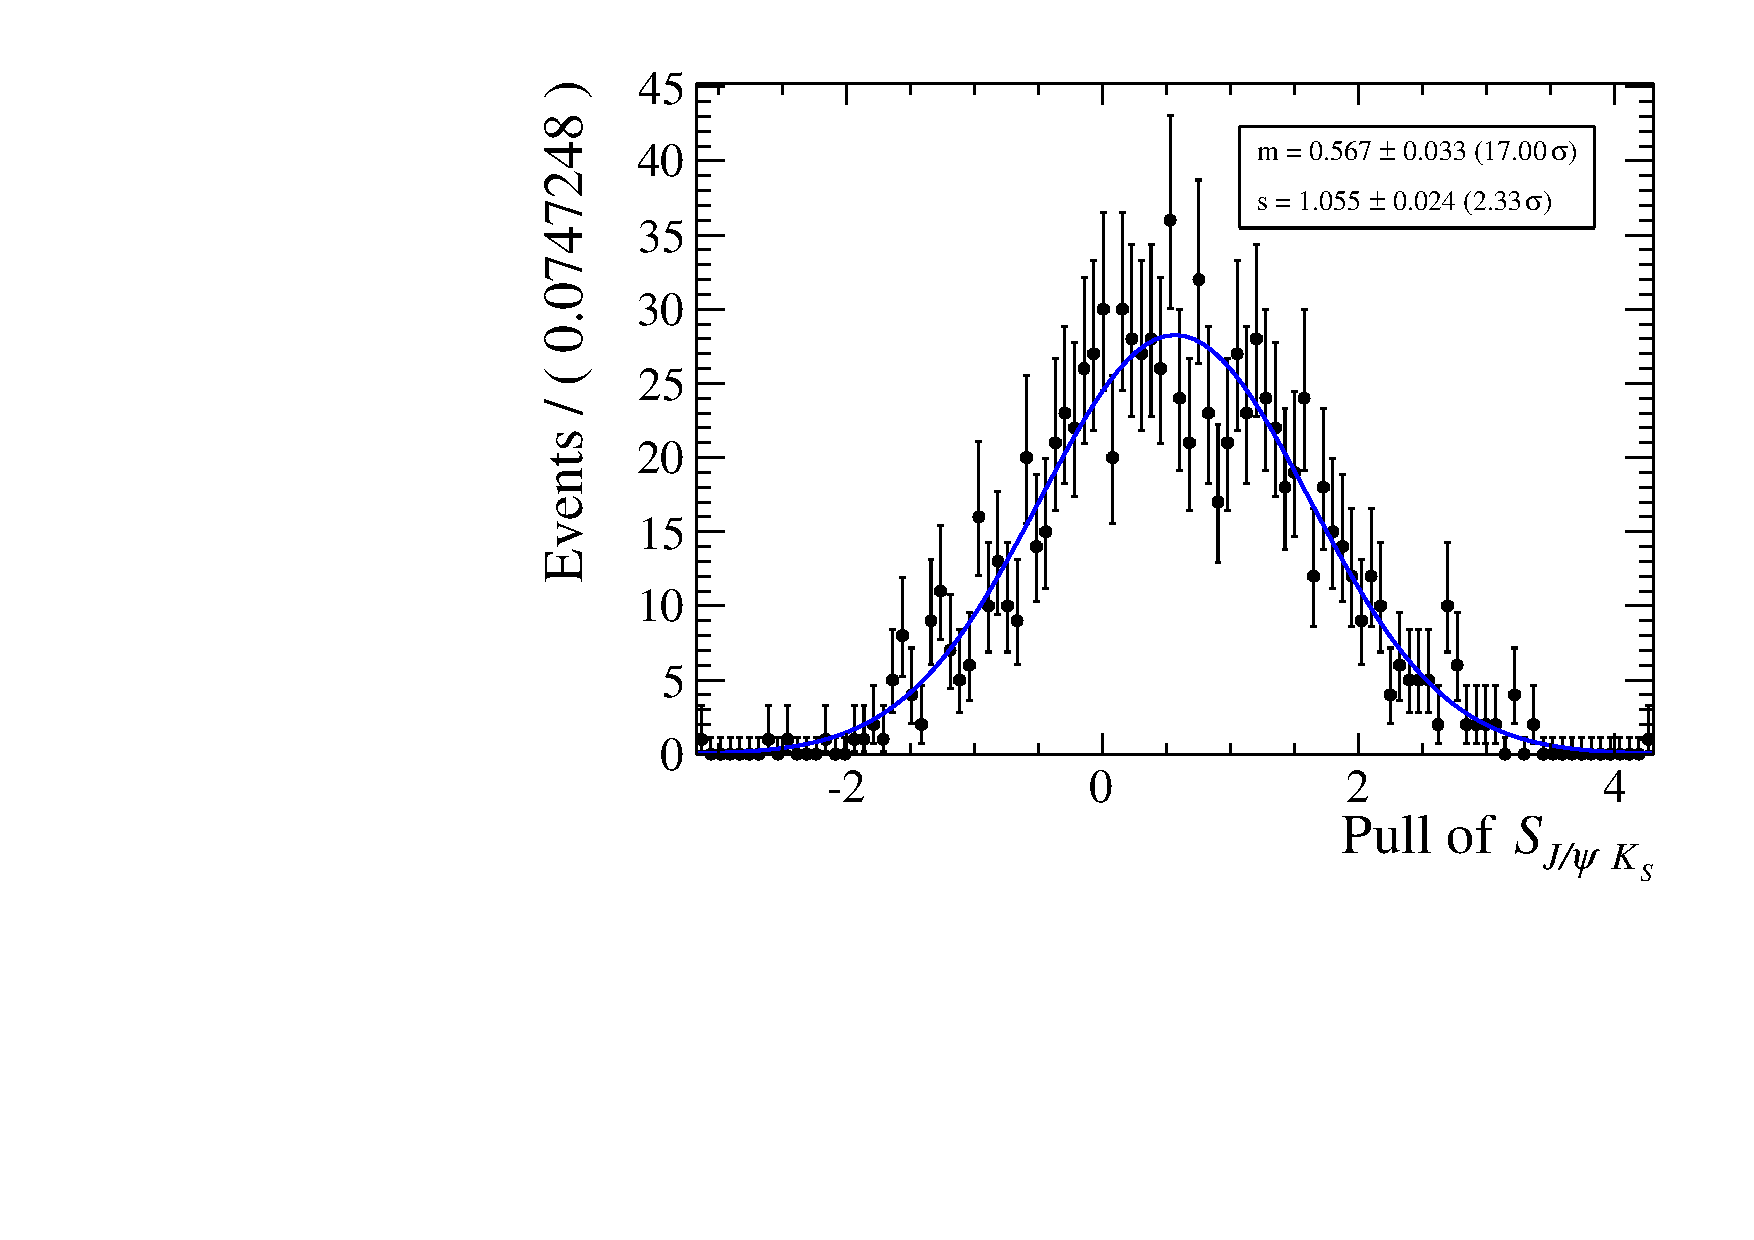
\includegraphics[width=0.49\textwidth]{private/content/appendices/figs/systematics_fitmodel_bkttaggingasym_s_pull.pdf}\hfill
  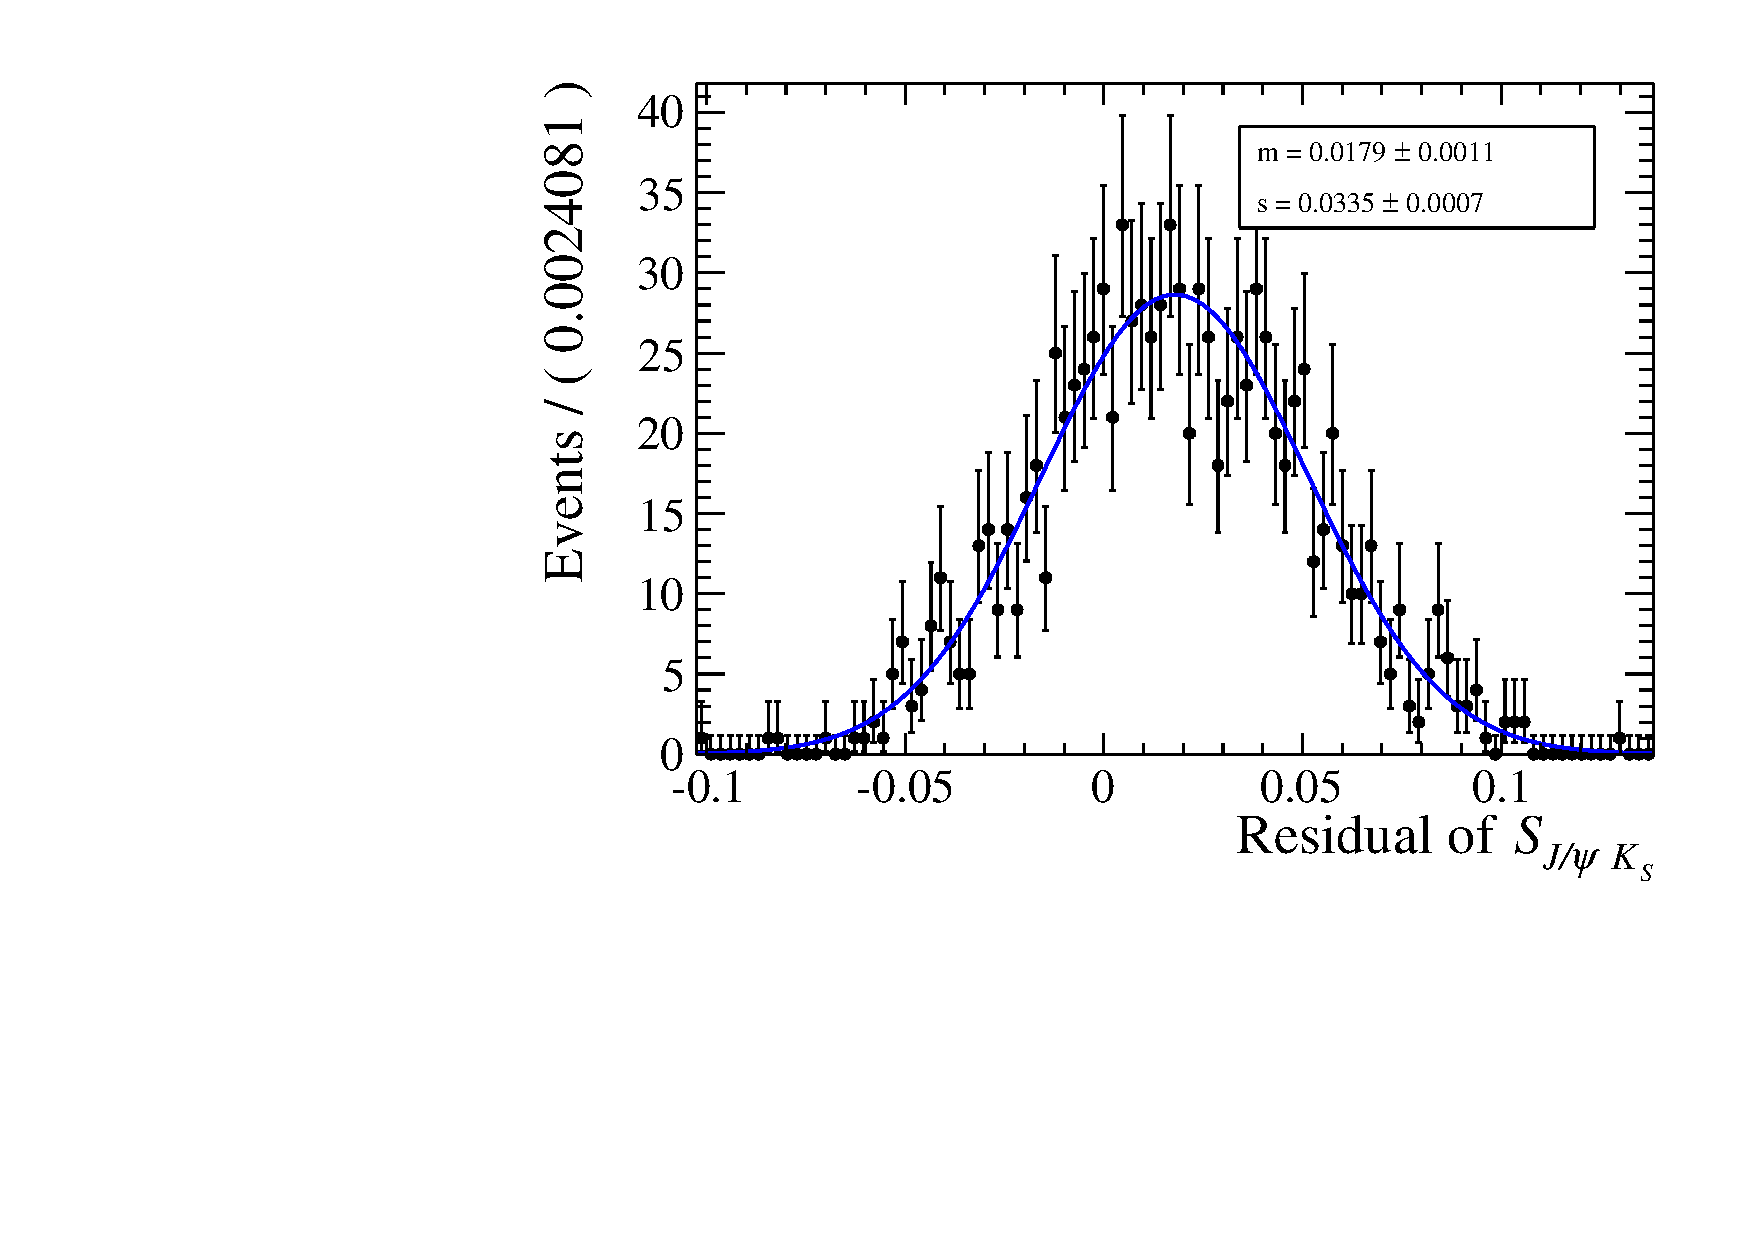
\includegraphics[width=0.49\textwidth]{private/content/appendices/figs/systematics_fitmodel_bkttaggingasym_s_res.pdf}\\
  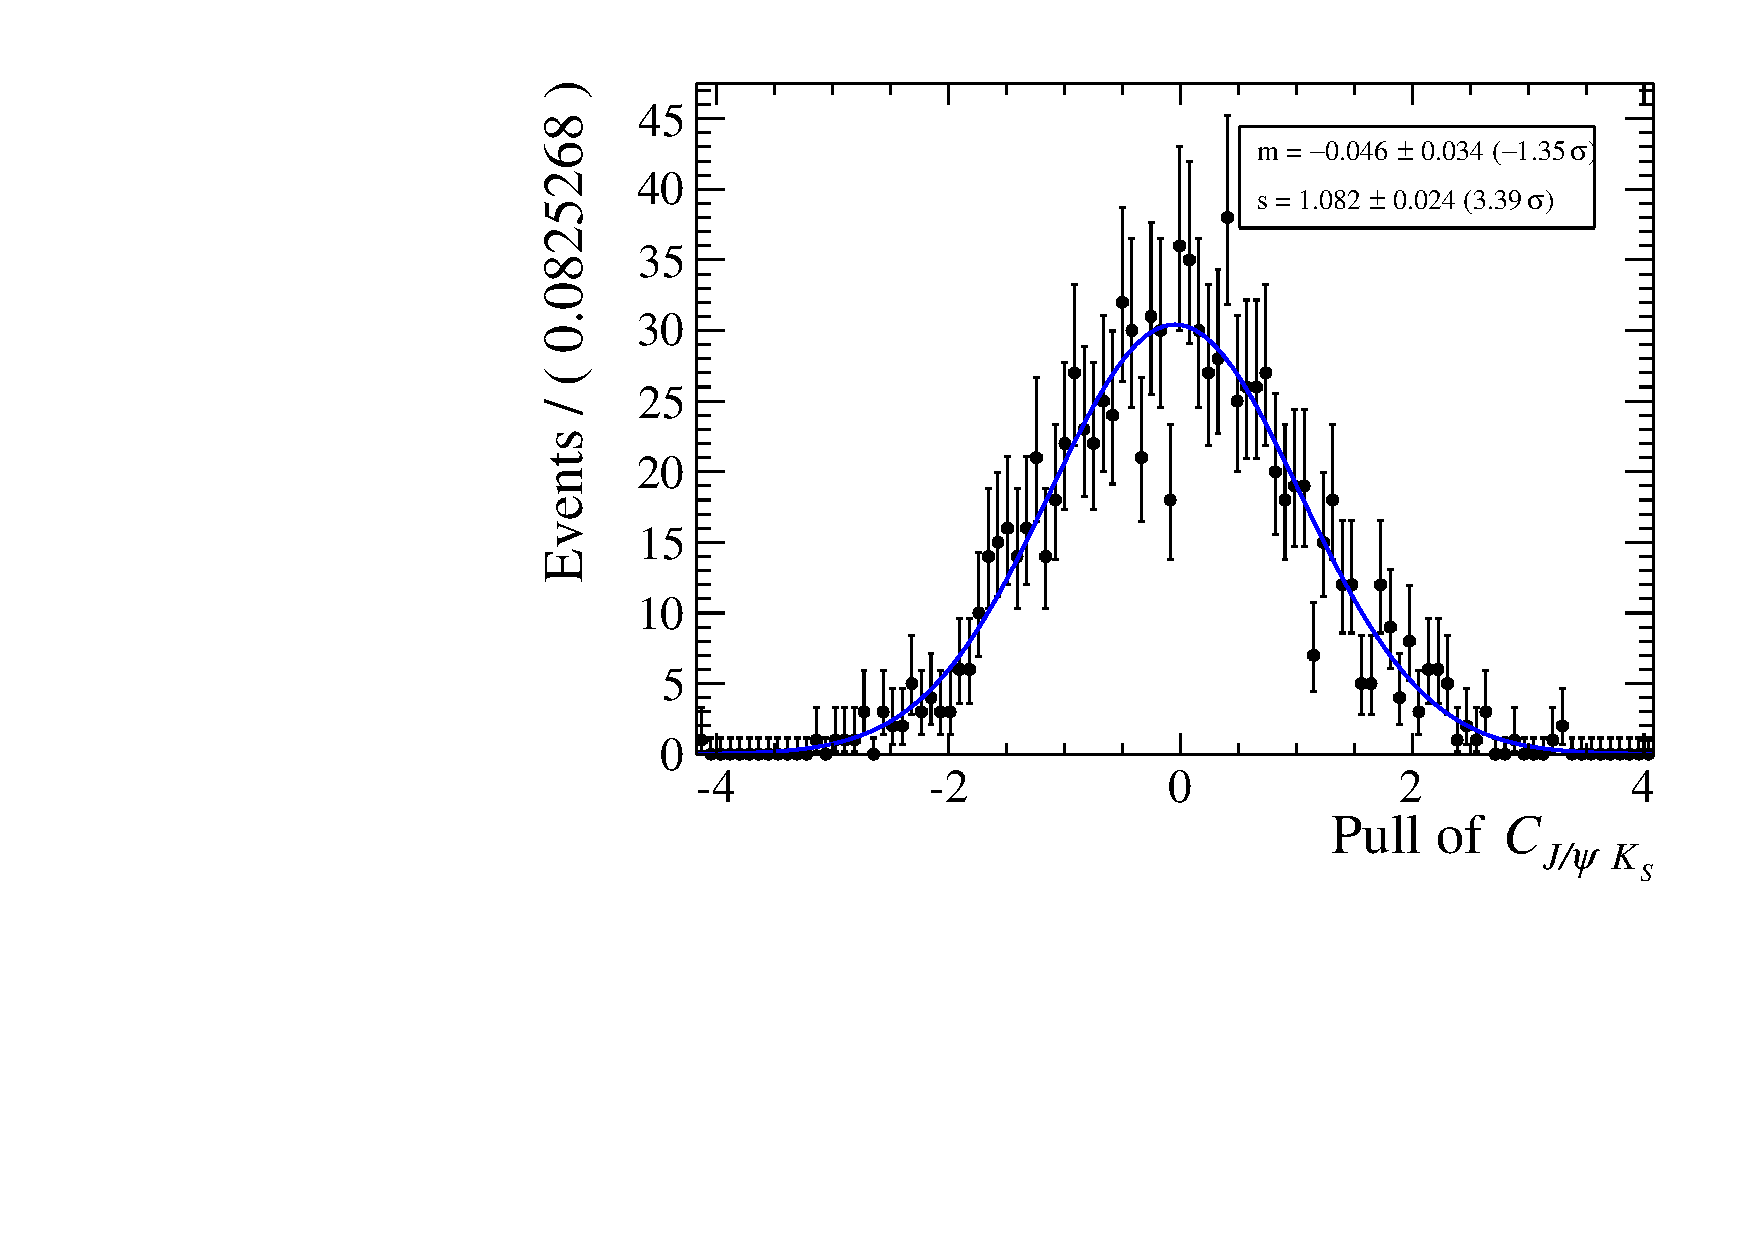
\includegraphics[width=0.49\textwidth]{private/content/appendices/figs/systematics_fitmodel_bkttaggingasym_c_pull.pdf}\hfill
  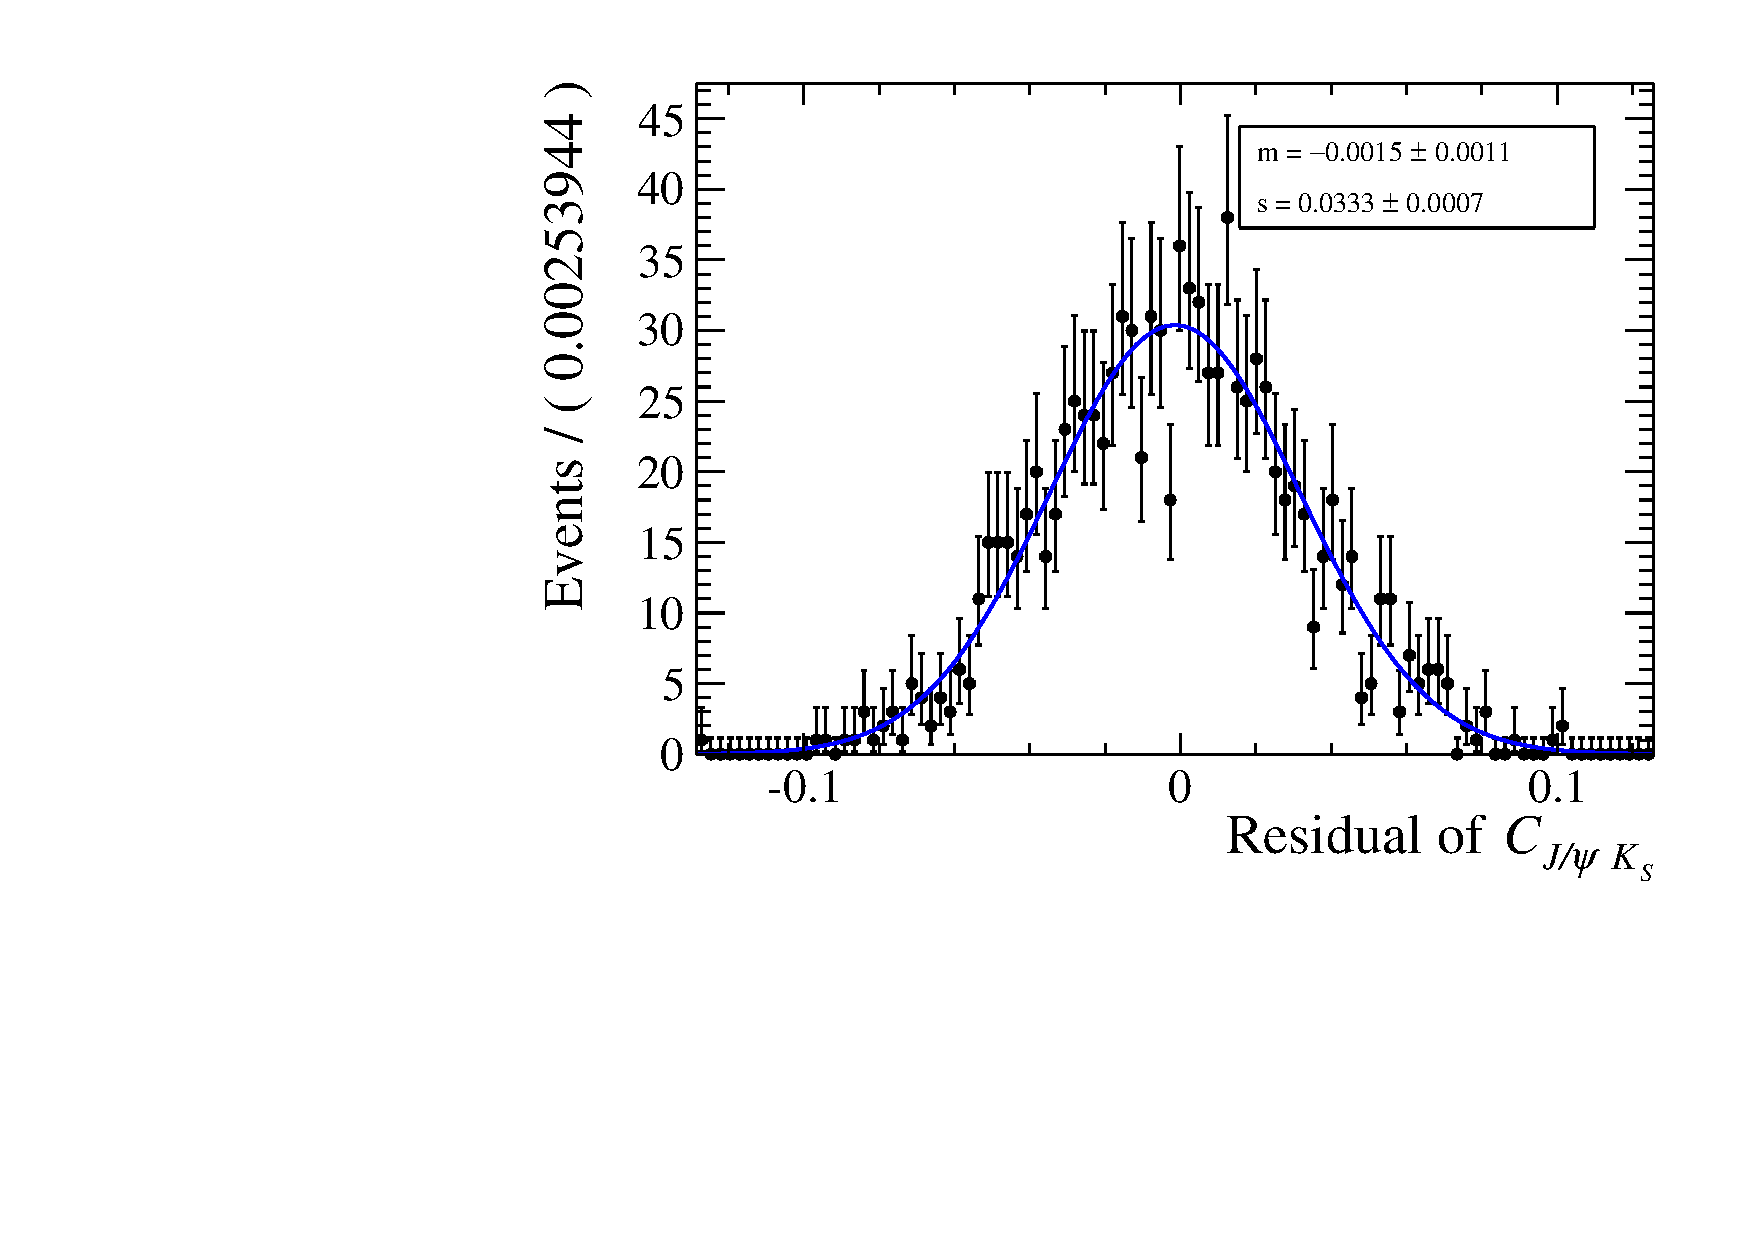
\includegraphics[width=0.49\textwidth]{private/content/appendices/figs/systematics_fitmodel_bkttaggingasym_c_res.pdf}
\caption{Shown are (left) pull and (right) residual distributions of the
parameters (top) \SJpsiKS and (bottom) \CJpsiKS from a \ToyMC study of the
influence of an asymmetry in the background tagging estimates on the measurement
of the \CP parameters.}
\label{fig:app:measurement_of_sin2beta:systematics:systematics:fit_model:bkg_tagging_asymmetry}
\end{figure}

\begin{figure}[h]
\centering
  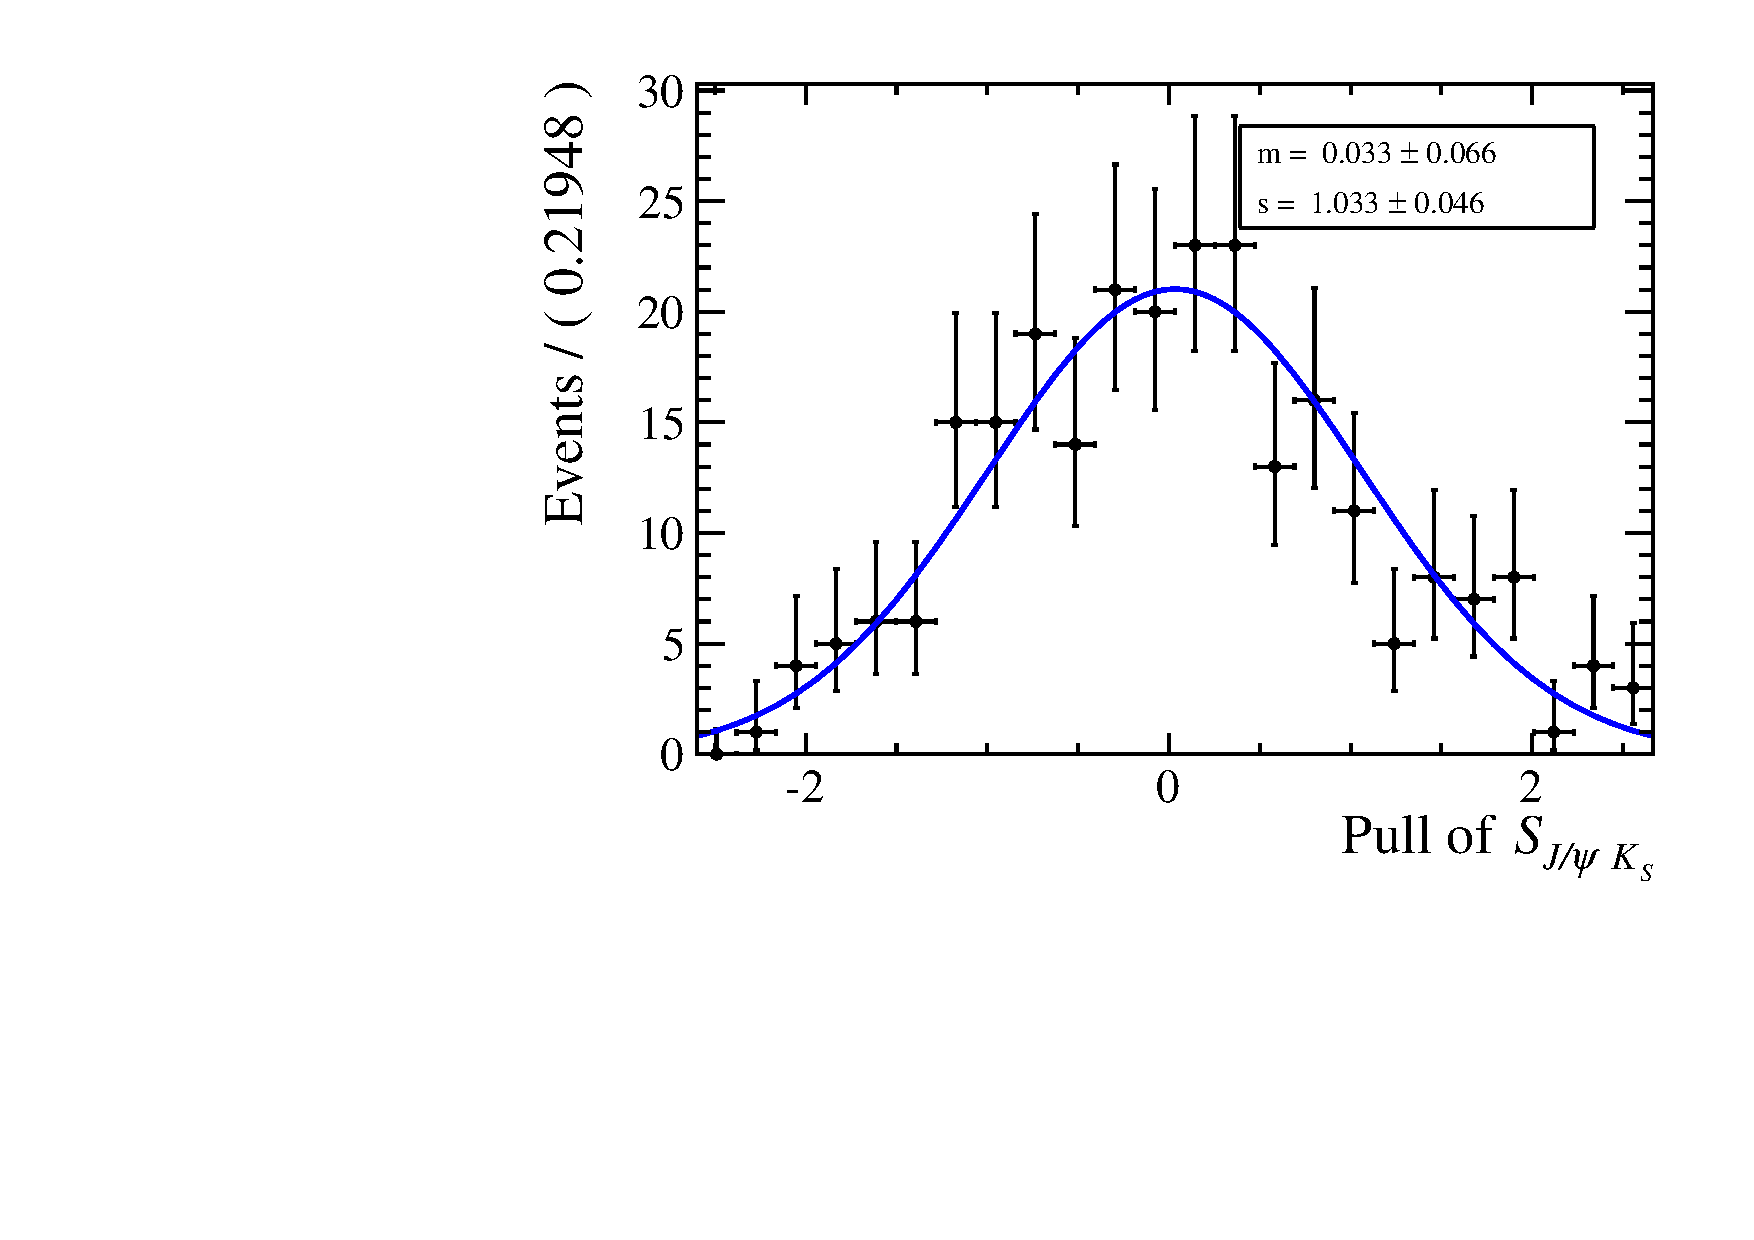
\includegraphics[width=0.49\textwidth]{private/content/appendices/figs/systematics_fitmodel_mtcorr_s_pull.pdf}\hfill
  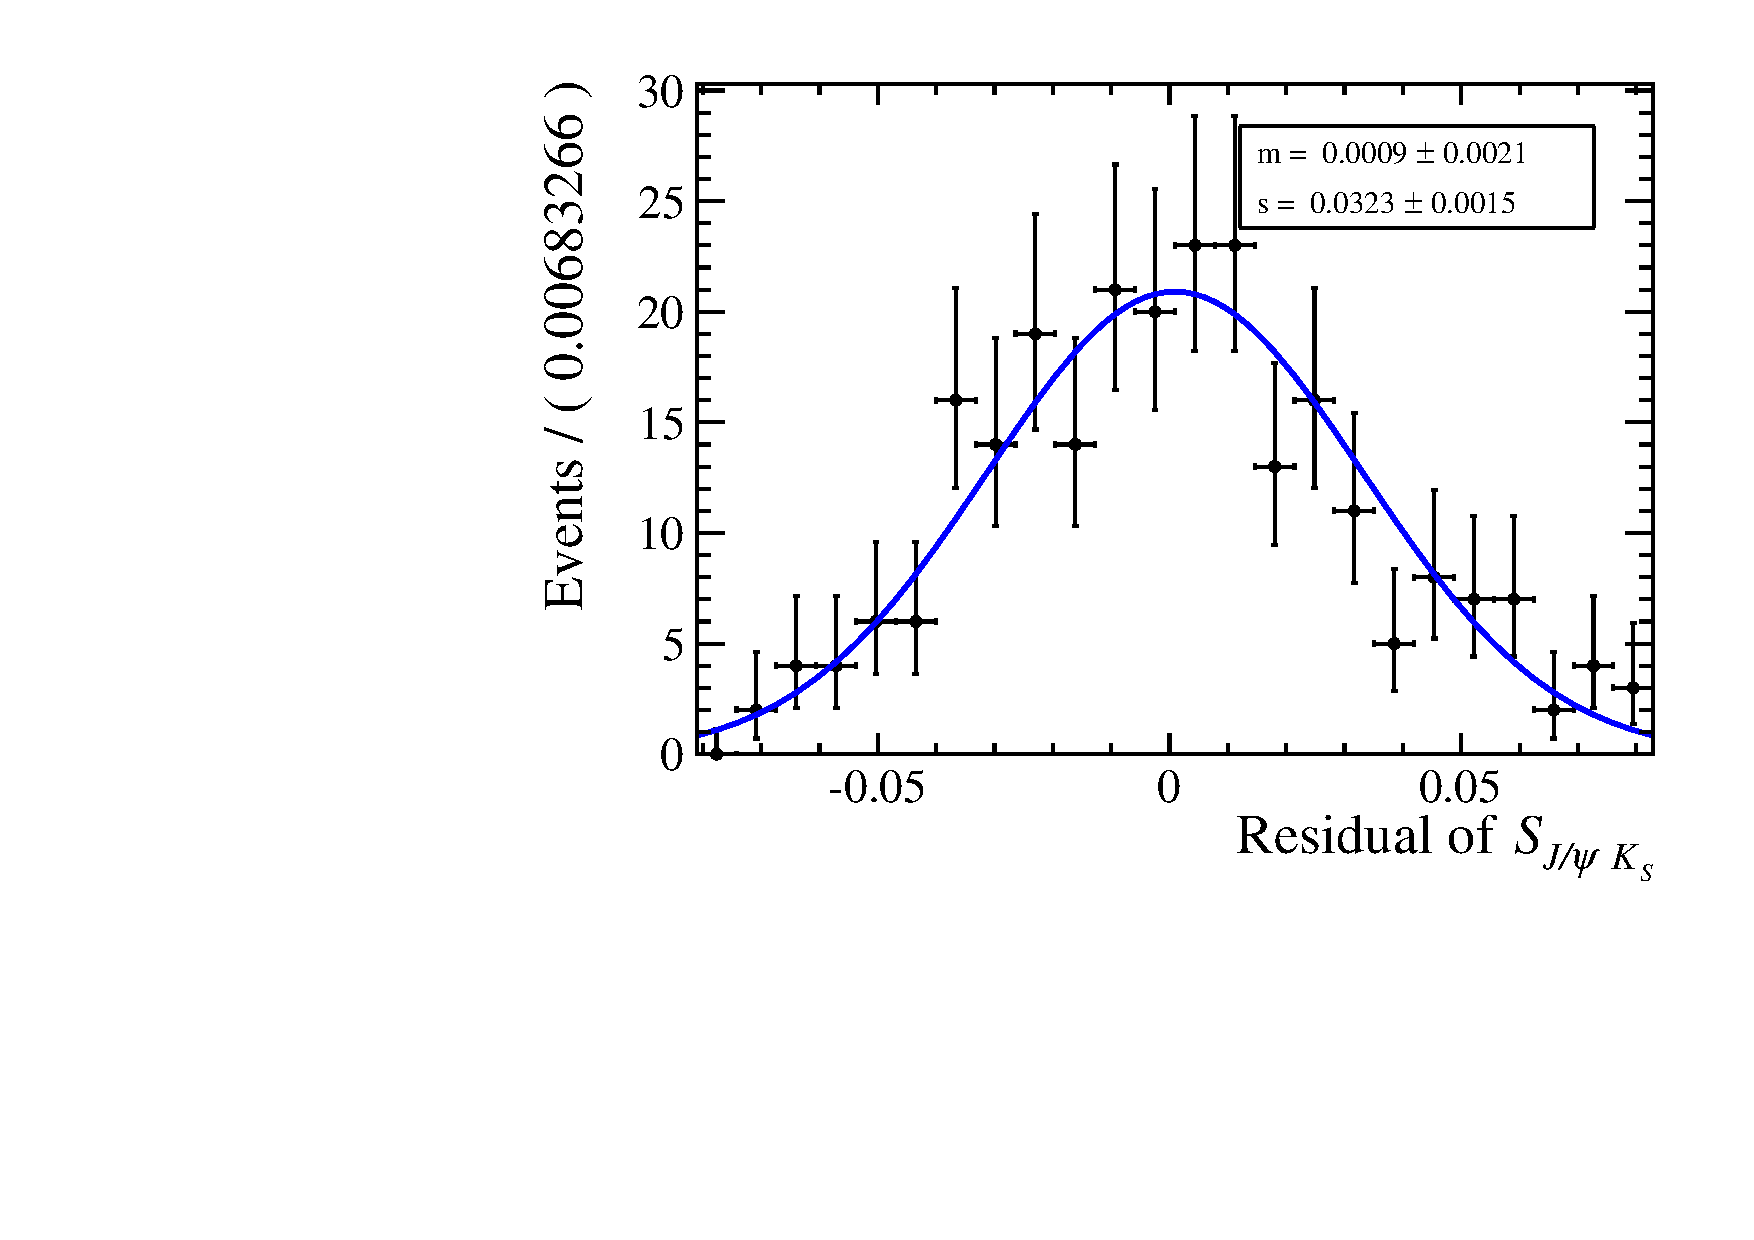
\includegraphics[width=0.49\textwidth]{private/content/appendices/figs/systematics_fitmodel_mtcorr_s_res.pdf}\\
  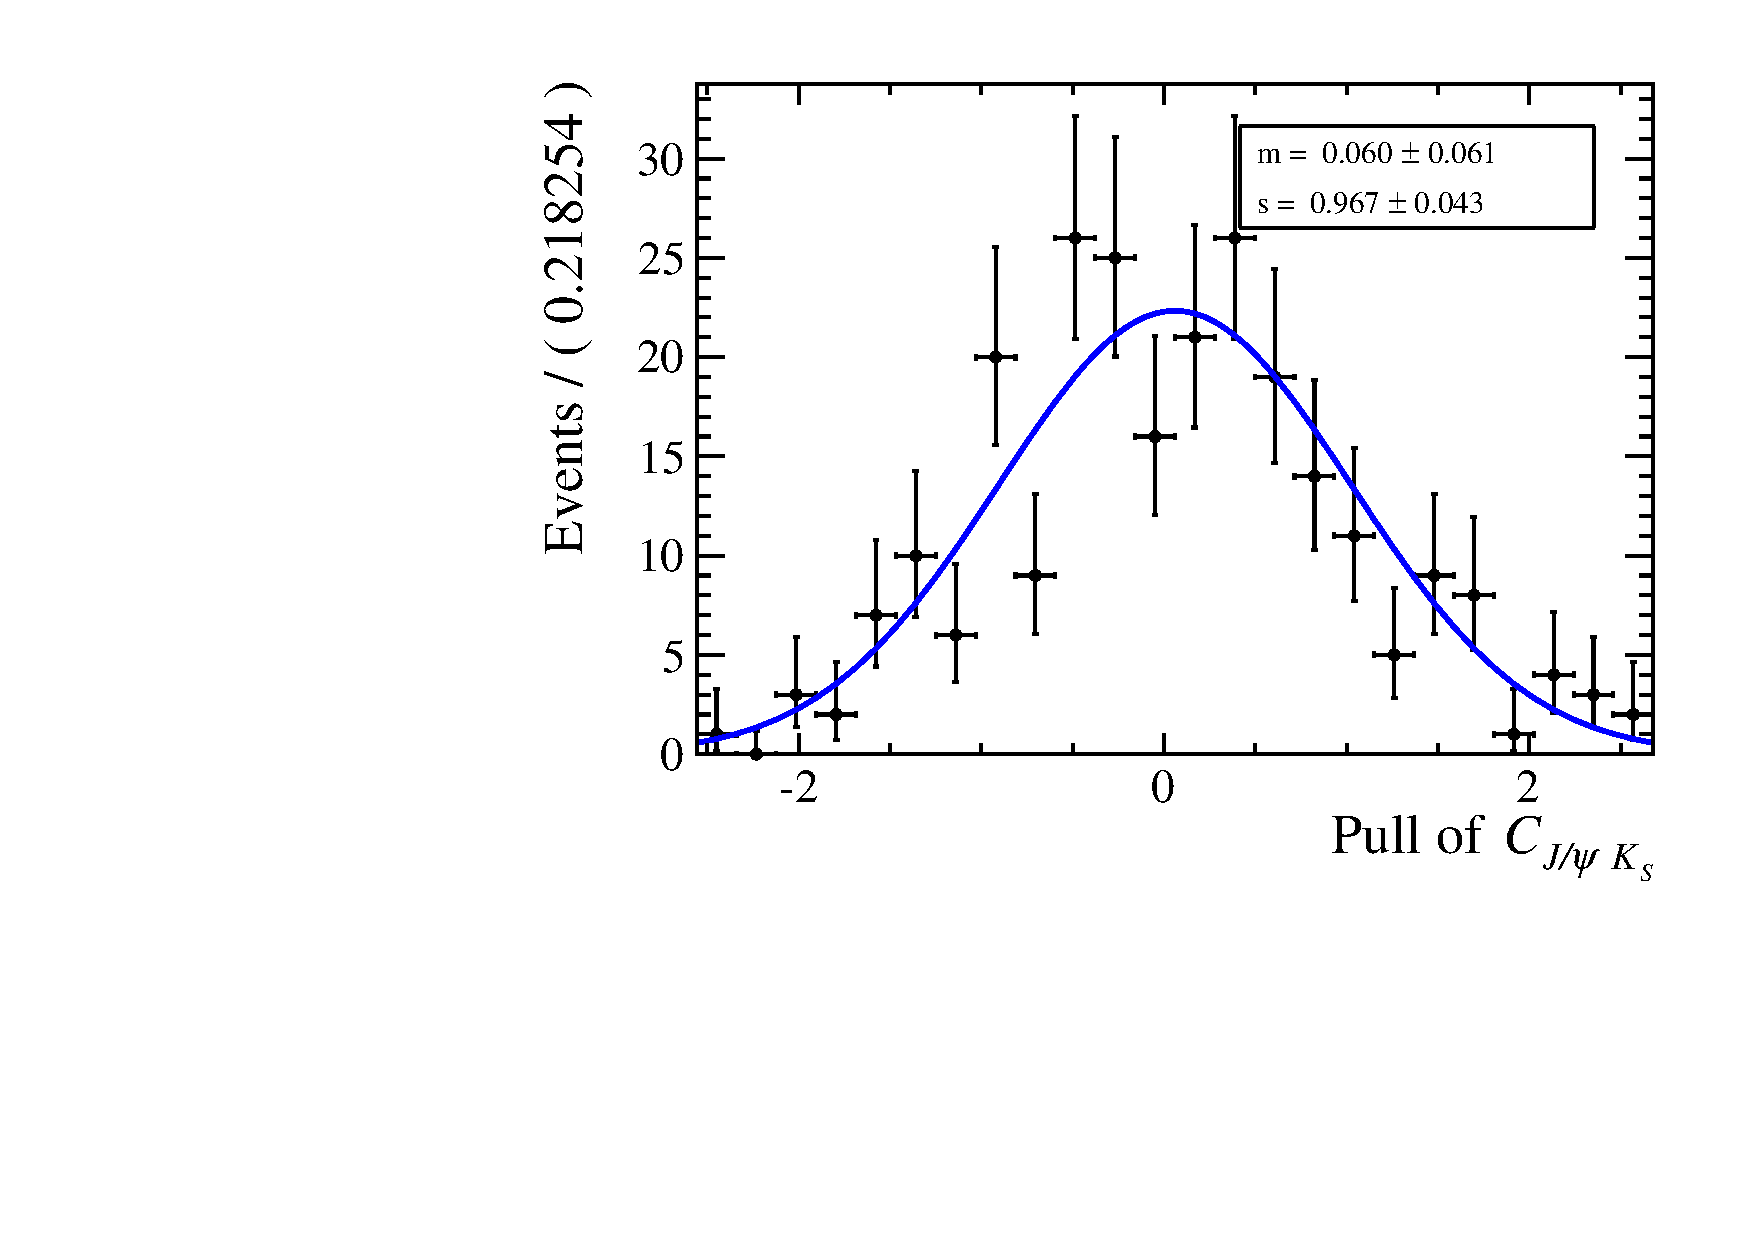
\includegraphics[width=0.49\textwidth]{private/content/appendices/figs/systematics_fitmodel_mtcorr_c_pull.pdf}\hfill
  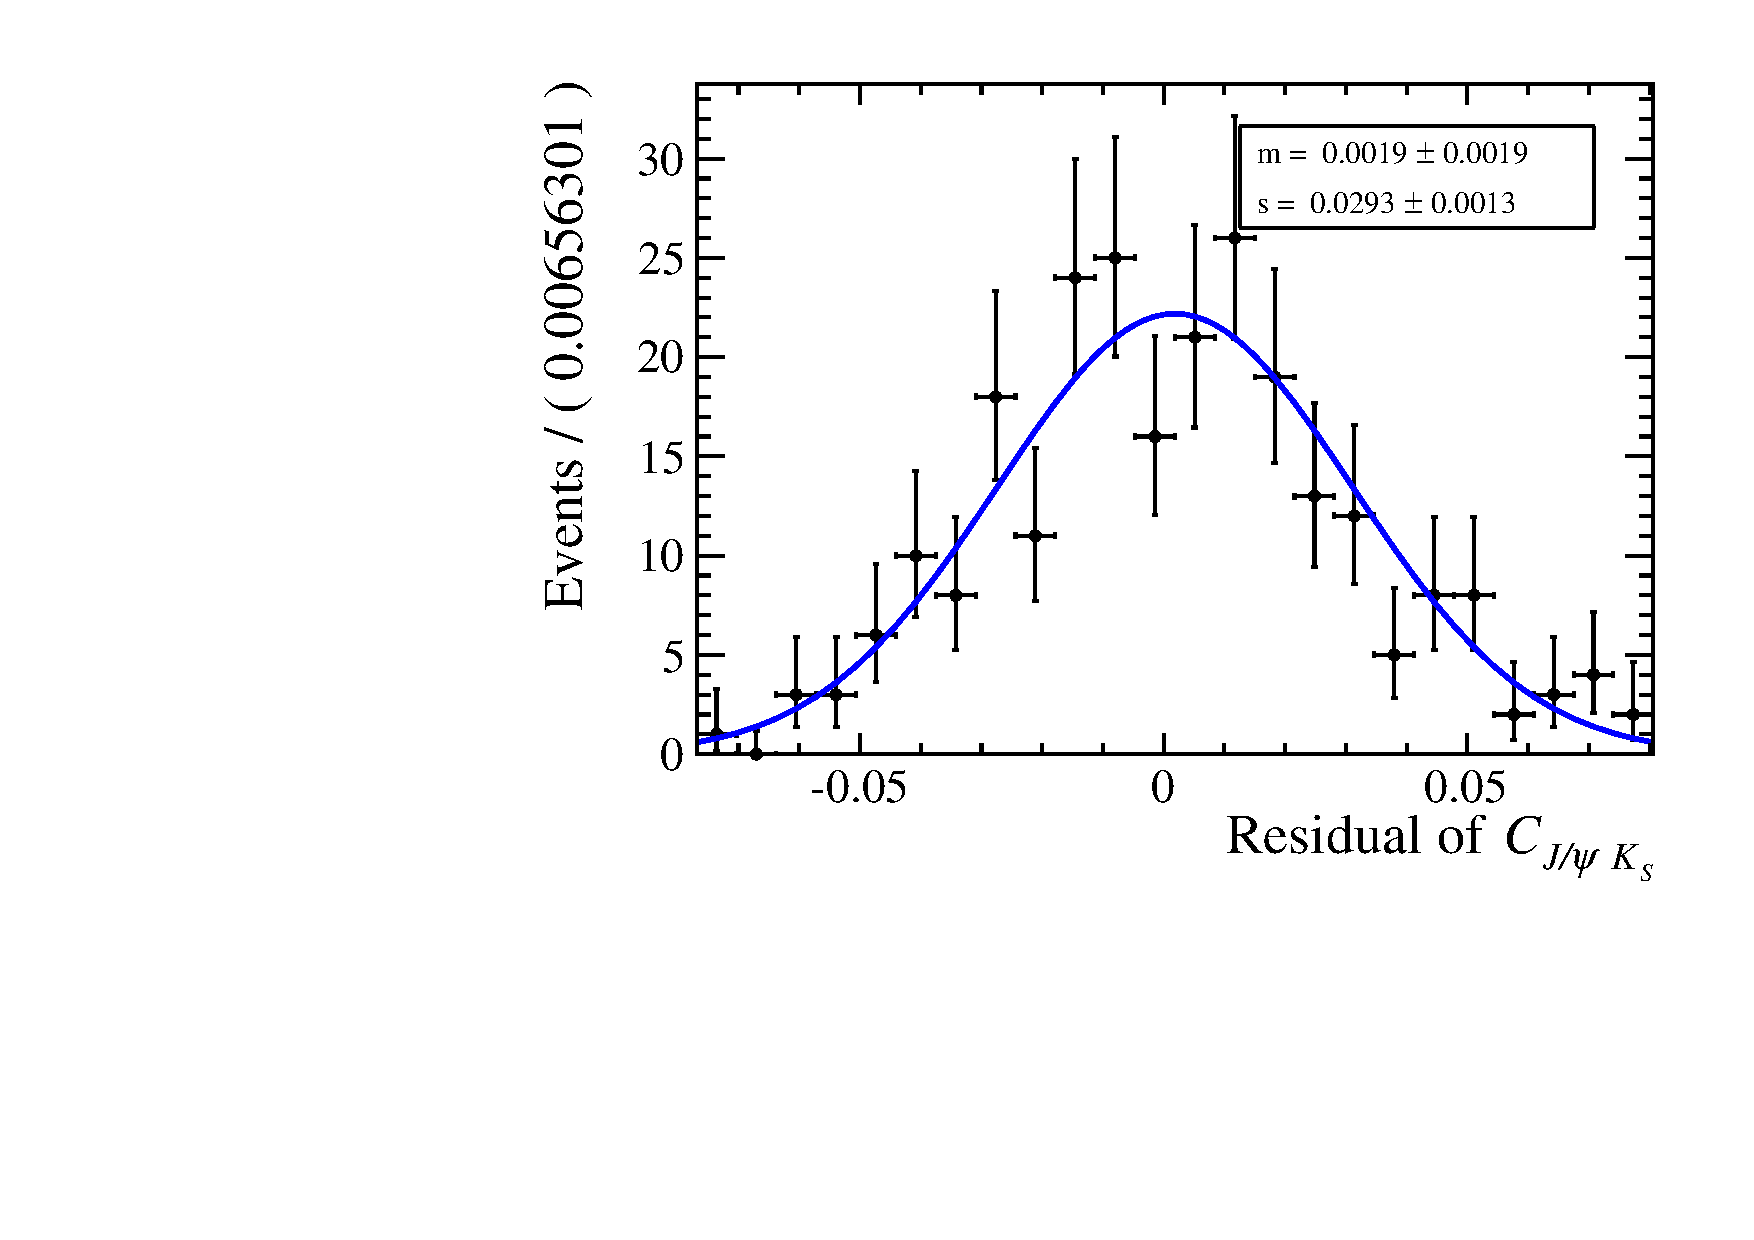
\includegraphics[width=0.49\textwidth]{private/content/appendices/figs/systematics_fitmodel_mtcorr_c_res.pdf}
\caption{Shown are (left) pull and (right) residual distributions of the
parameters (top) \SJpsiKS and (bottom) \CJpsiKS from a \ToyMC study of the
influence of a small mass and decay time correlation on the measurement of the
\CP parameters.}
\label{fig:app:measurement_of_sin2beta:systematics:systematics:fit_model:mass_time_correlations}
\end{figure}

\clearpage
% ..............................................................................
\subsubsection{Flavour Tagging}
\label{sec:app:measurement_of_sin2beta:systematics:systematics:tagging}

\begin{figure}[h]
  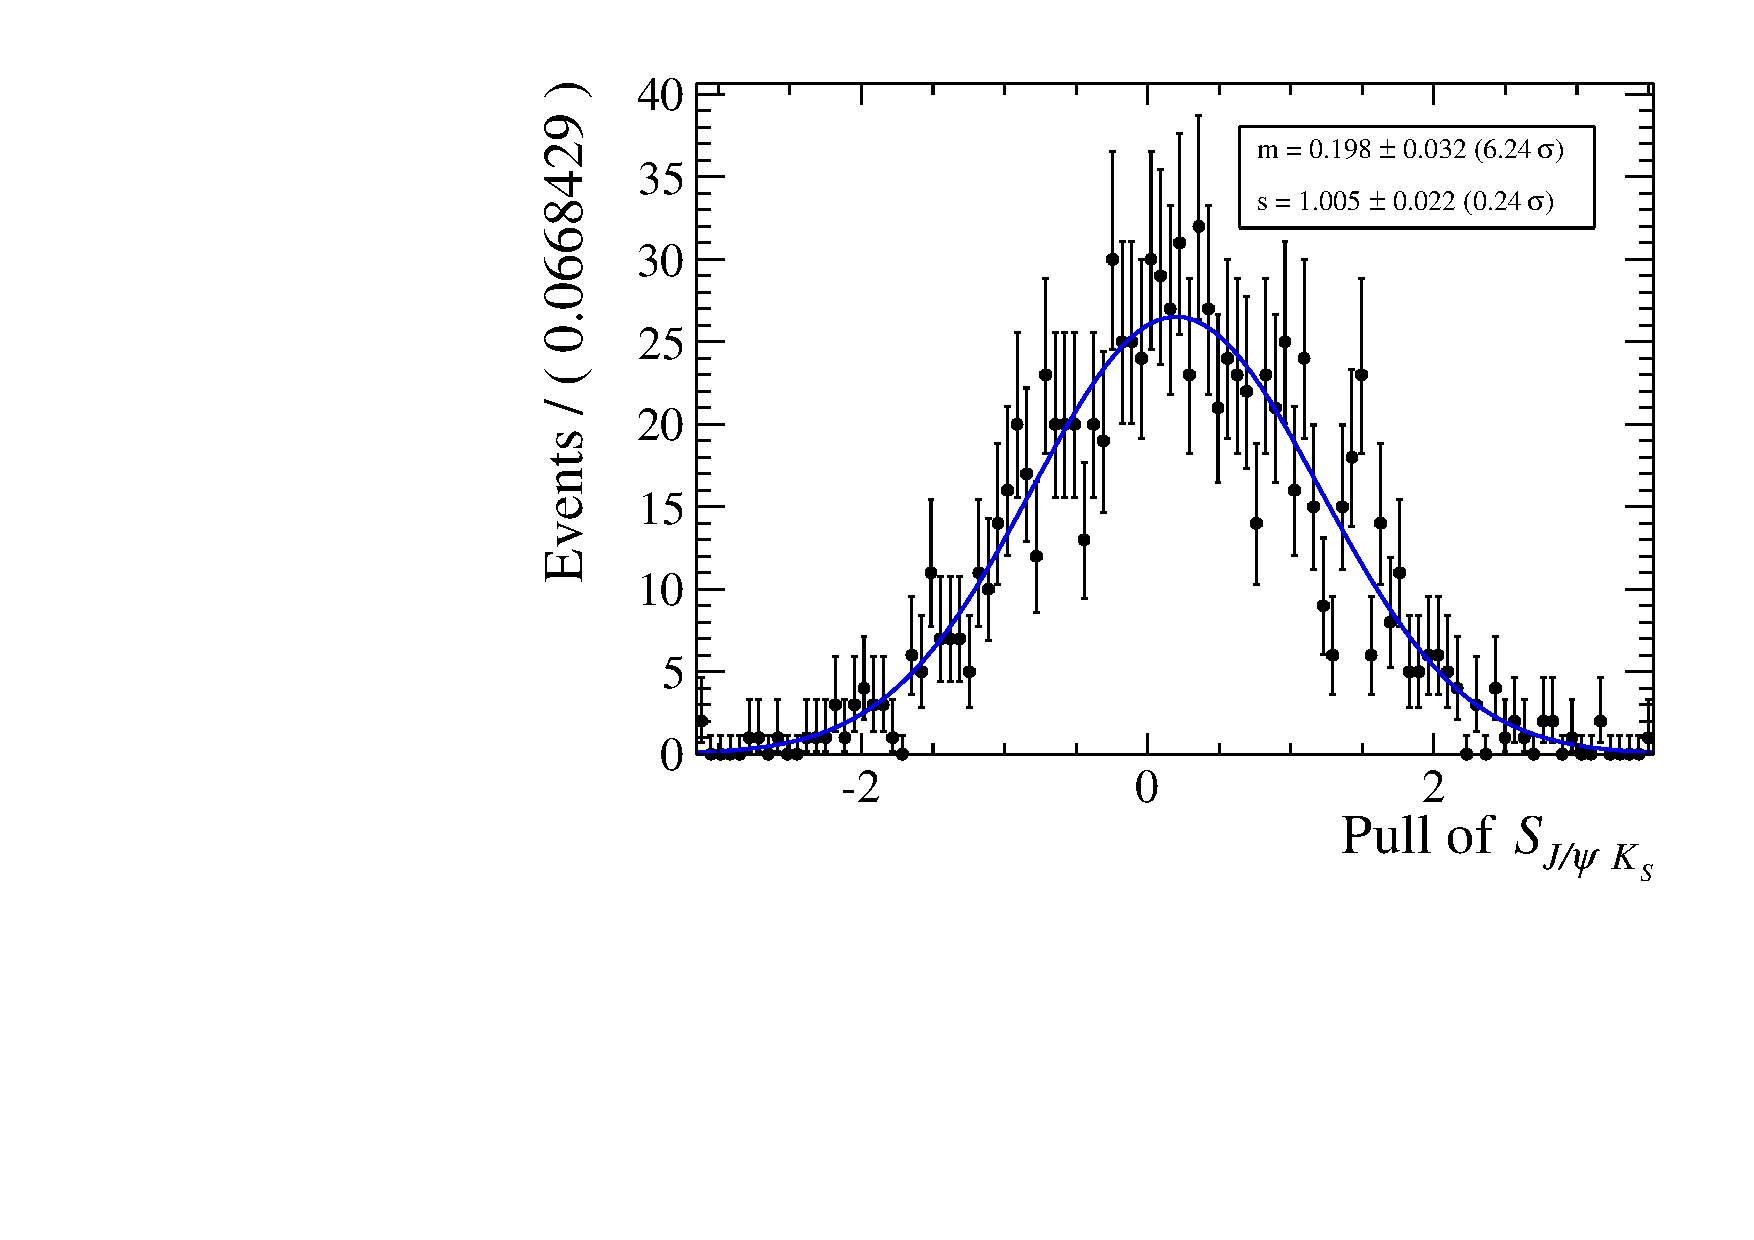
\includegraphics[width=0.49\textwidth]{private/content/appendices/figs/systematics_ft_calibration_s_pull.pdf}\hfill
  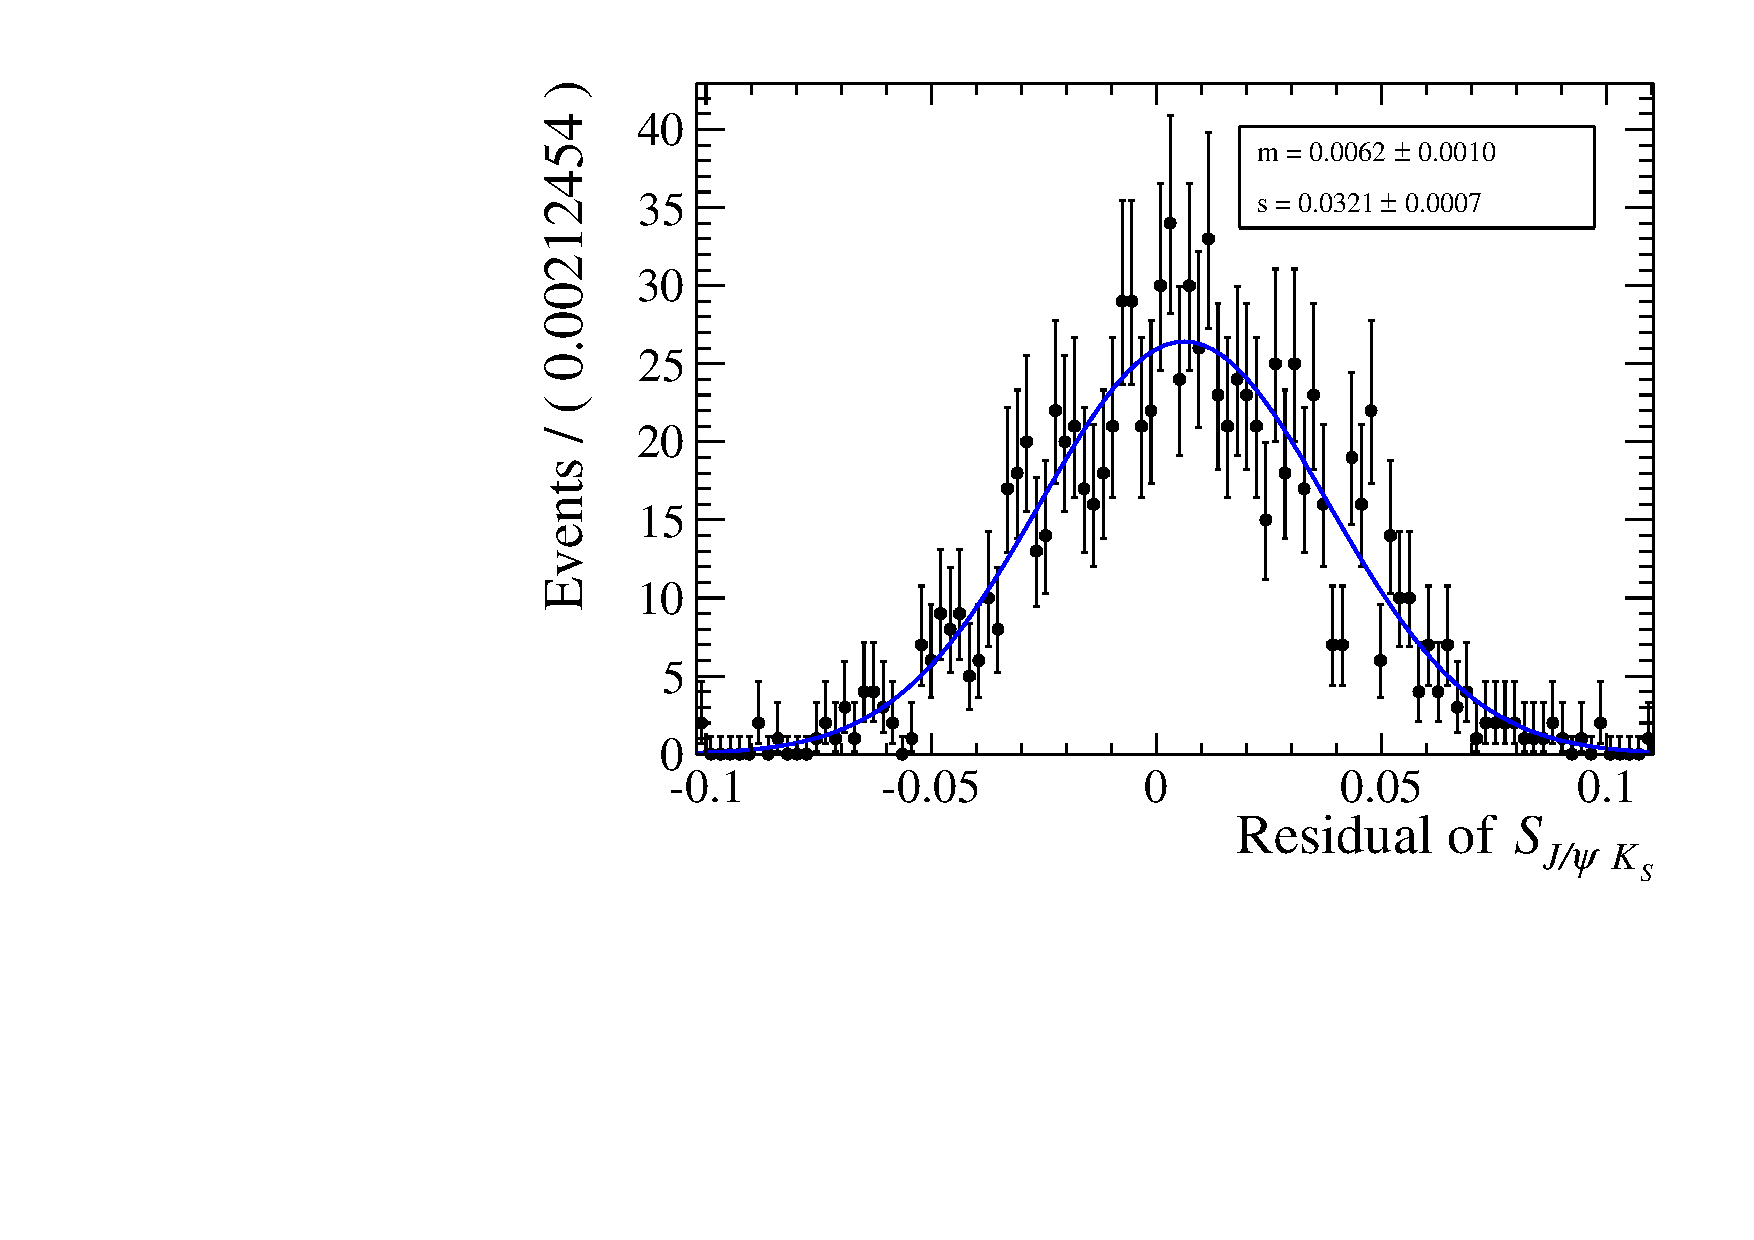
\includegraphics[width=0.49\textwidth]{private/content/appendices/figs/systematics_ft_calibration_s_res.pdf}
  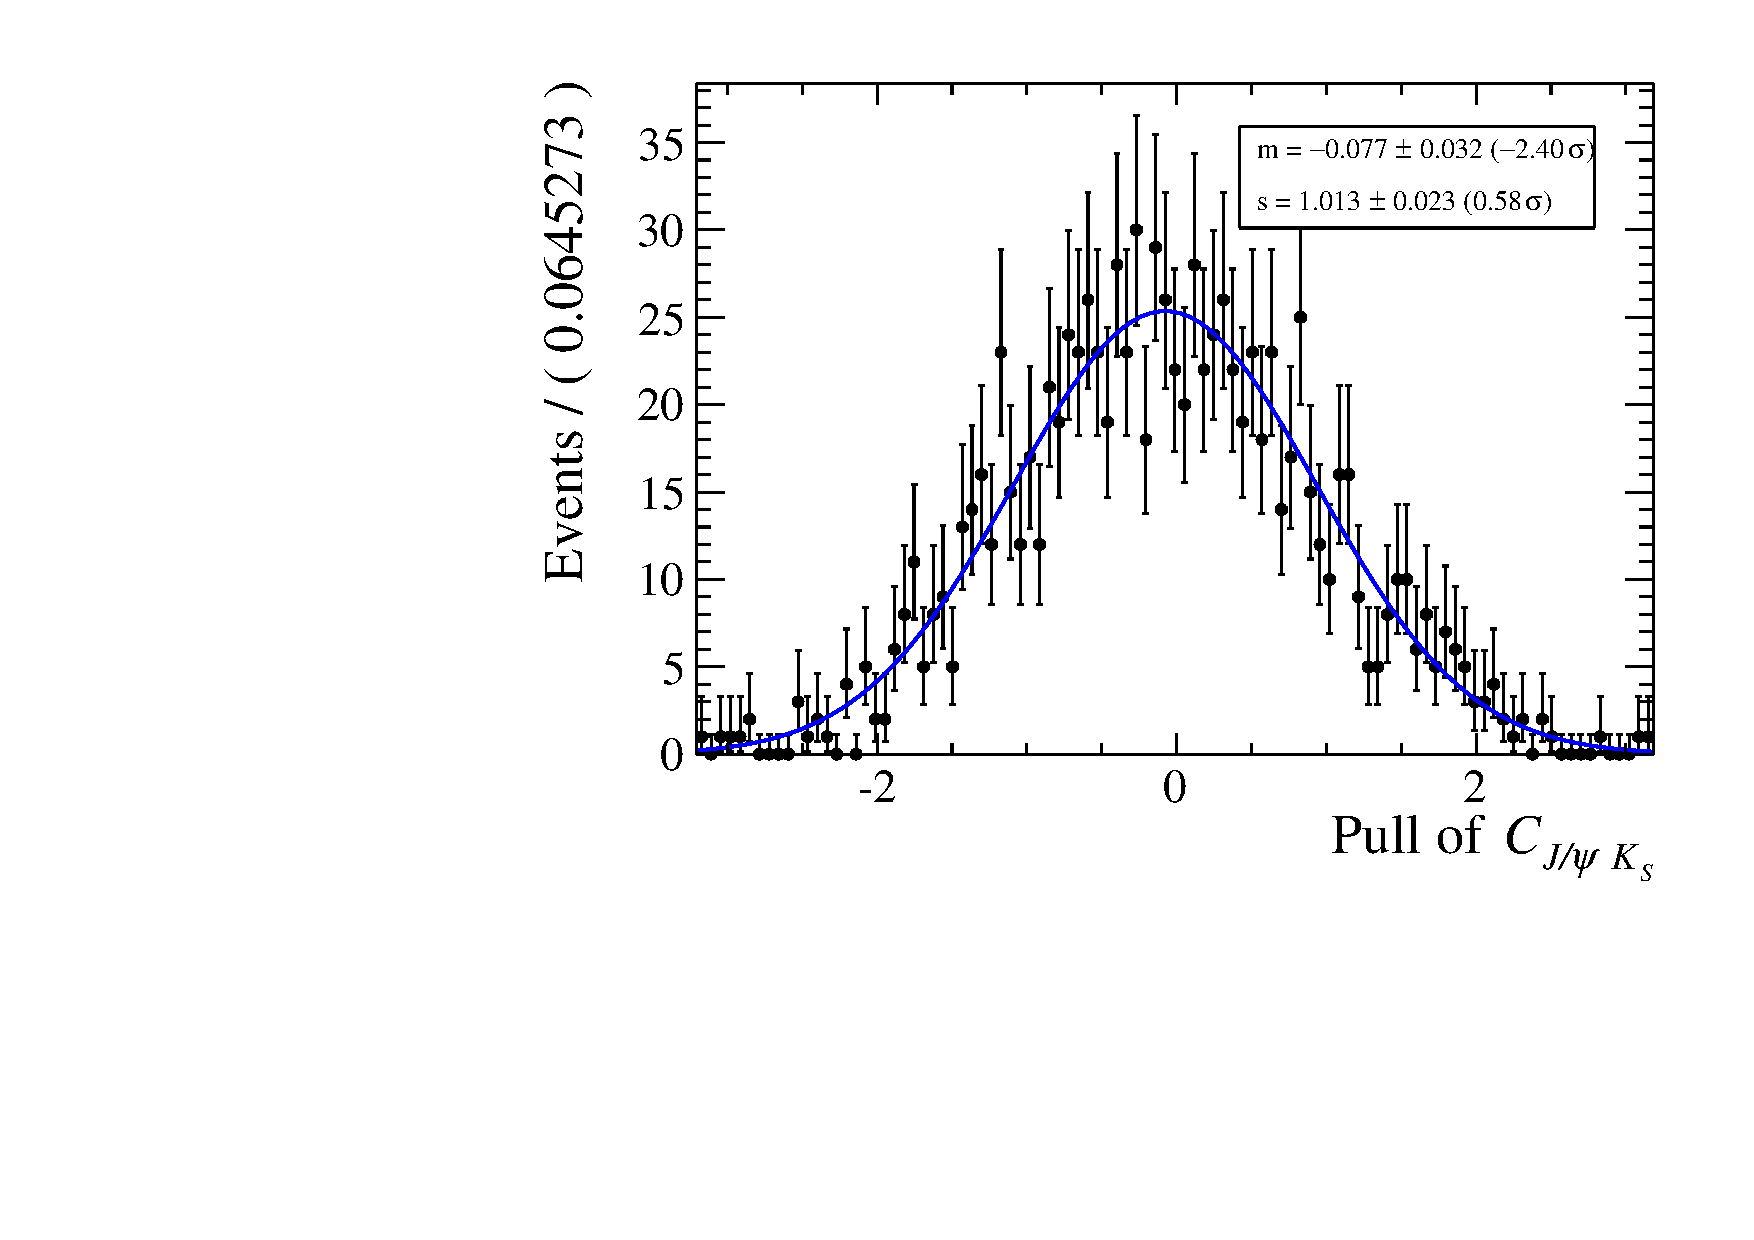
\includegraphics[width=0.49\textwidth]{private/content/appendices/figs/systematics_ft_calibration_c_pull.pdf}\hfill
  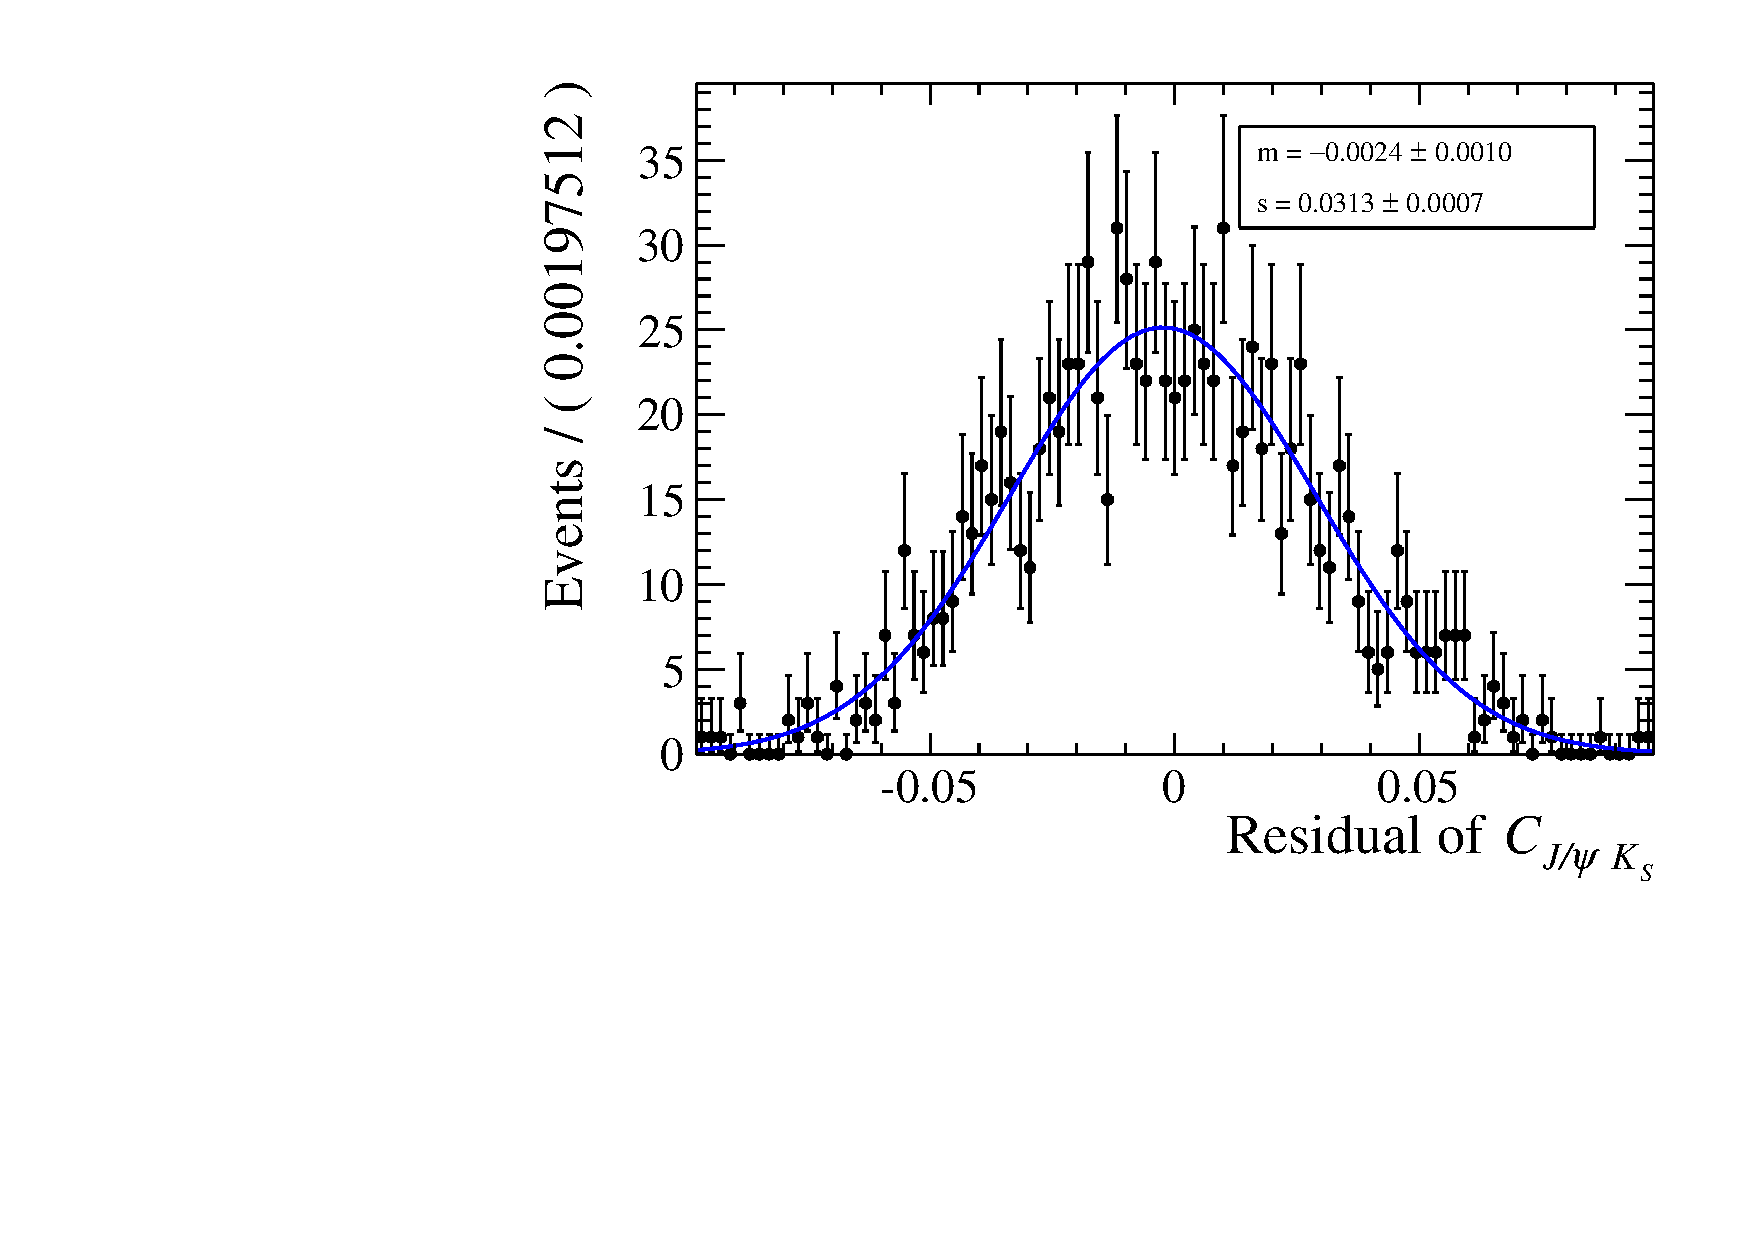
\includegraphics[width=0.49\textwidth]{private/content/appendices/figs/systematics_ft_calibration_c_res.pdf}
\caption{Shown are (left) pull and (right) residual distributions of the
parameters (top) \SJpsiKS and (bottom) \CJpsiKS from a \ToyMC study of the
influence of the systematic uncertainties on the flavour tagging calibration
parameters on the measurement of the \CP parameters.}
\label{fig:app:measurement_of_sin2beta:systematics:systematics:tagging}
\end{figure}

\clearpage
% ..............................................................................
\subsubsection{Decay time resolution}
\label{sec:app:measurement_of_sin2beta:systematics:systematics:resolution}

\begin{figure}[h]
  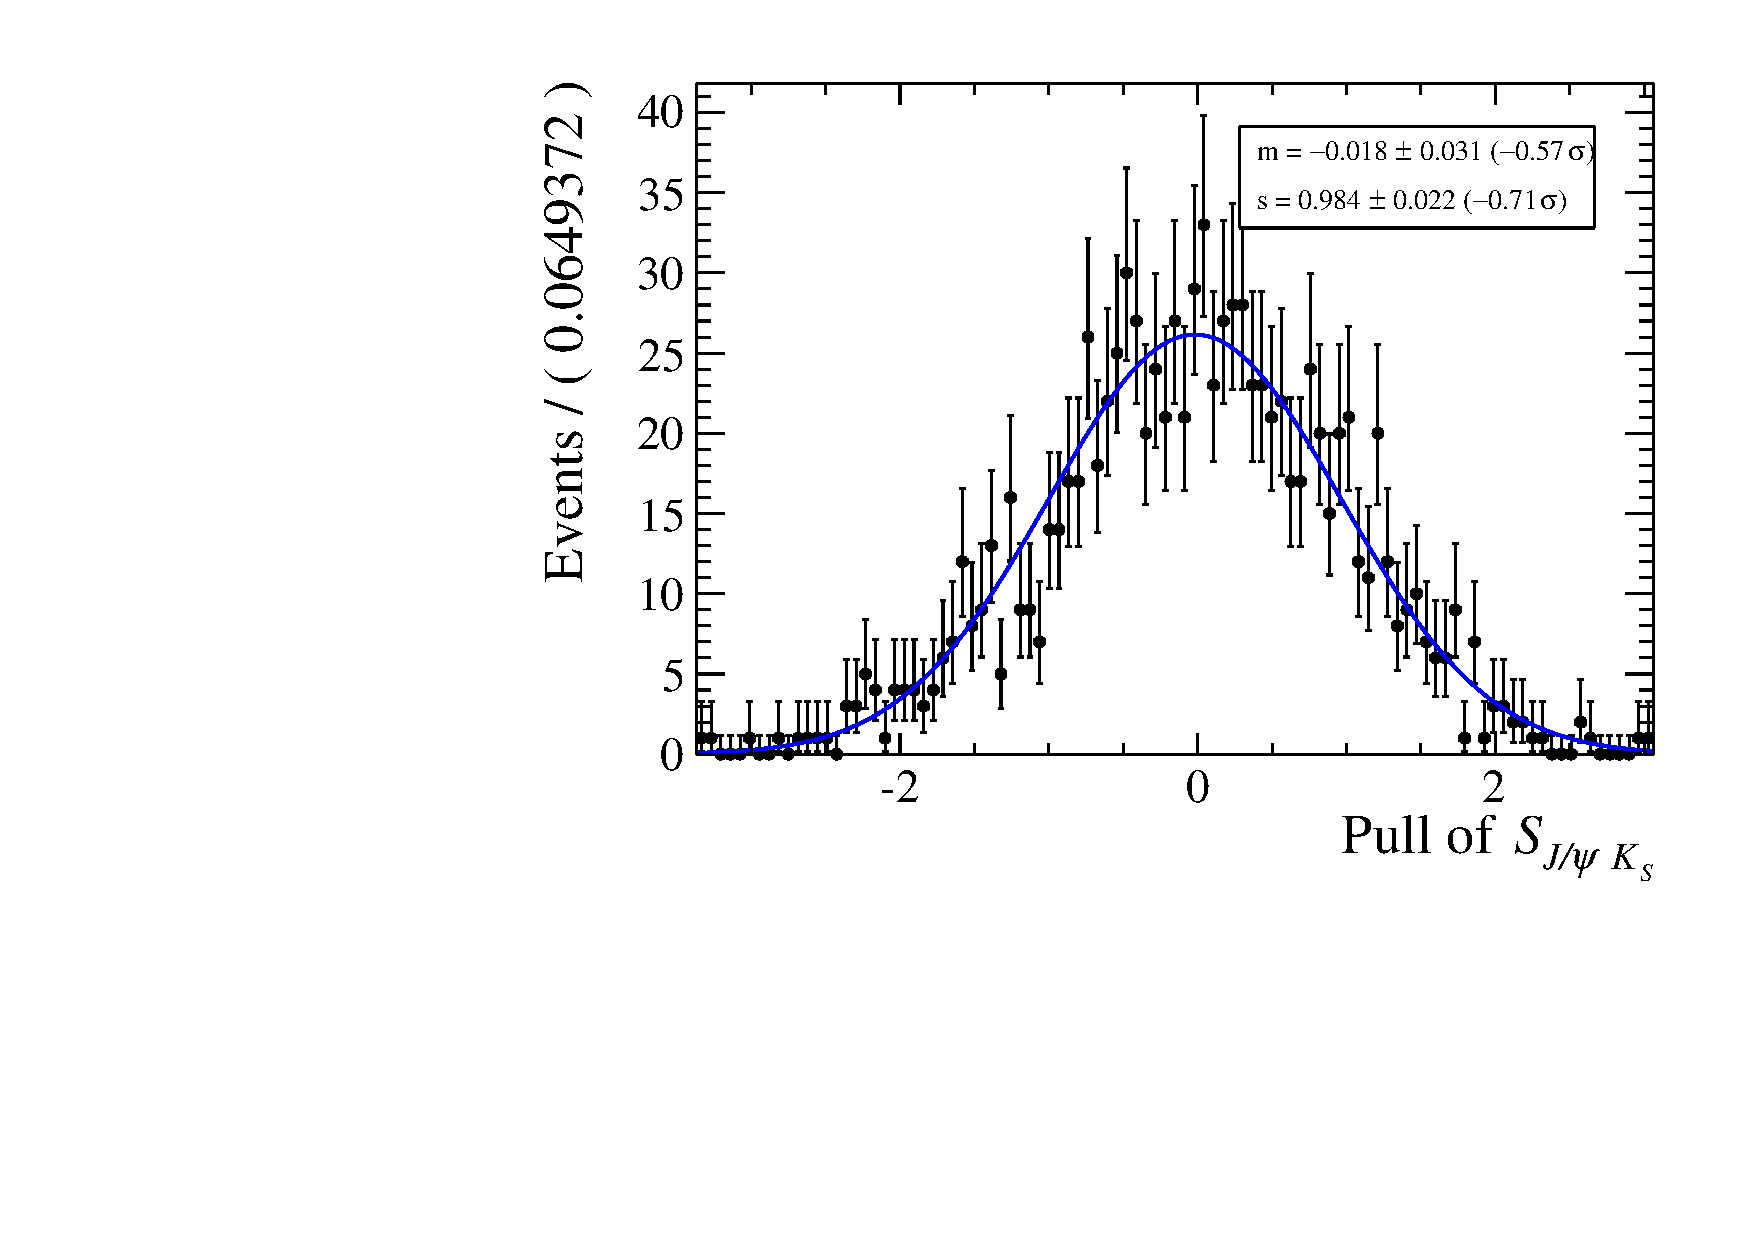
\includegraphics[width=0.49\textwidth]{private/content/appendices/figs/systematics_resolution_calibration_s_pull.pdf}\hfill
  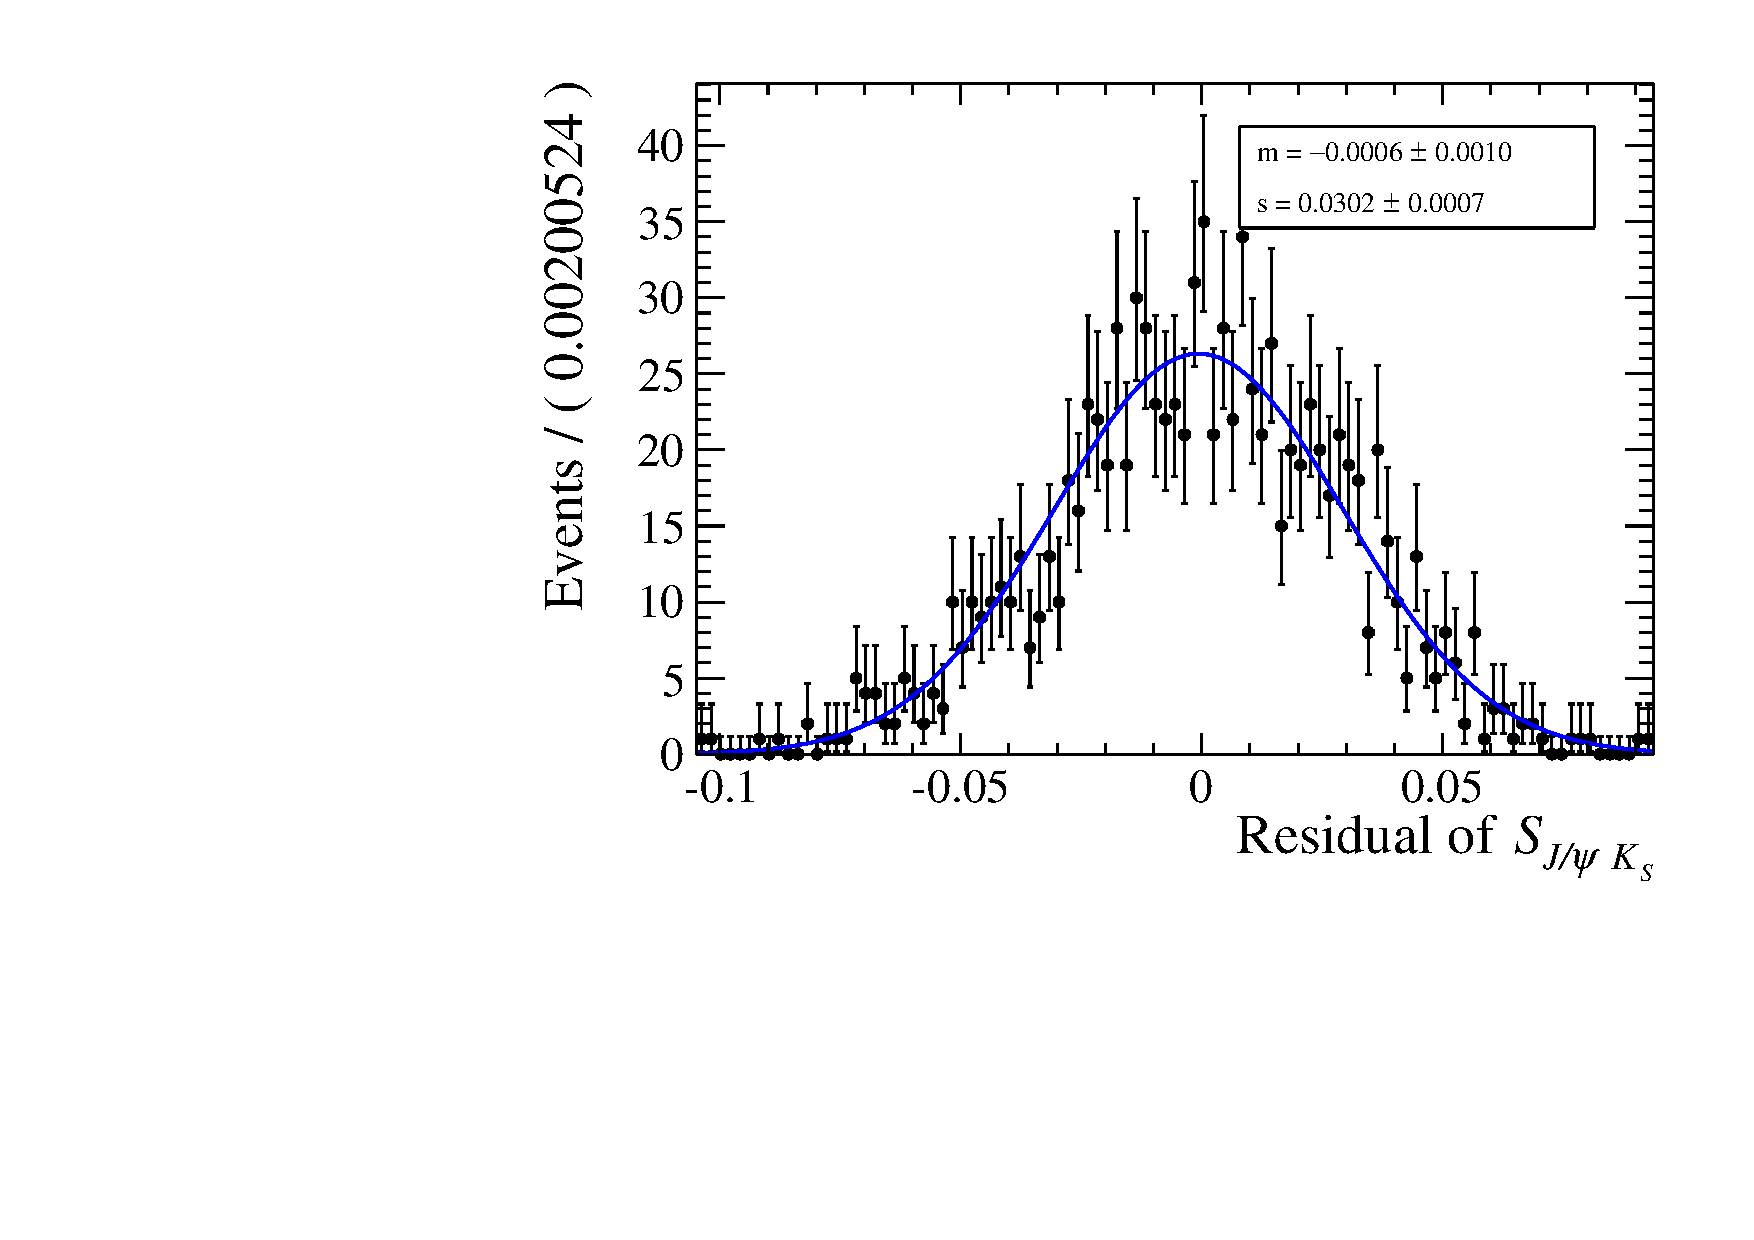
\includegraphics[width=0.49\textwidth]{private/content/appendices/figs/systematics_resolution_calibration_s_res.pdf}
  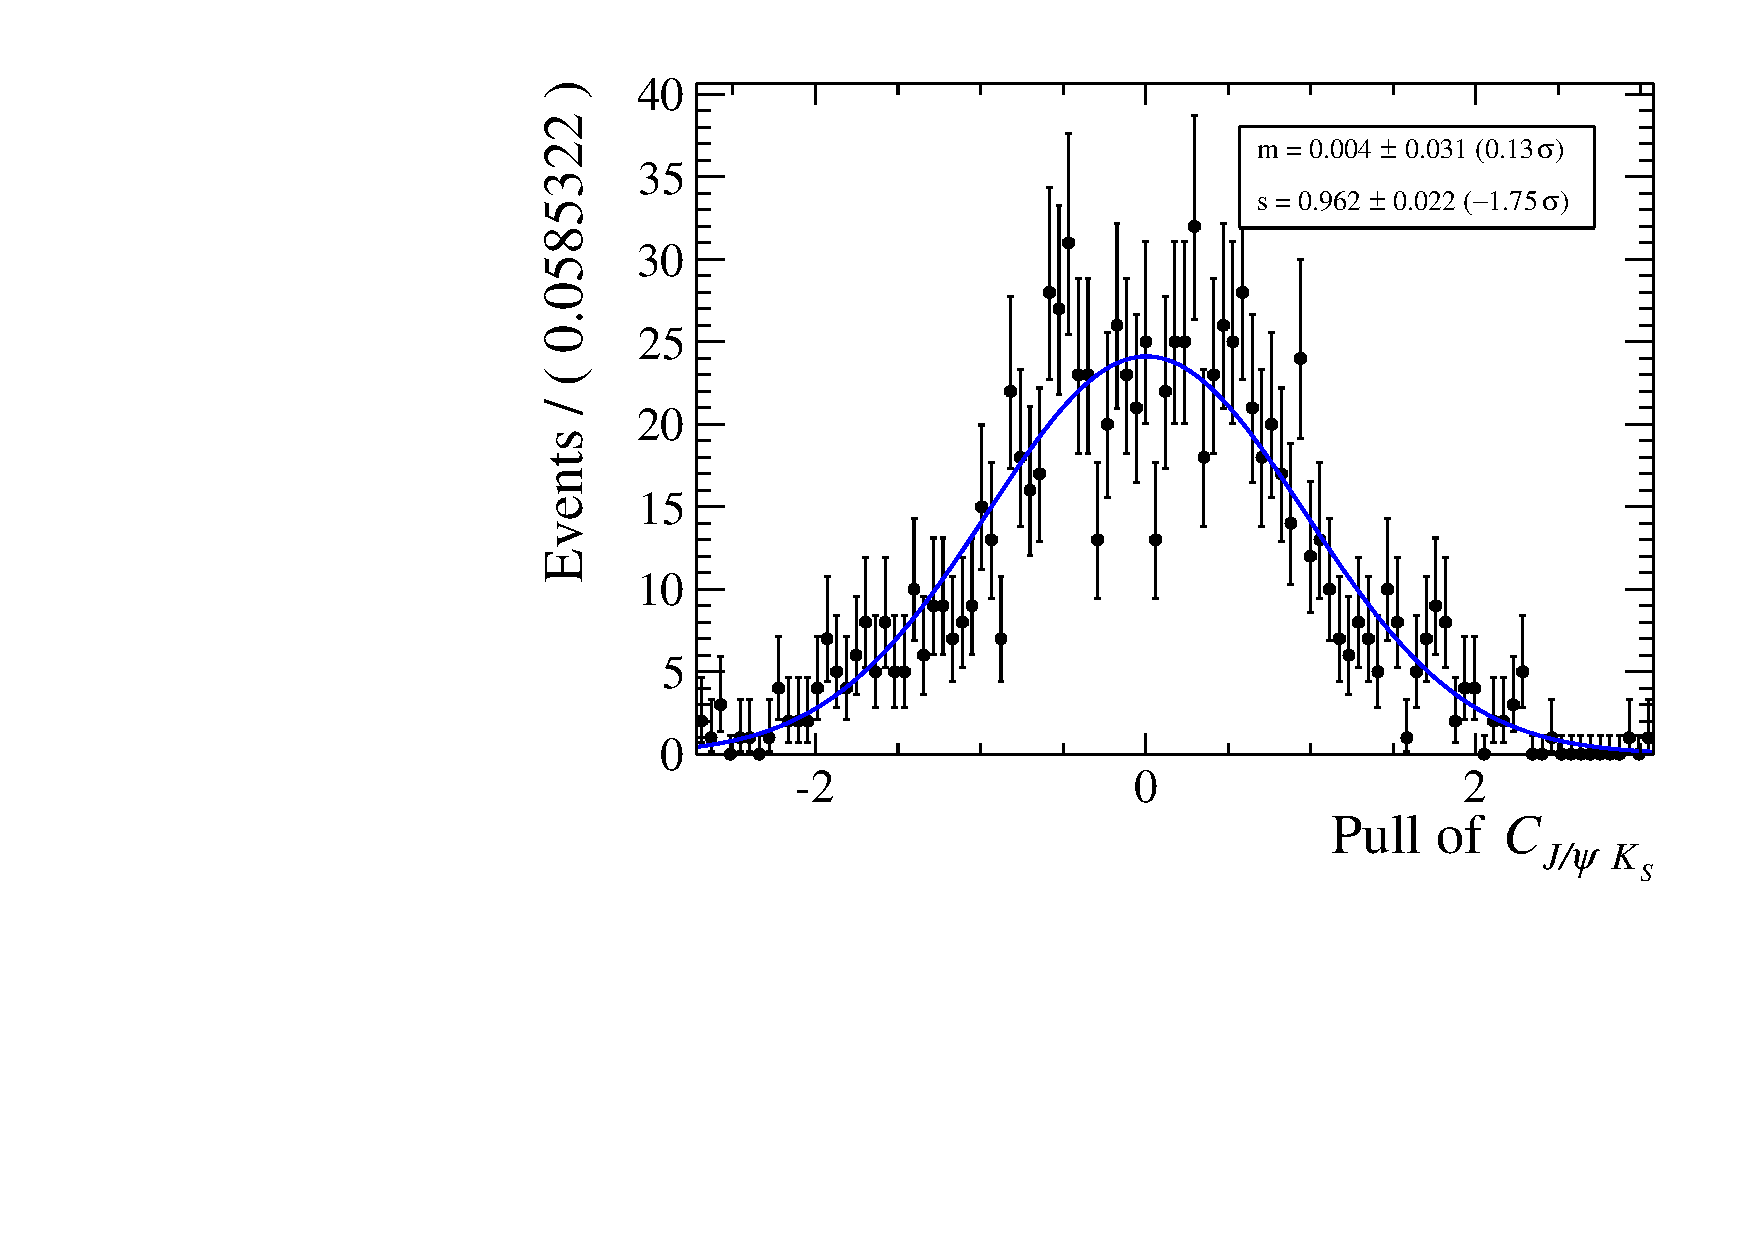
\includegraphics[width=0.49\textwidth]{private/content/appendices/figs/systematics_resolution_calibration_c_pull.pdf}\hfill
  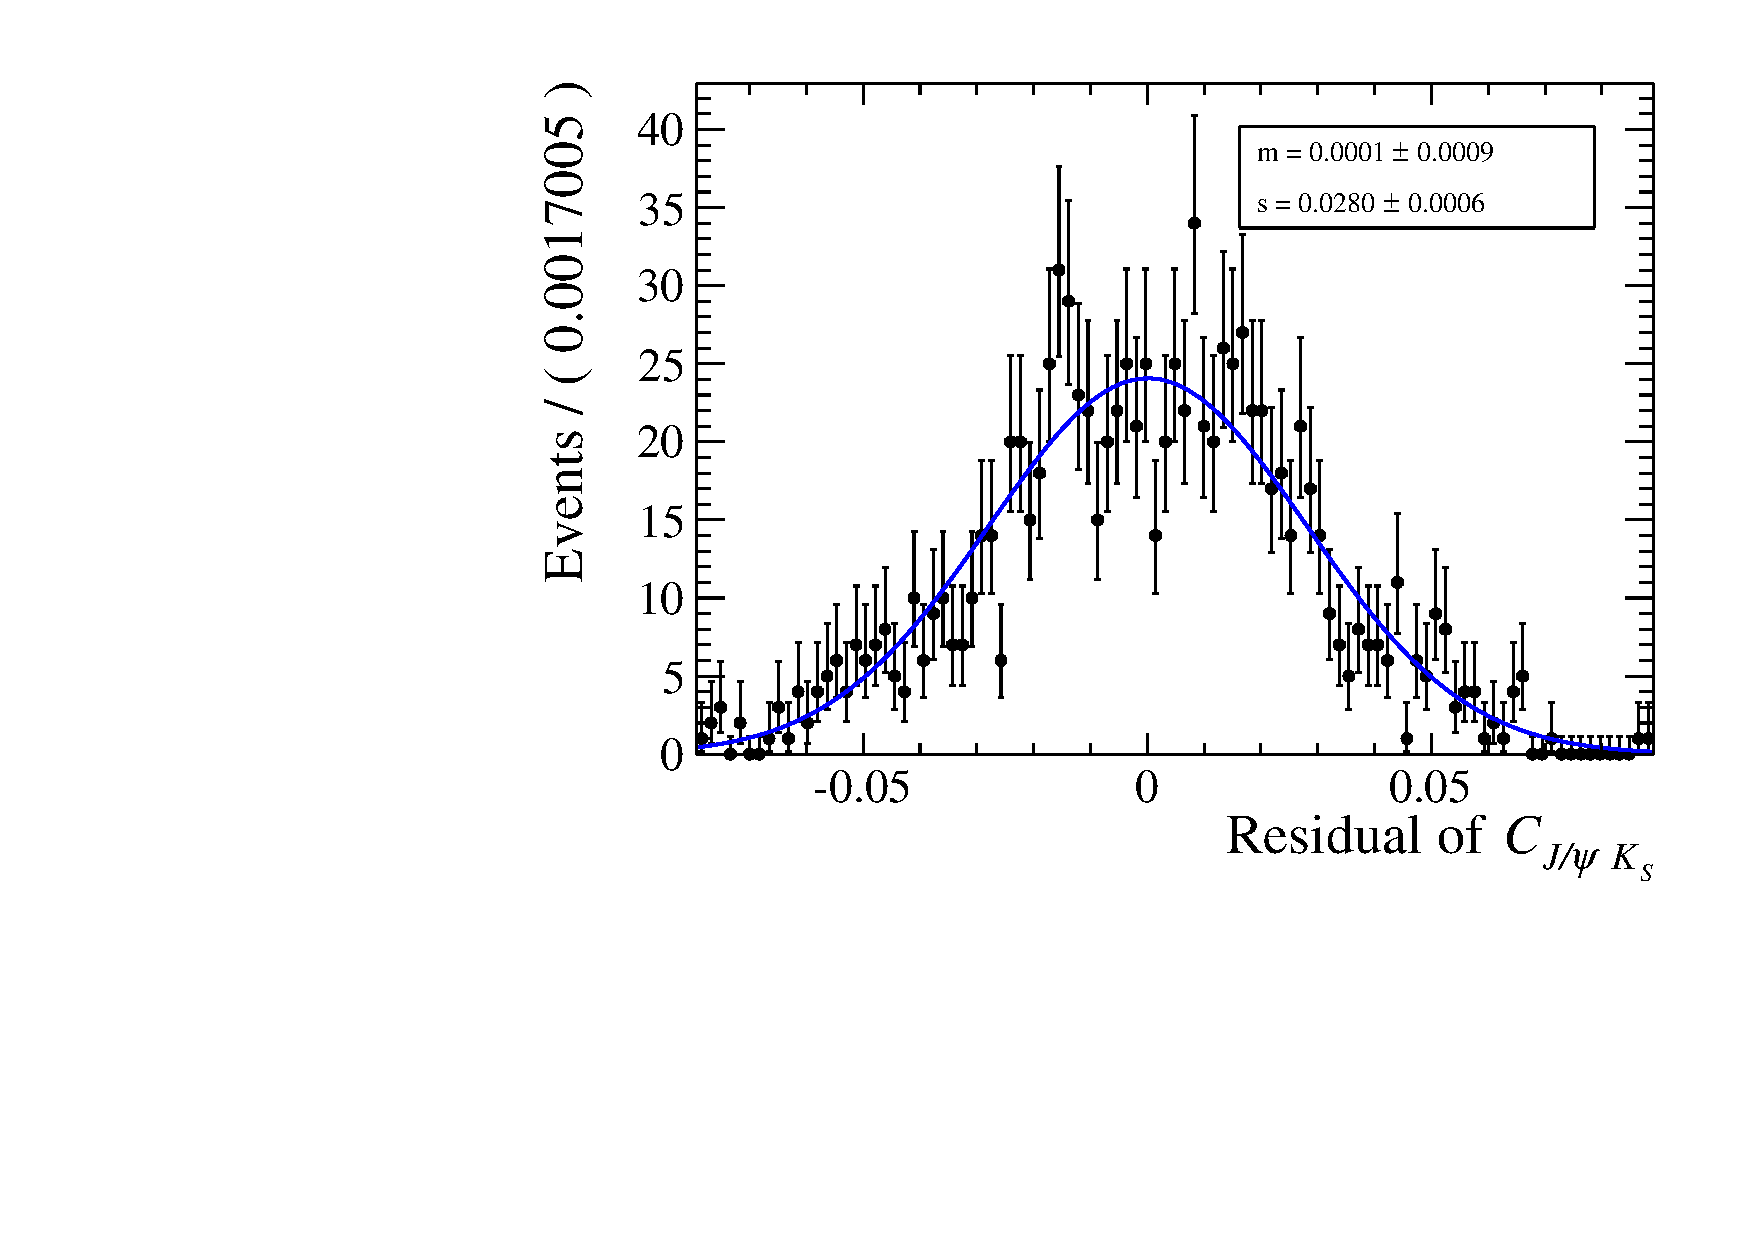
\includegraphics[width=0.49\textwidth]{private/content/appendices/figs/systematics_resolution_calibration_c_res.pdf}
\caption{Shown are (left) pull and (right) residual distributions of the
parameters (top) \SJpsiKS and (bottom) \CJpsiKS from a \ToyMC study of the
influence of the decay time resolution calibration model on the measurement of
the \CP parameters.}
\label{fig:app:measurement_of_sin2beta:systematics:systematics:resolution:calibration}
\end{figure}

\begin{figure}[h]
  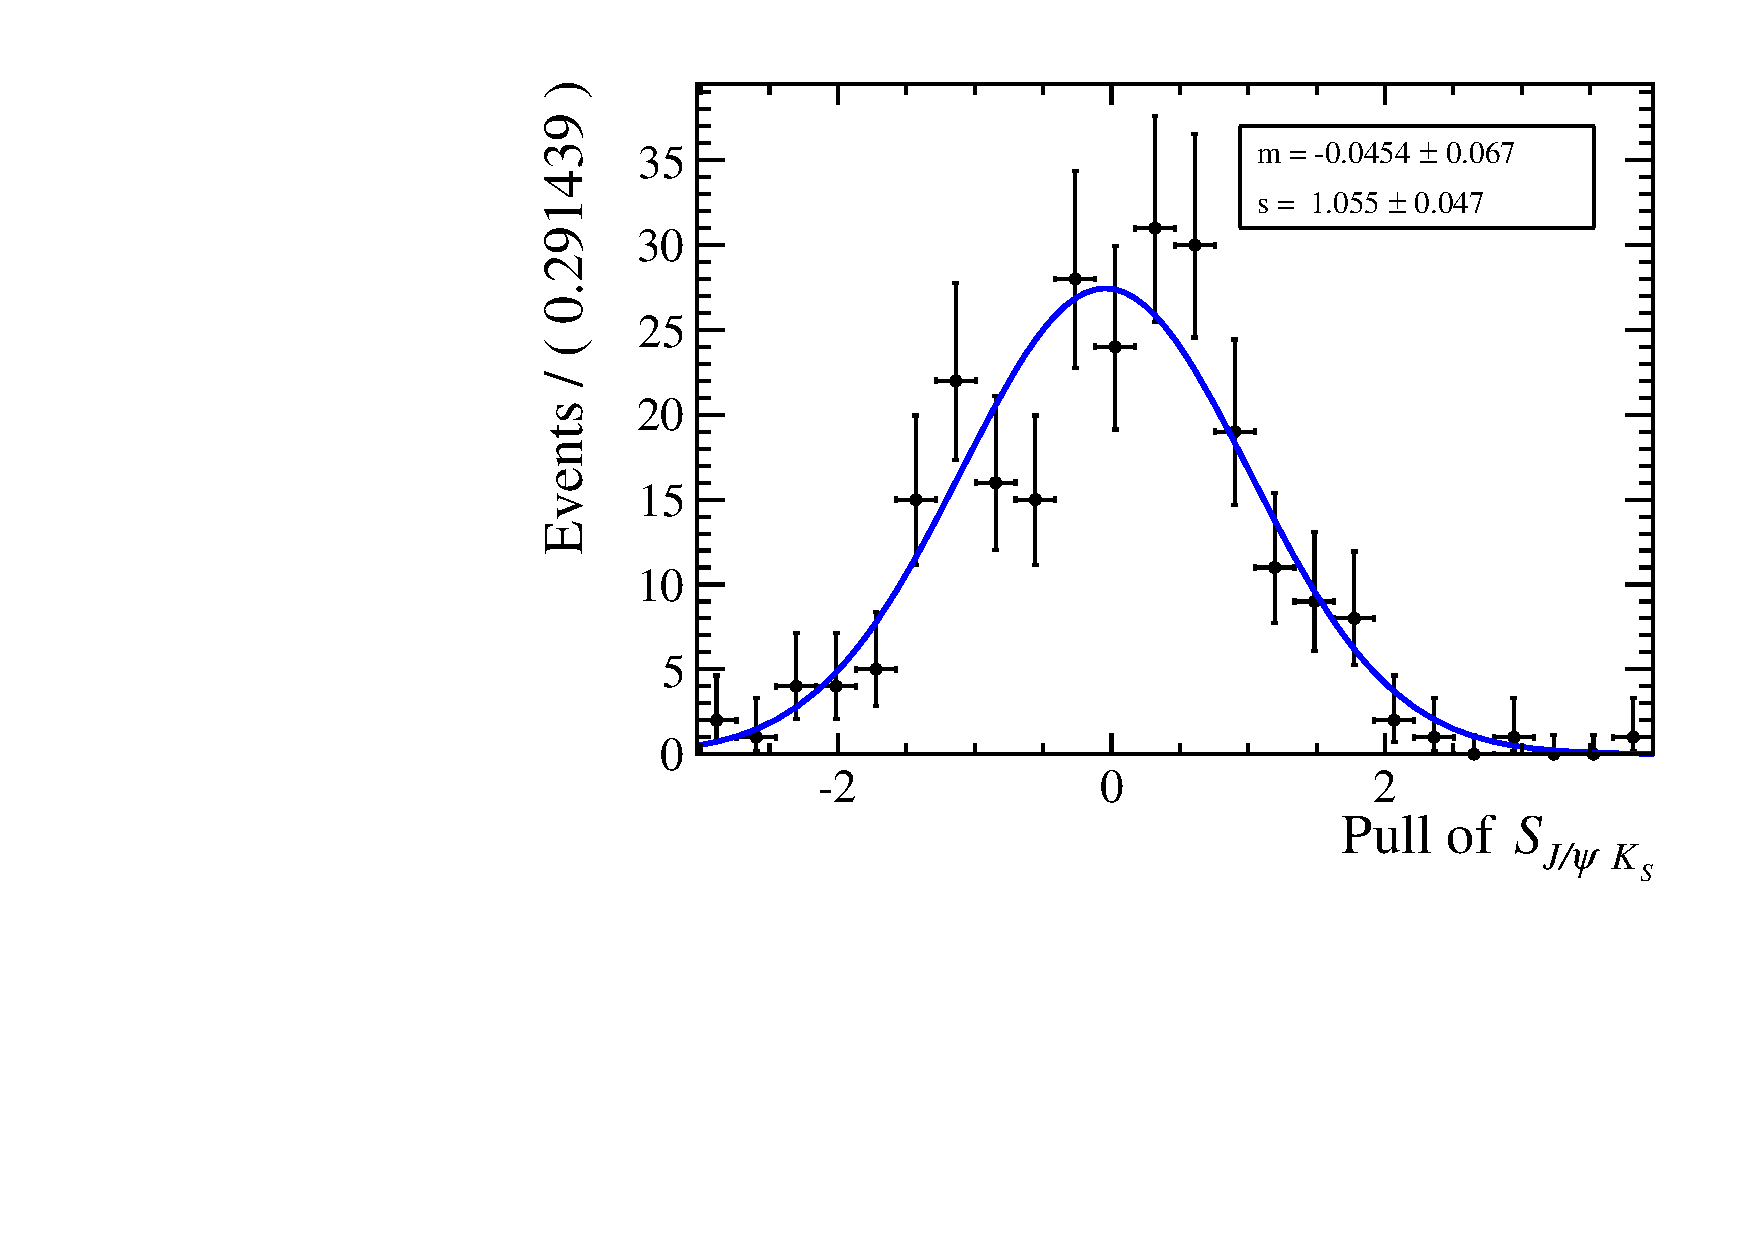
\includegraphics[width=0.49\textwidth]{private/content/appendices/figs/systematics_resolution_offset_s_pull.pdf}\hfill
  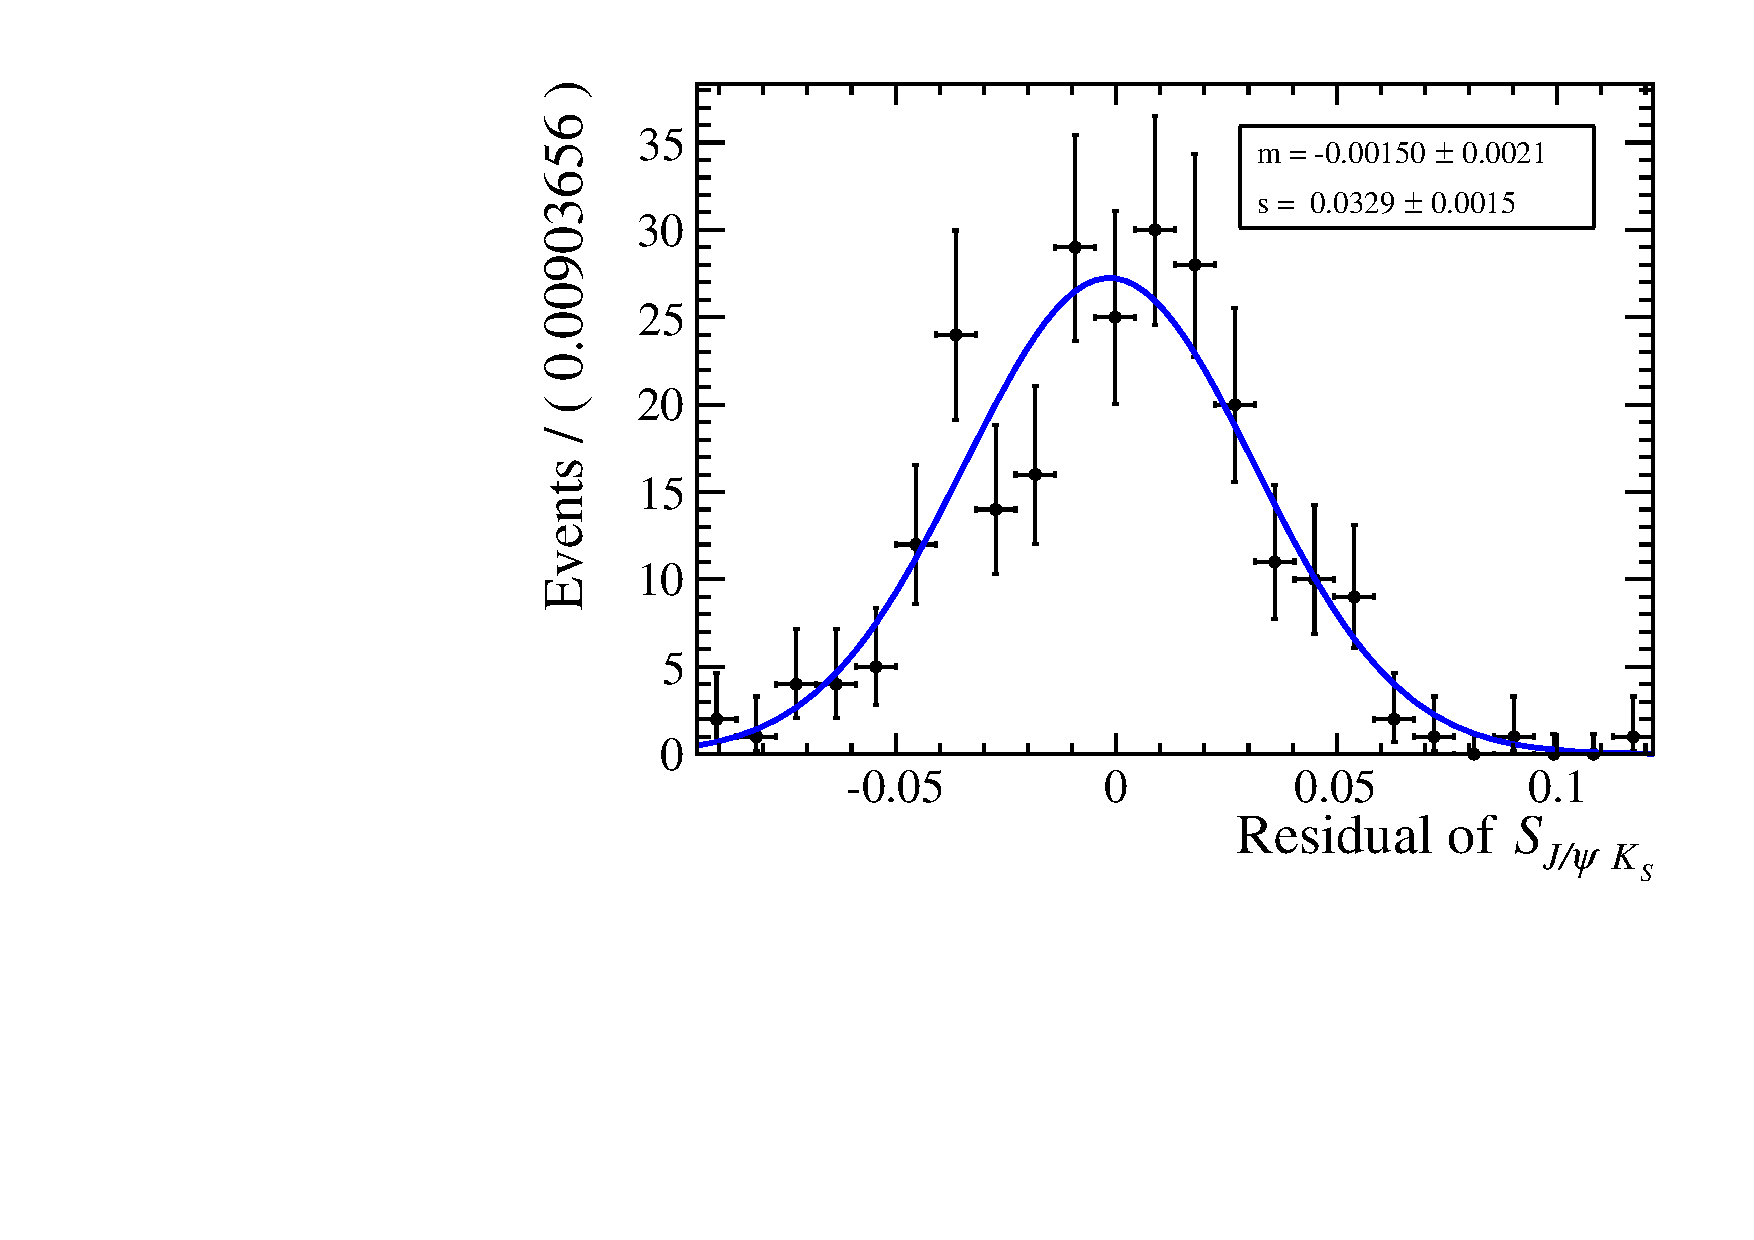
\includegraphics[width=0.49\textwidth]{private/content/appendices/figs/systematics_resolution_offset_s_res.pdf}
  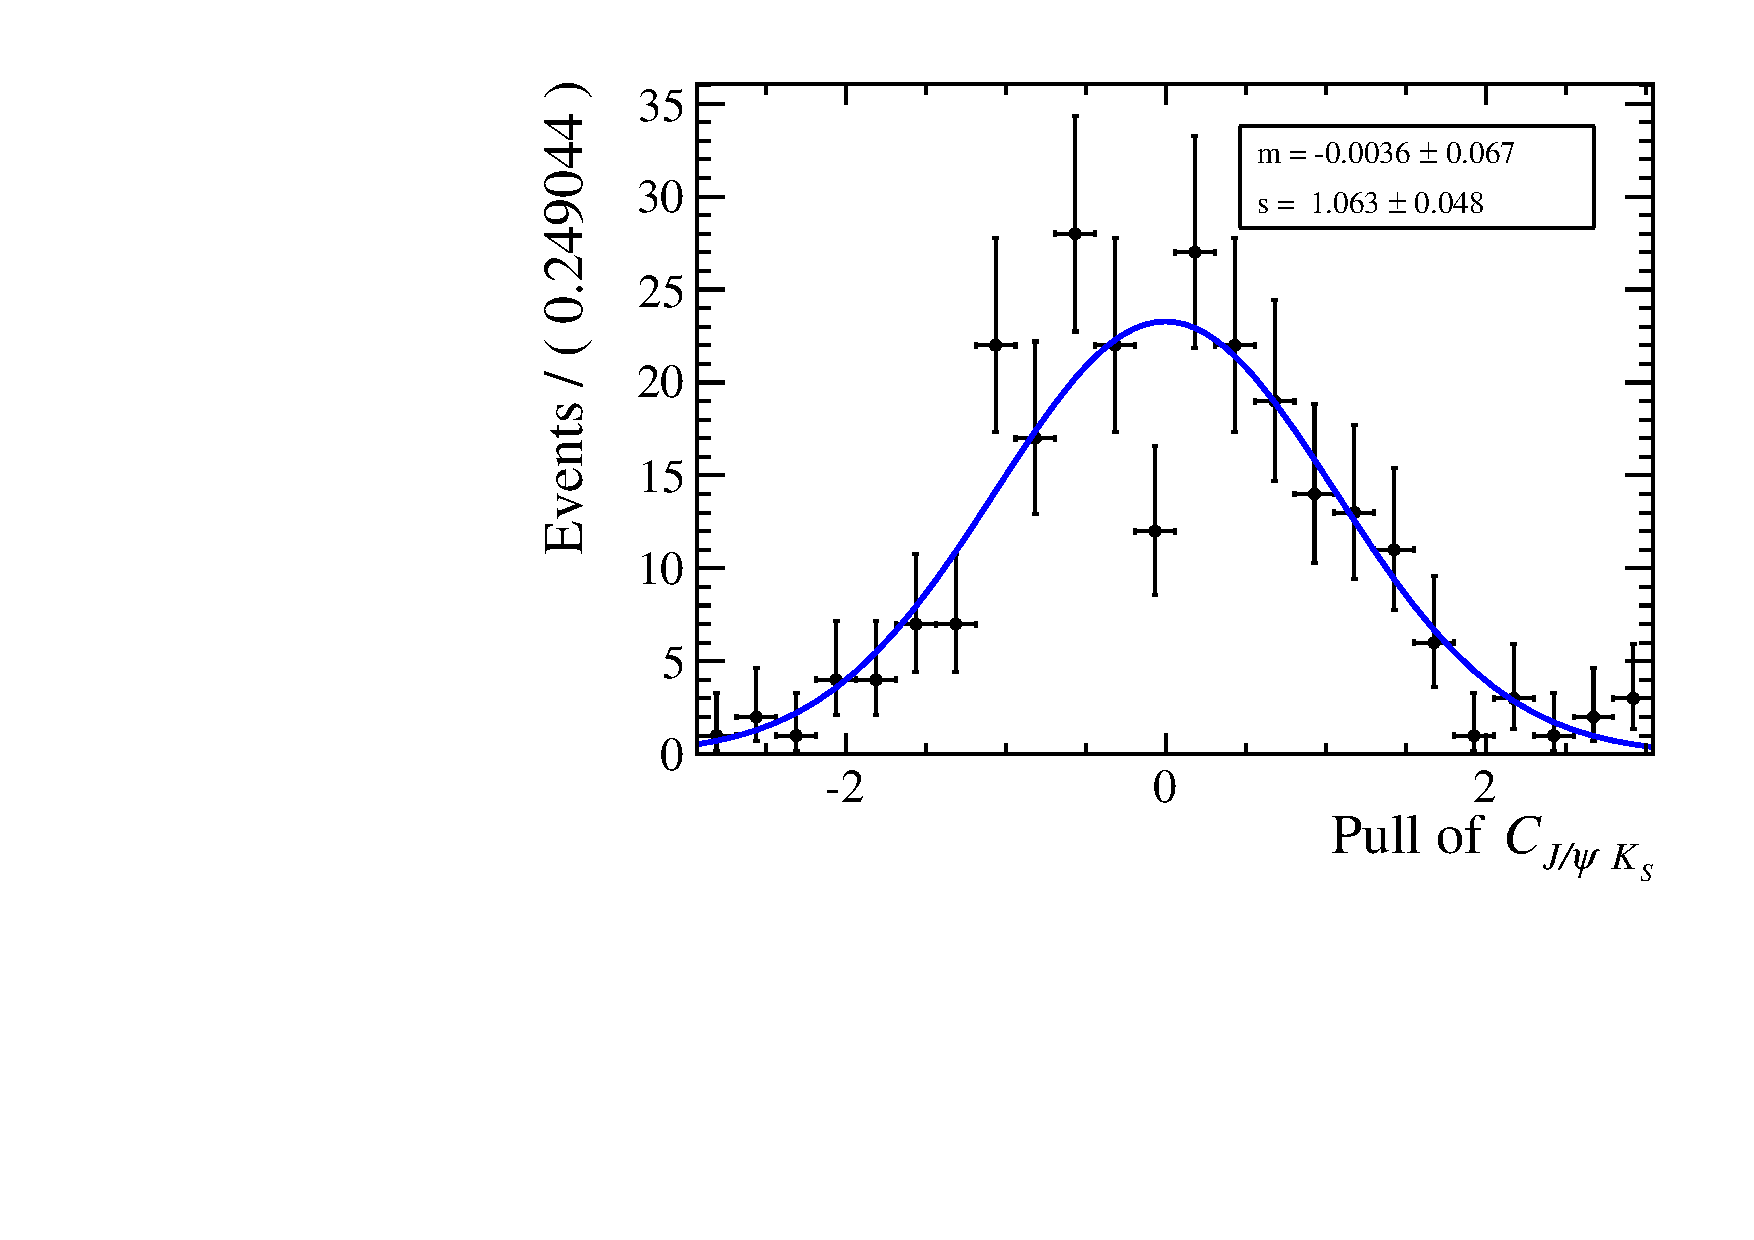
\includegraphics[width=0.49\textwidth]{private/content/appendices/figs/systematics_resolution_offset_c_pull.pdf}\hfill
  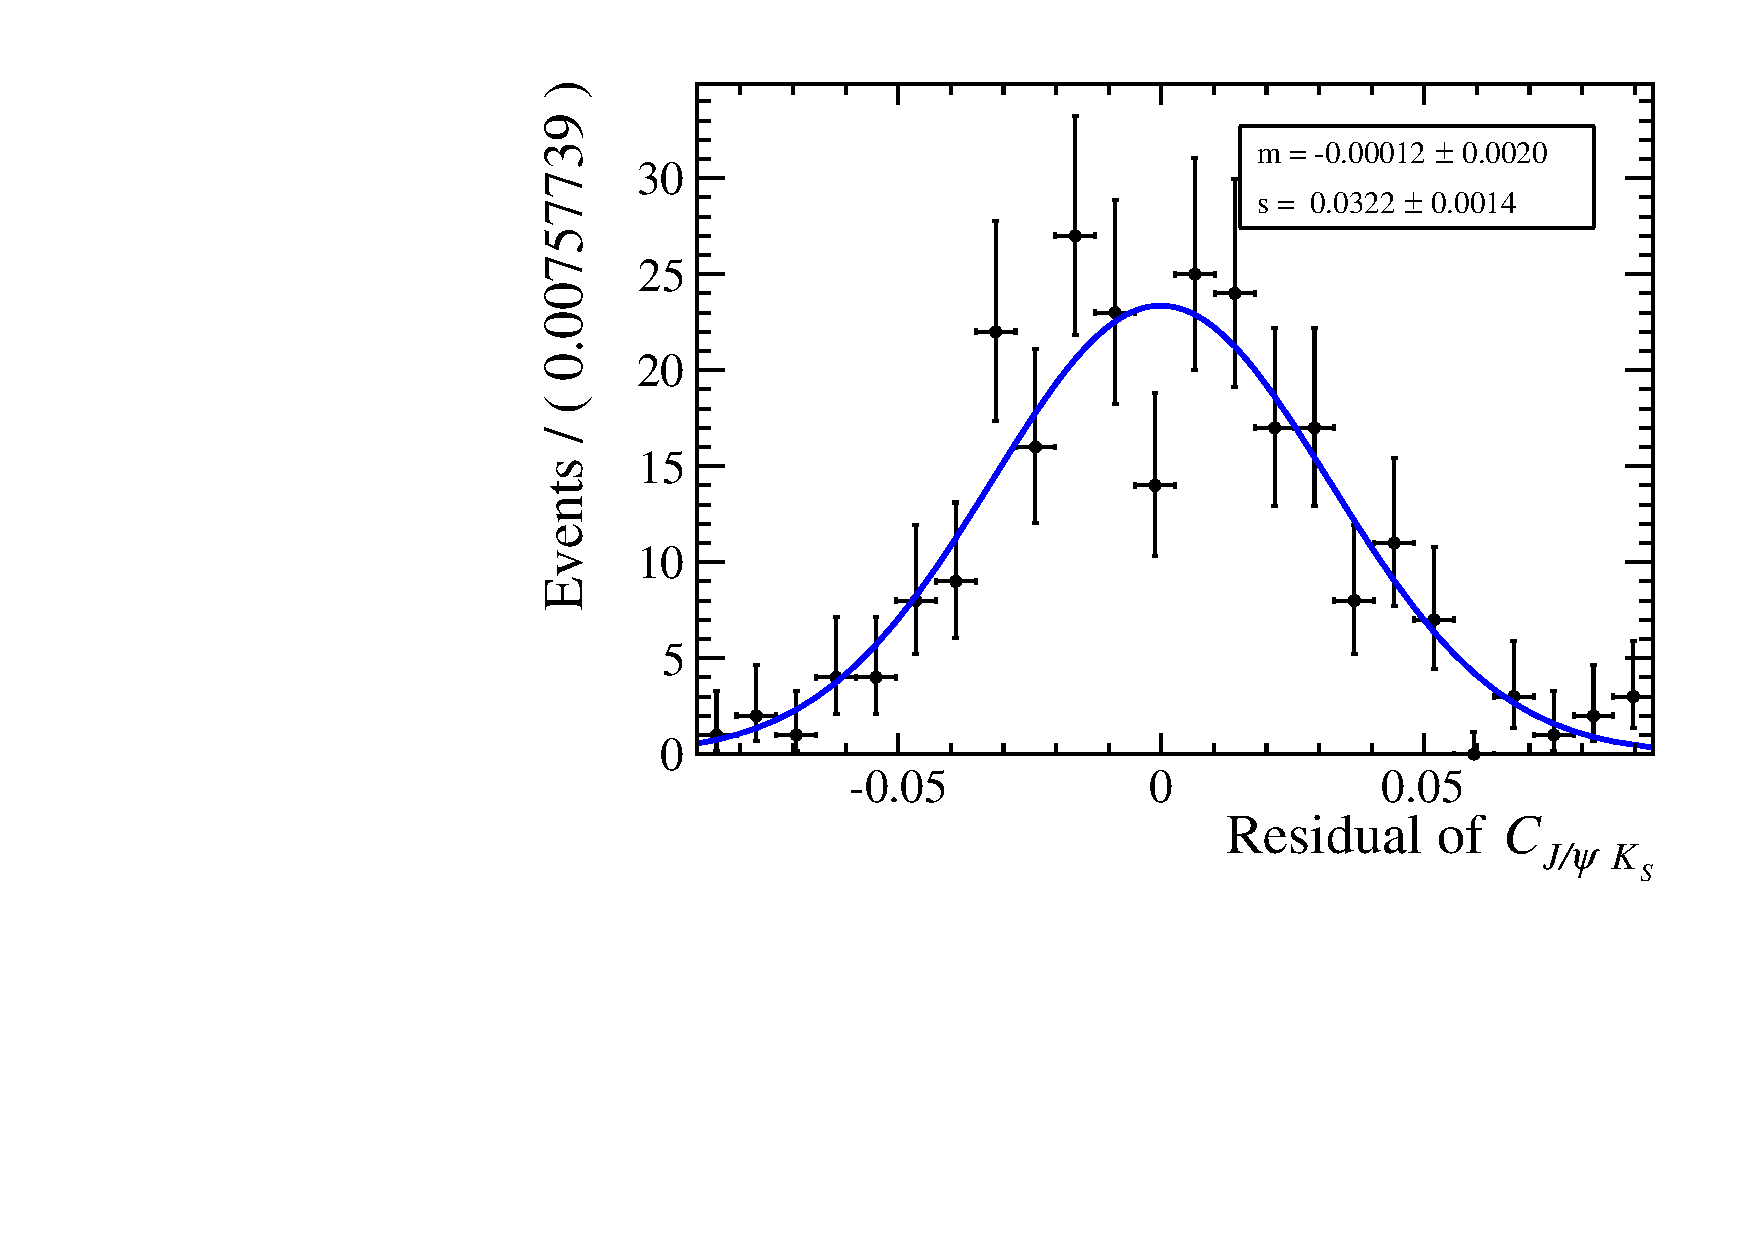
\includegraphics[width=0.49\textwidth]{private/content/appendices/figs/systematics_resolution_offset_c_res.pdf}
\caption{Shown are (left) pull and (right) residual distributions of the
parameters (top) \SJpsiKS and (bottom) \CJpsiKS from a \ToyMC study of the
influence of neglecting a non-zero offset in the decay time resolution
calibration model on the measurement of the \CP parameters.}
\label{fig:app:measurement_of_sin2beta:systematics:systematics:resolution:offset}
\end{figure}

\begin{figure}[h]
  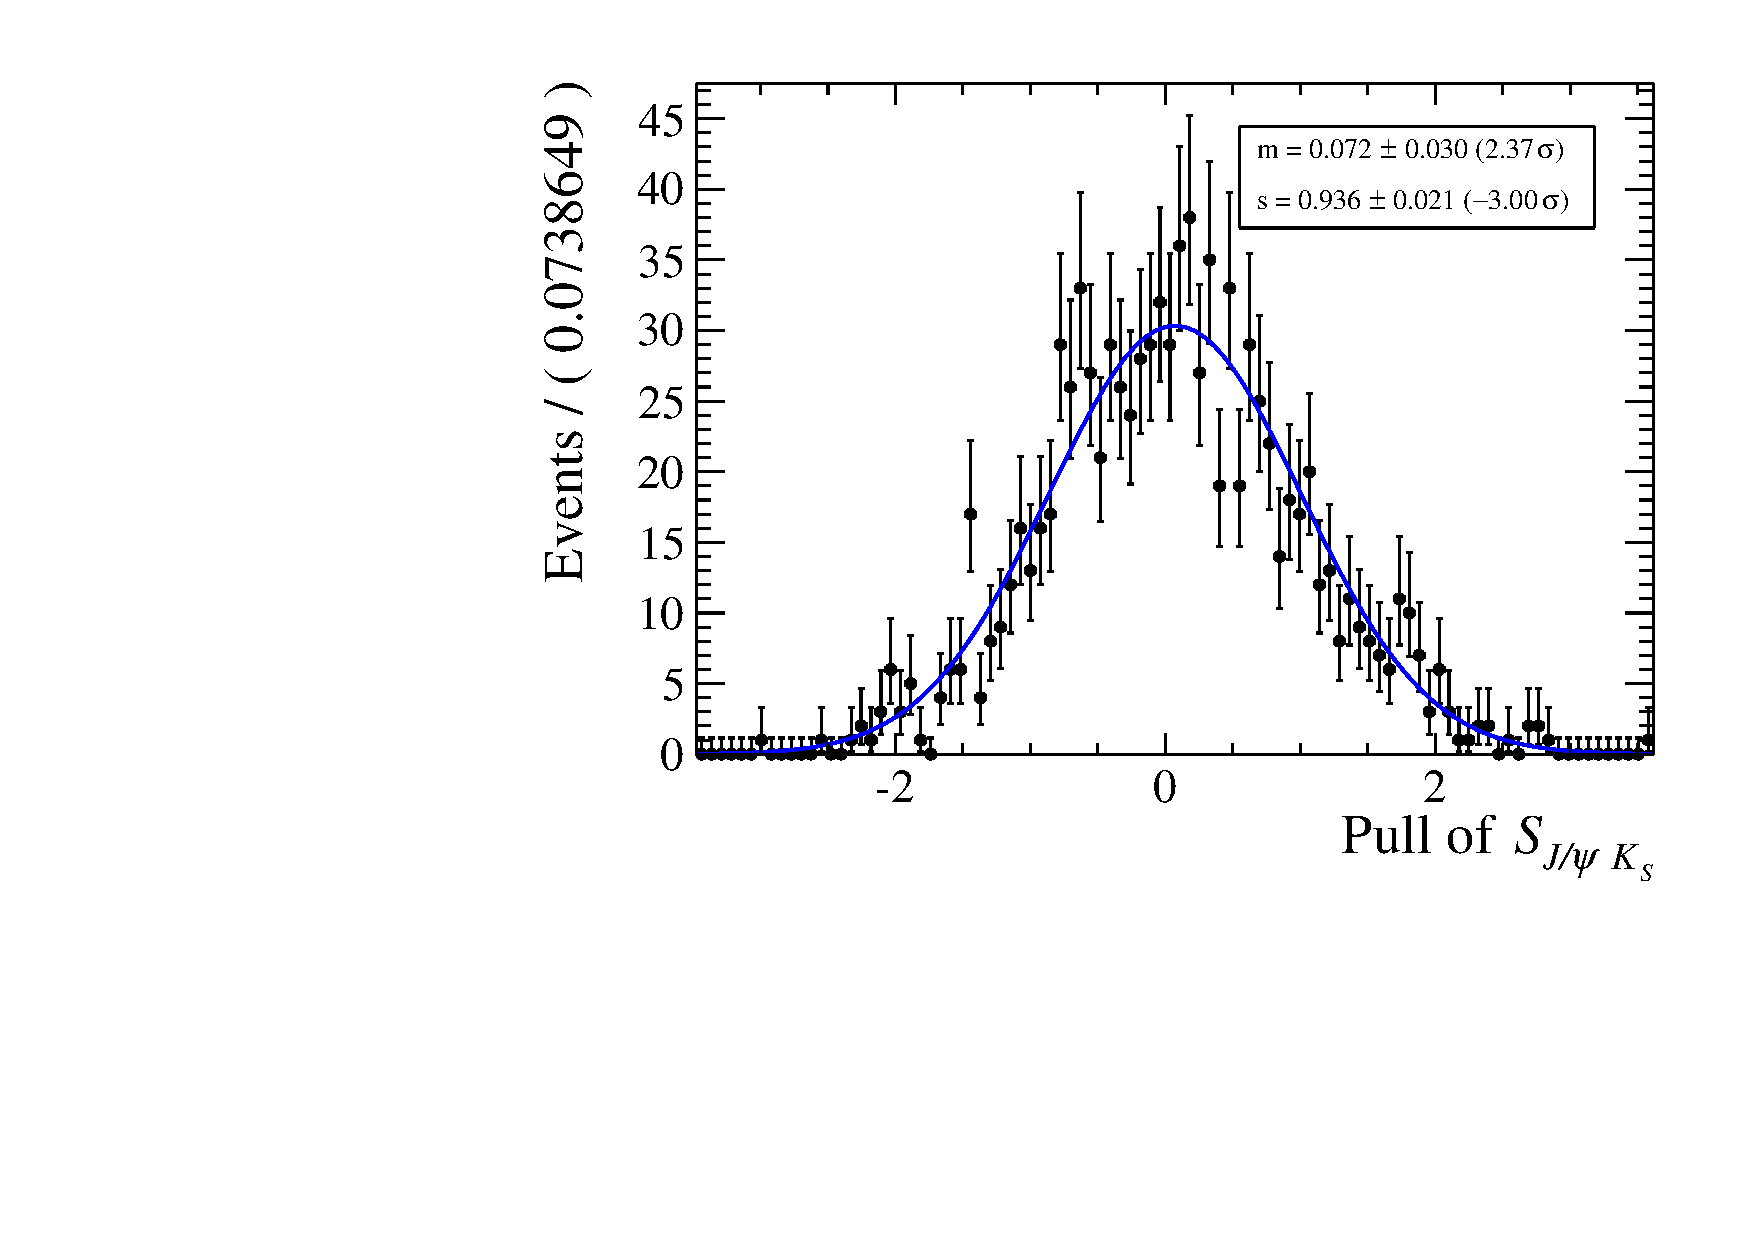
\includegraphics[width=0.49\textwidth]{private/content/appendices/figs/systematics_resolution_wrongpv_s_pull.pdf}\hfill
  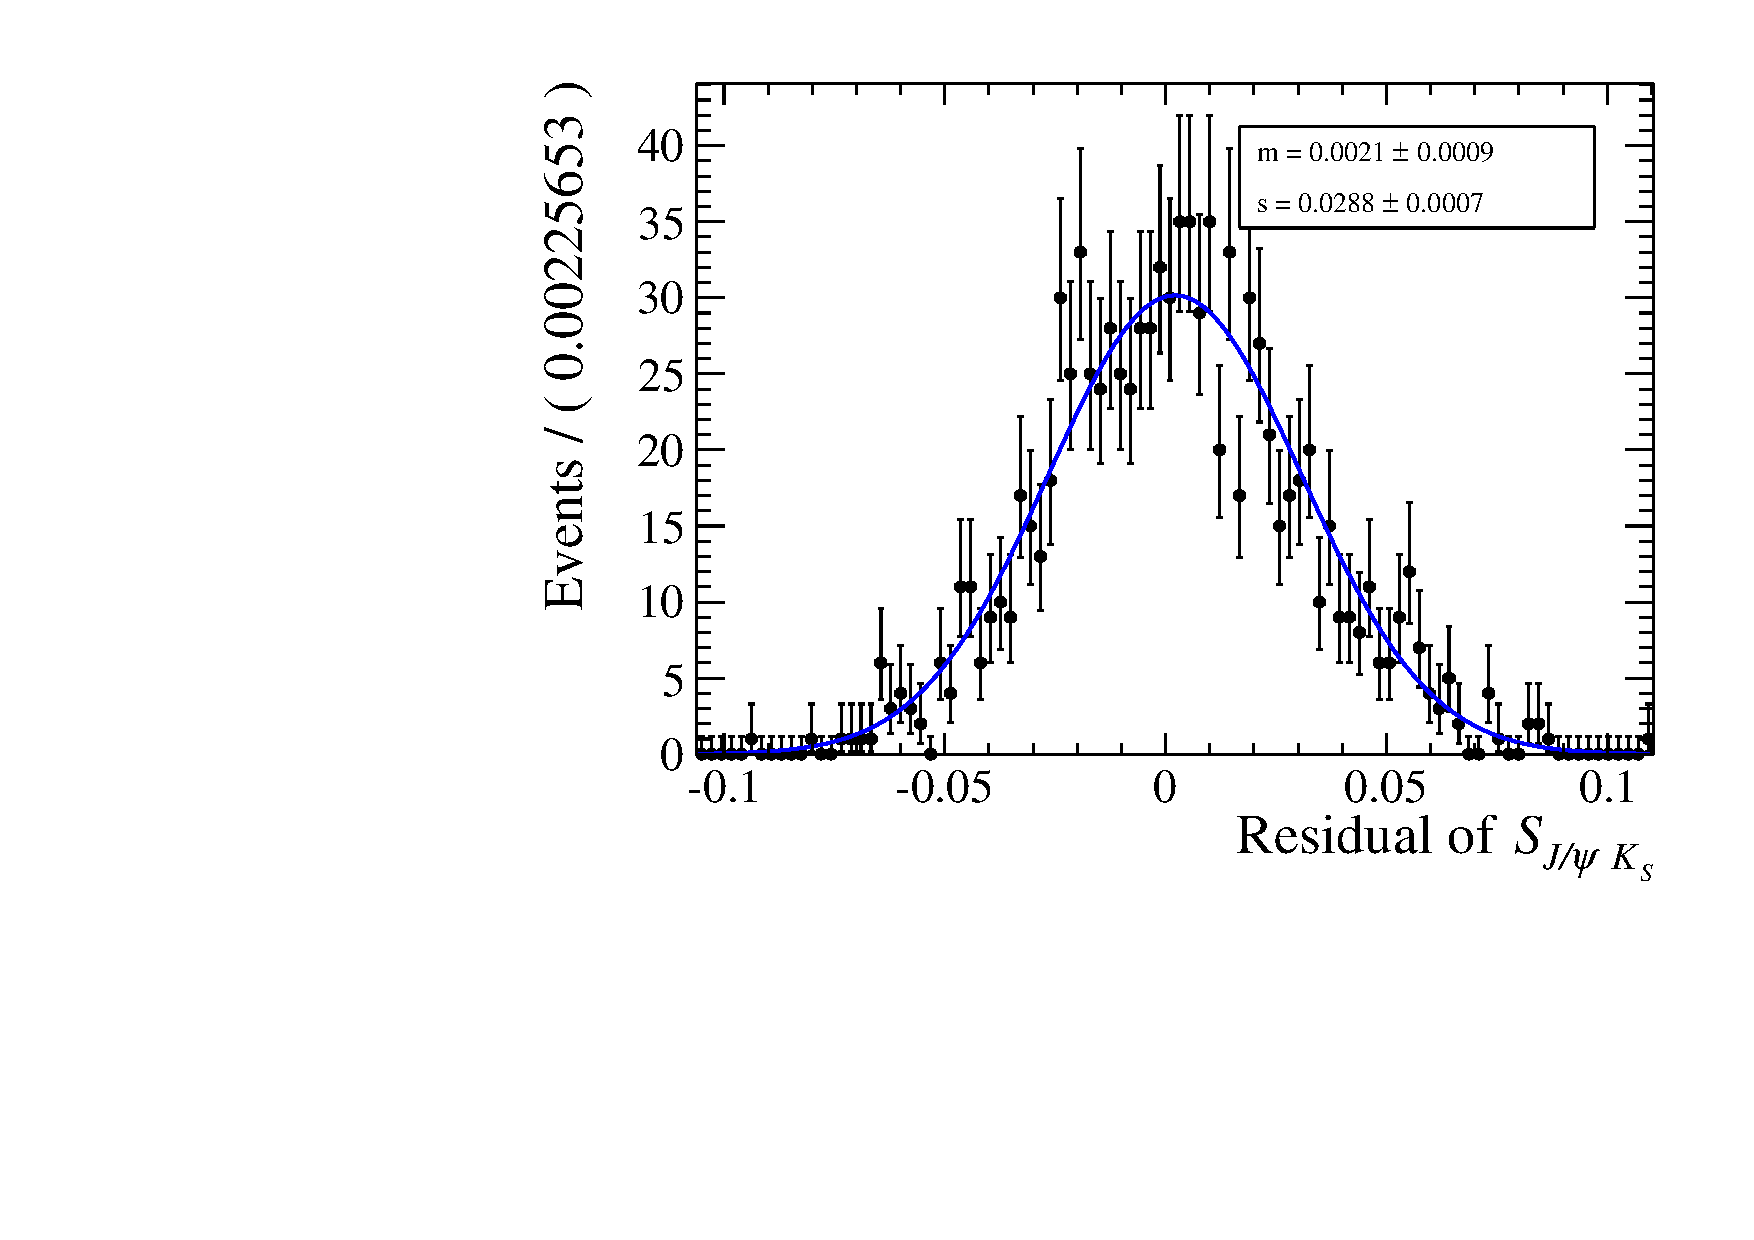
\includegraphics[width=0.49\textwidth]{private/content/appendices/figs/systematics_resolution_wrongpv_s_res.pdf}
  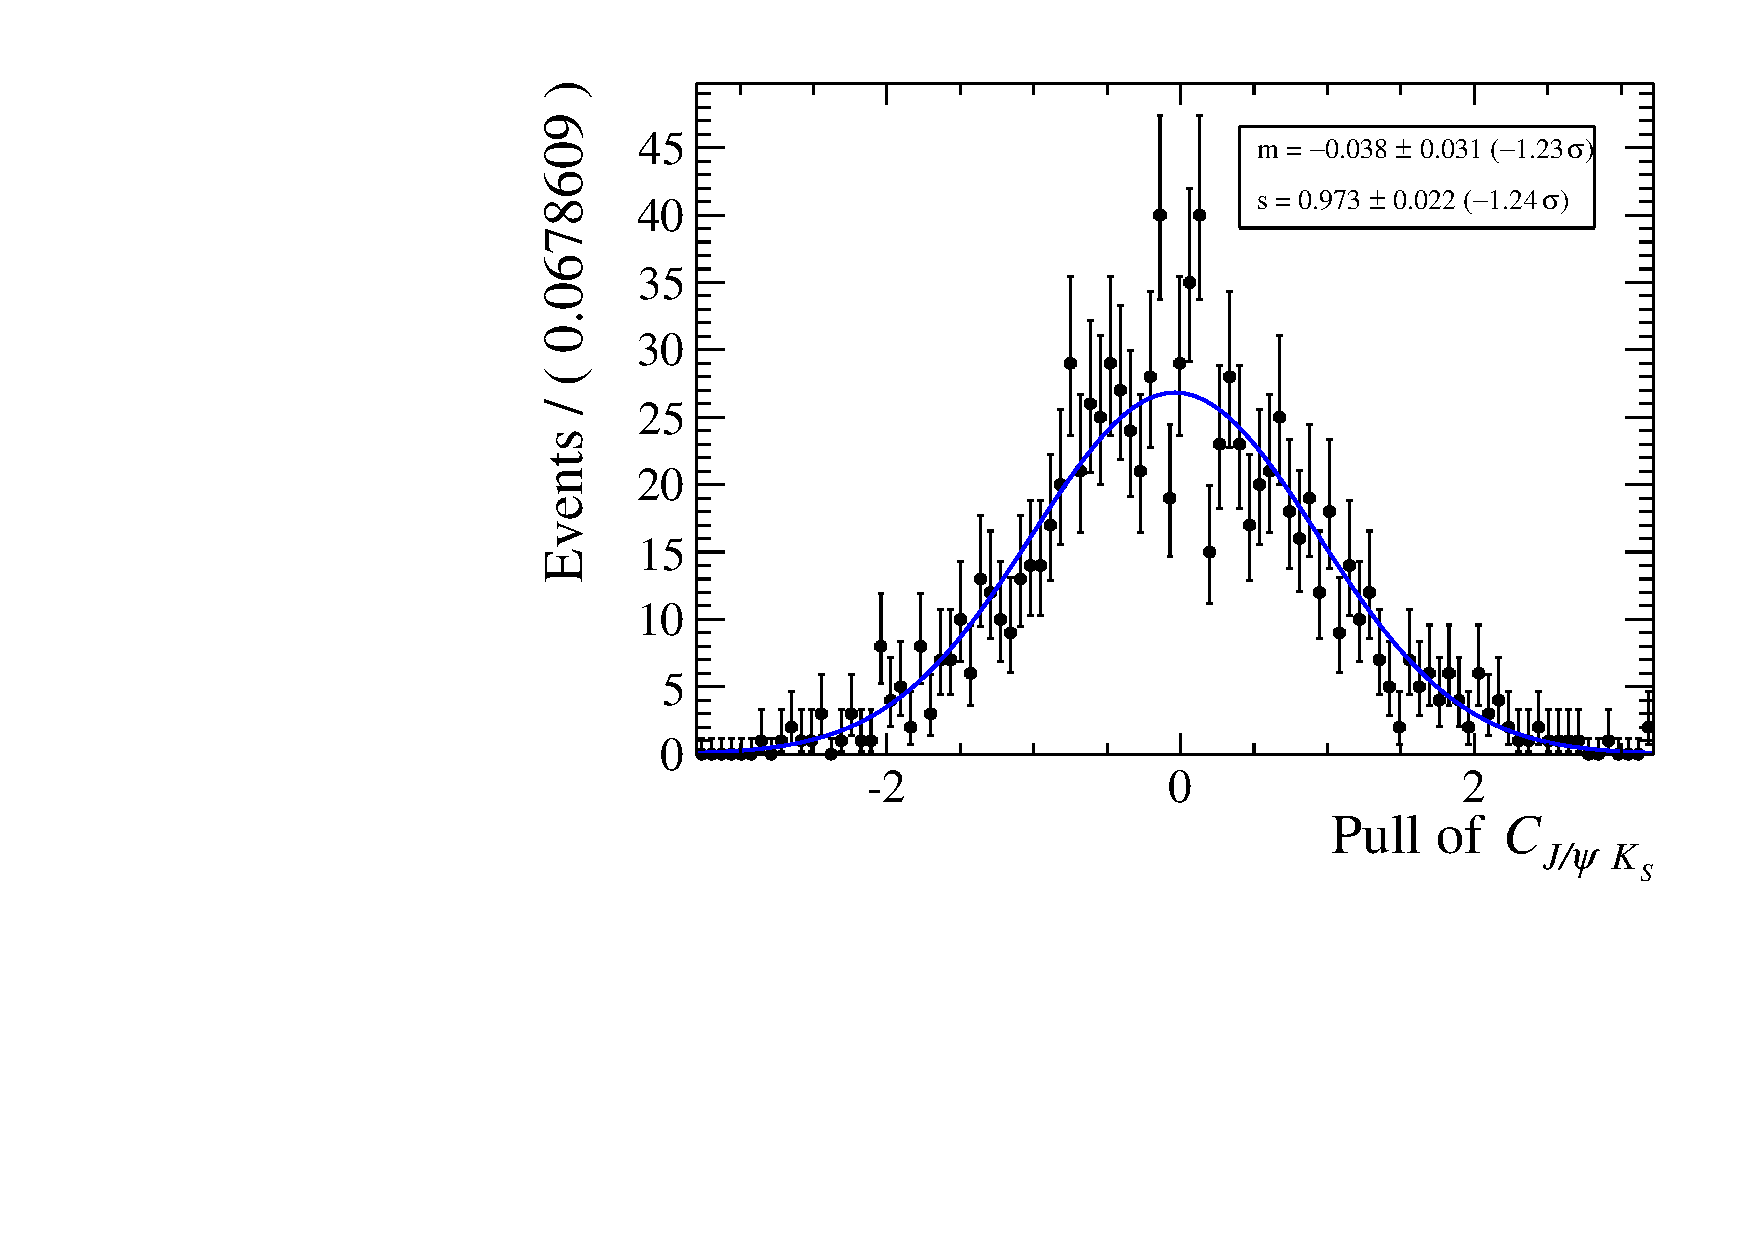
\includegraphics[width=0.49\textwidth]{private/content/appendices/figs/systematics_resolution_wrongpv_c_pull.pdf}\hfill
  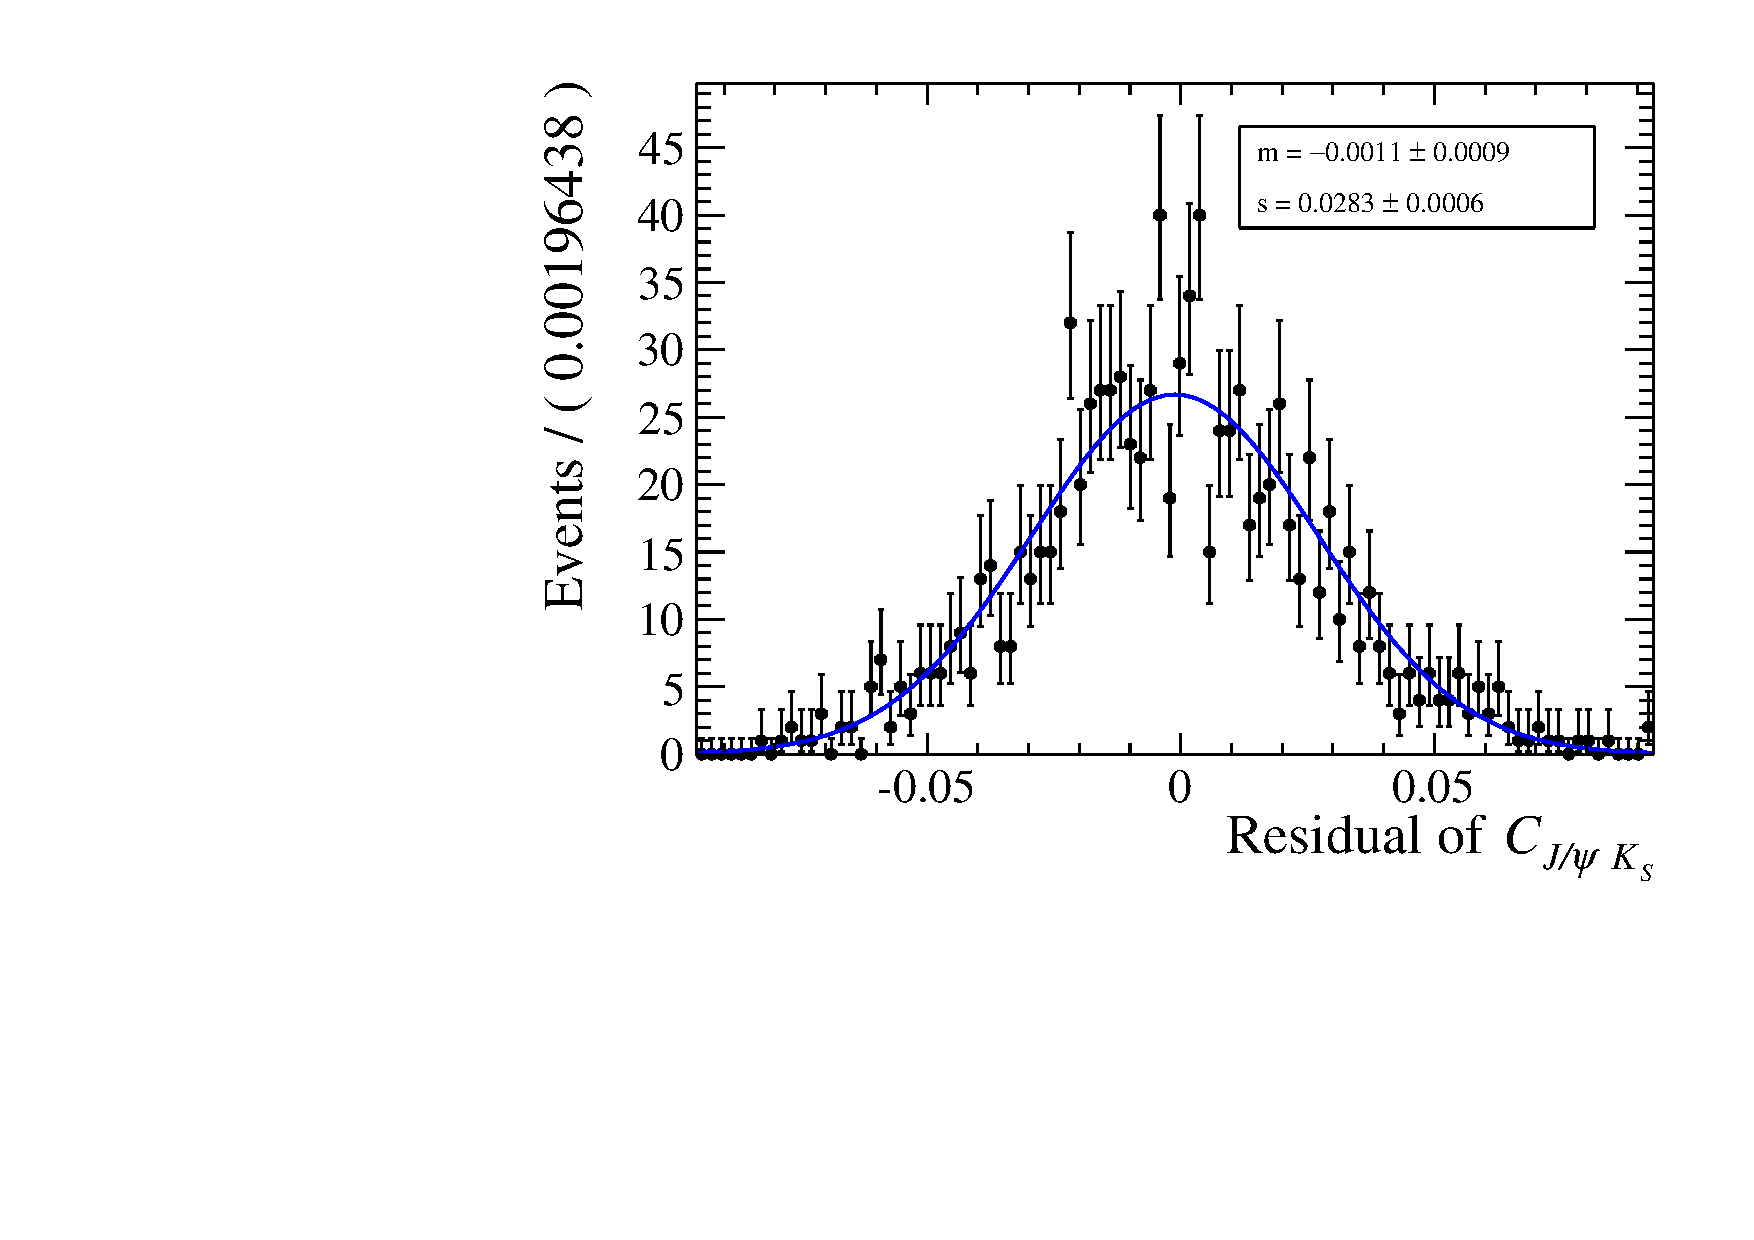
\includegraphics[width=0.49\textwidth]{private/content/appendices/figs/systematics_resolution_wrongpv_c_res.pdf}
\caption{Shown are (left) pull and (right) residual distributions of the
parameters (top) \SJpsiKS and (bottom) \CJpsiKS from a \ToyMC study of the
influence of the fraction of candidates with a wrong \PV association on the
measurement of the \CP parameters.}
\label{fig:app:measurement_of_sin2beta:systematics:systematics:resolution:wrong_pv}
\end{figure}

\clearpage
% ..............................................................................
\subsubsection{Decay time acceptance}
\label{sec:app:measurement_of_sin2beta:systematics:systematics:acceptance}

\begin{figure}[h]
  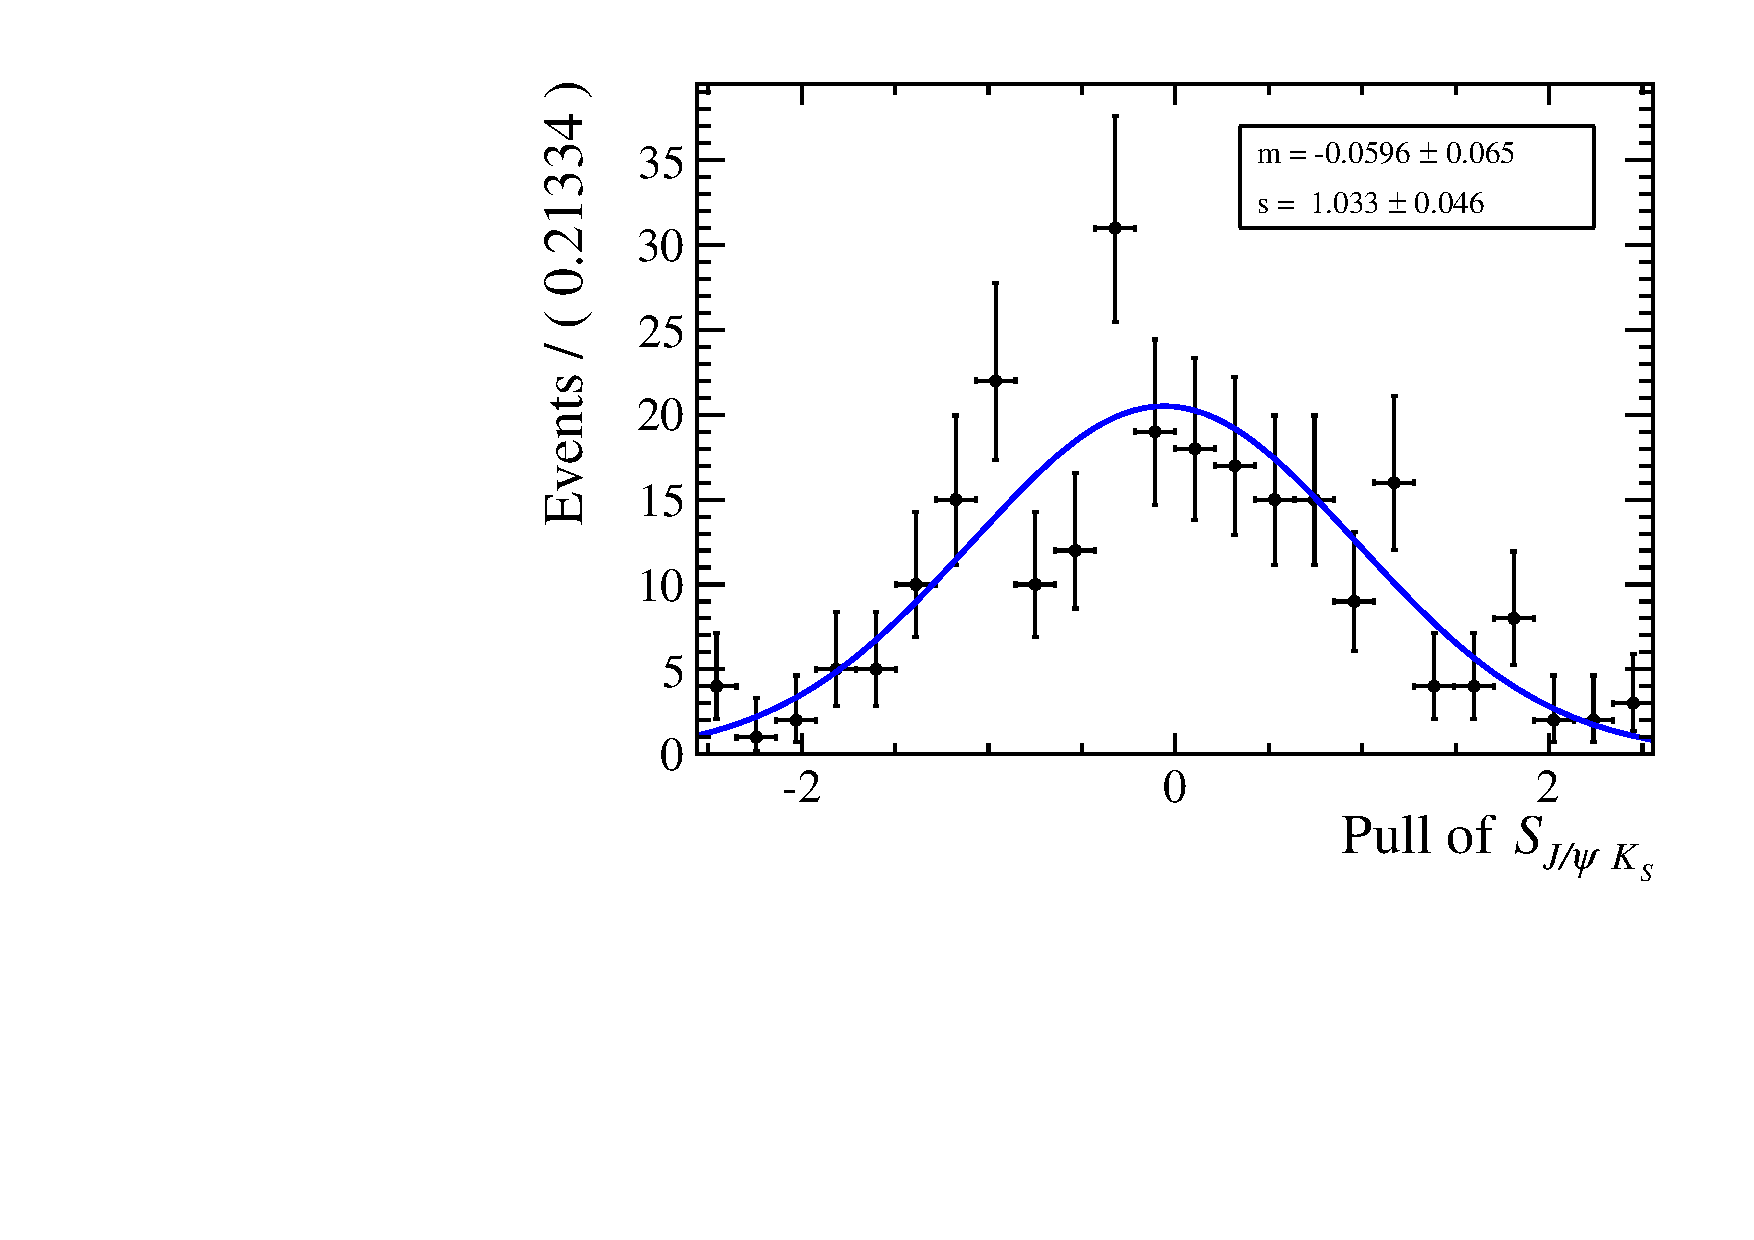
\includegraphics[width=0.49\textwidth]{private/content/appendices/figs/systematics_acc_lower_s_pull.pdf}\hfill
  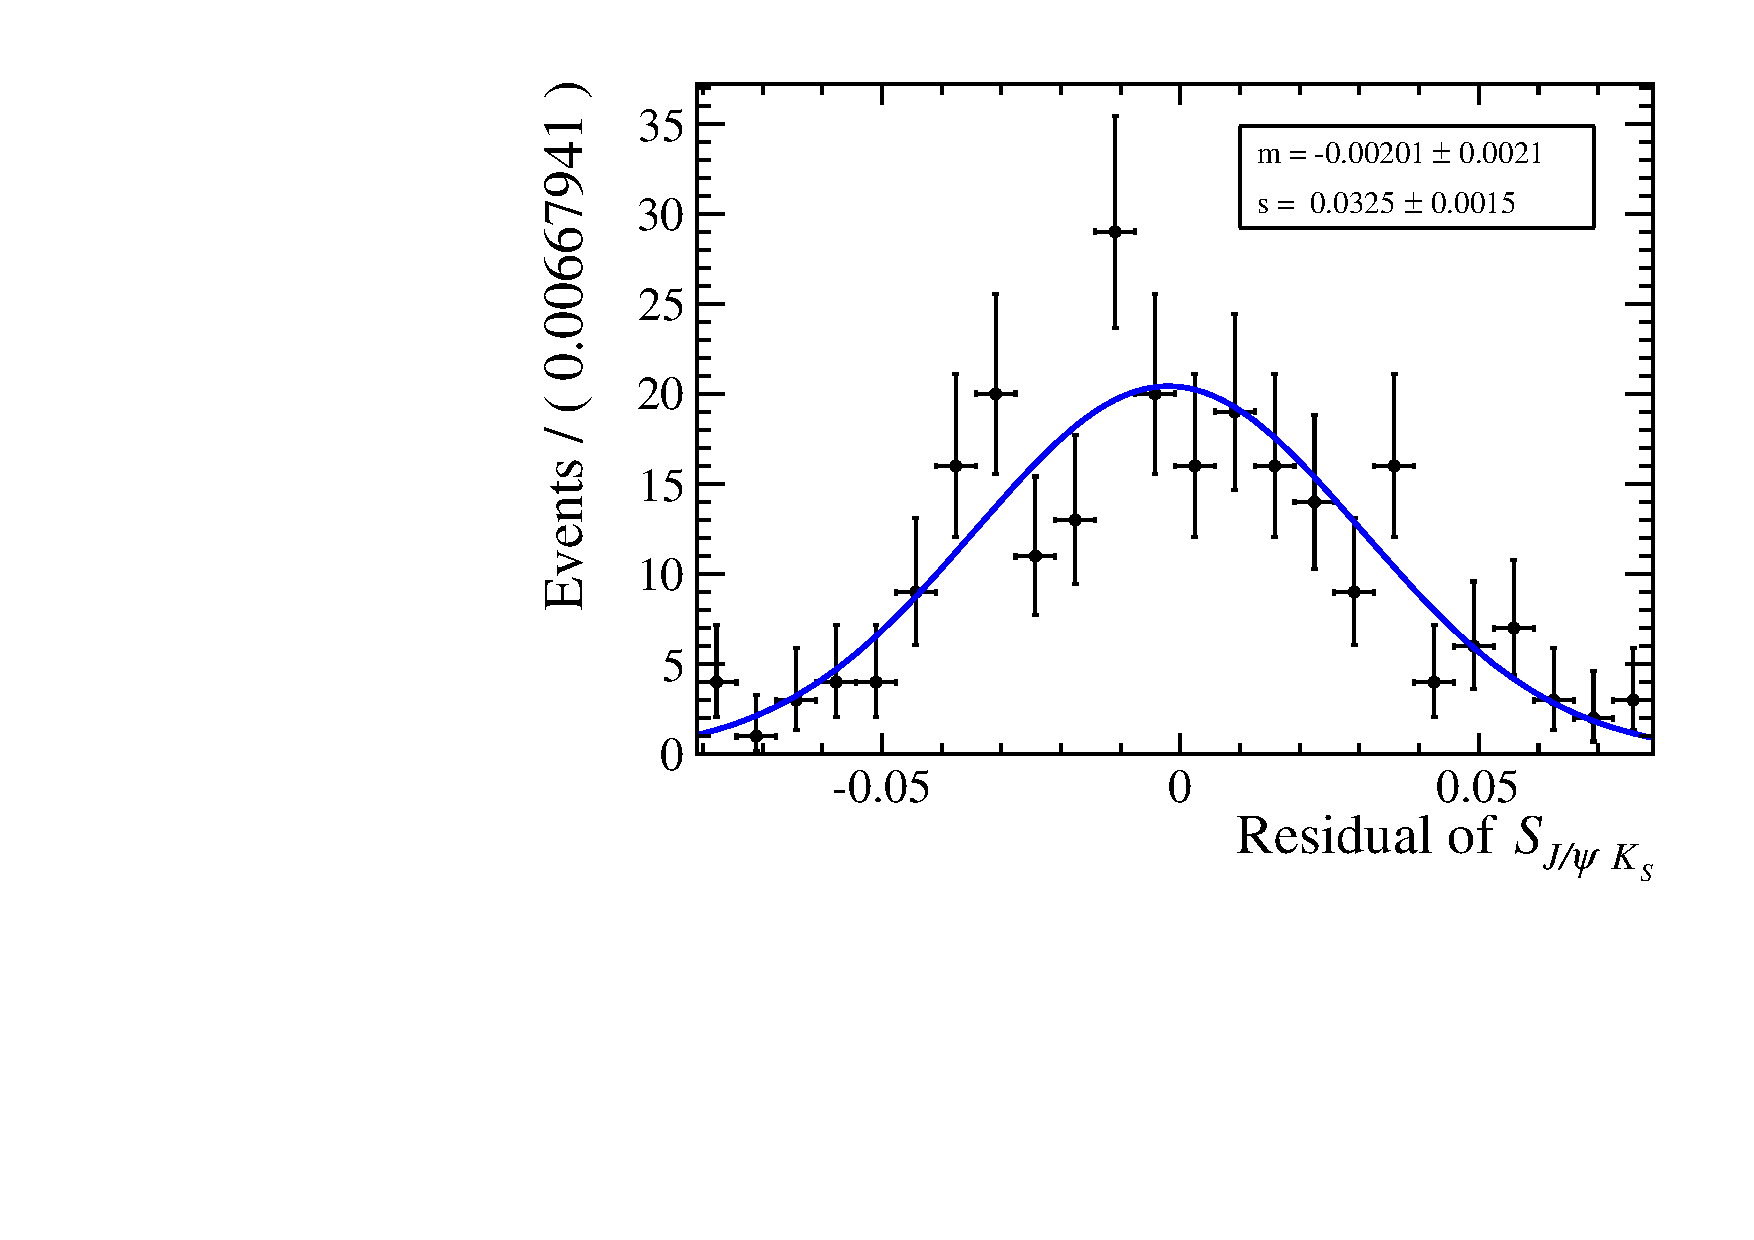
\includegraphics[width=0.49\textwidth]{private/content/appendices/figs/systematics_acc_lower_s_res.pdf}
  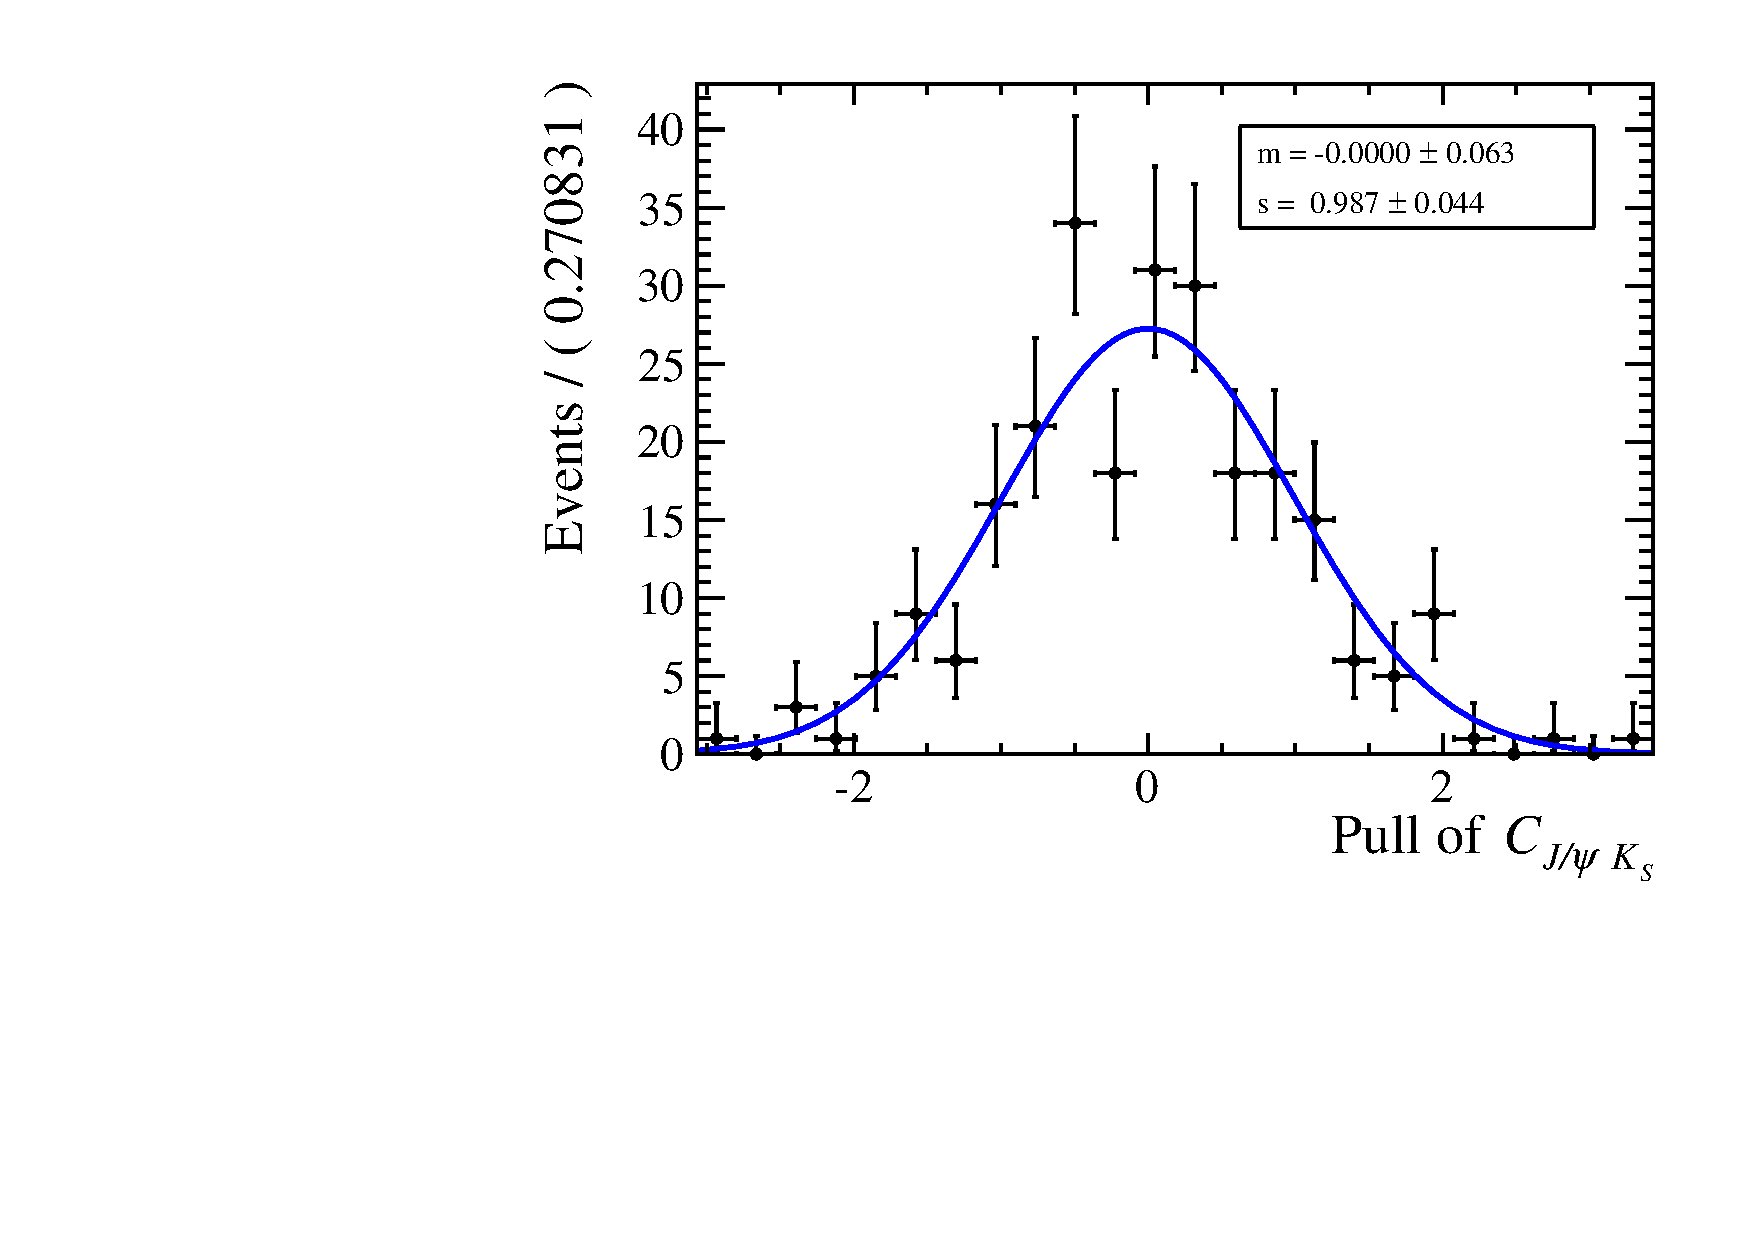
\includegraphics[width=0.49\textwidth]{private/content/appendices/figs/systematics_acc_lower_c_pull.pdf}\hfill
  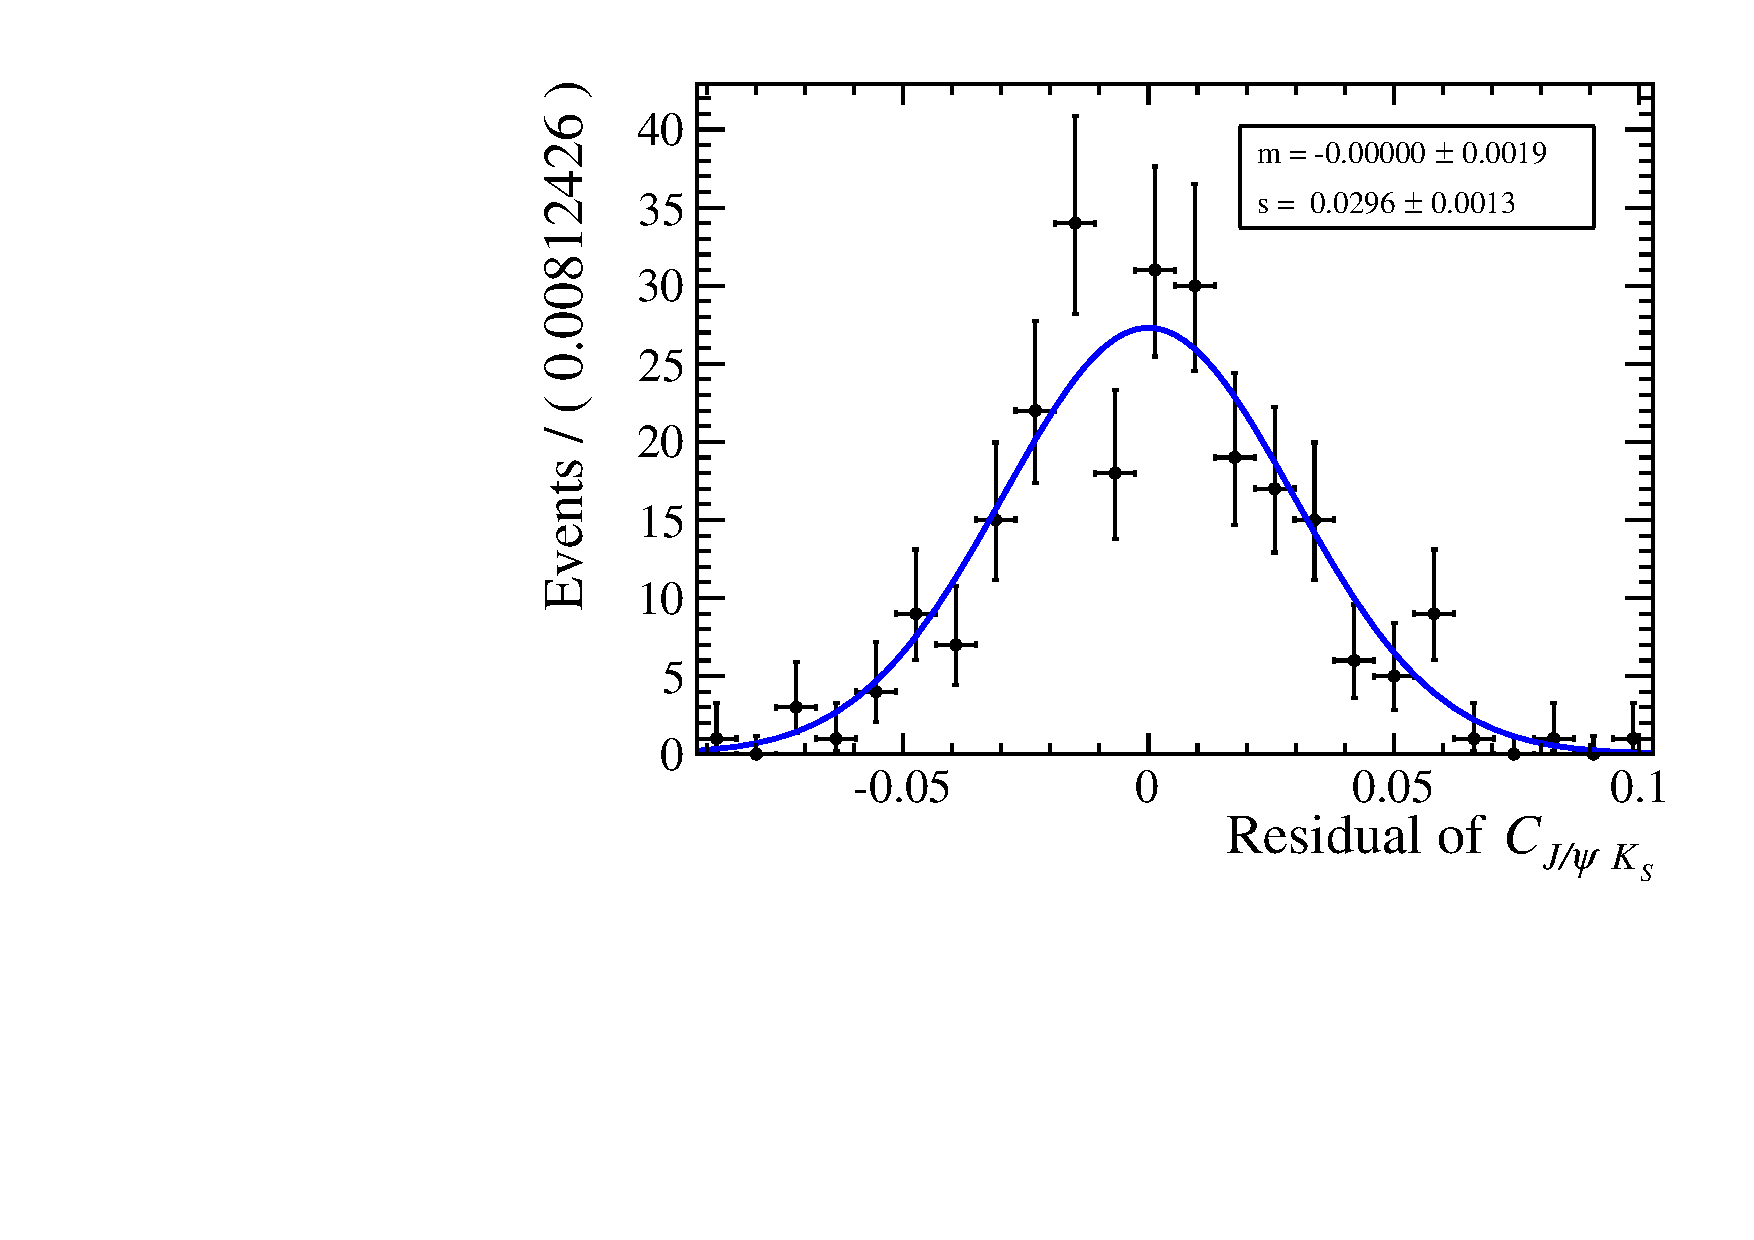
\includegraphics[width=0.49\textwidth]{private/content/appendices/figs/systematics_acc_lower_c_res.pdf}
\caption{Shown are (left) pull and (right) residual distributions of the
parameters (top) \SJpsiKS and (bottom) \CJpsiKS from a \ToyMC study of the
influence of the low decay time acceptance model on the measurement of the \CP
parameters.}
\label{fig:app:measurement_of_sin2beta:systematics:systematics:acceptance:lower}
\end{figure}

\begin{figure}[h]
  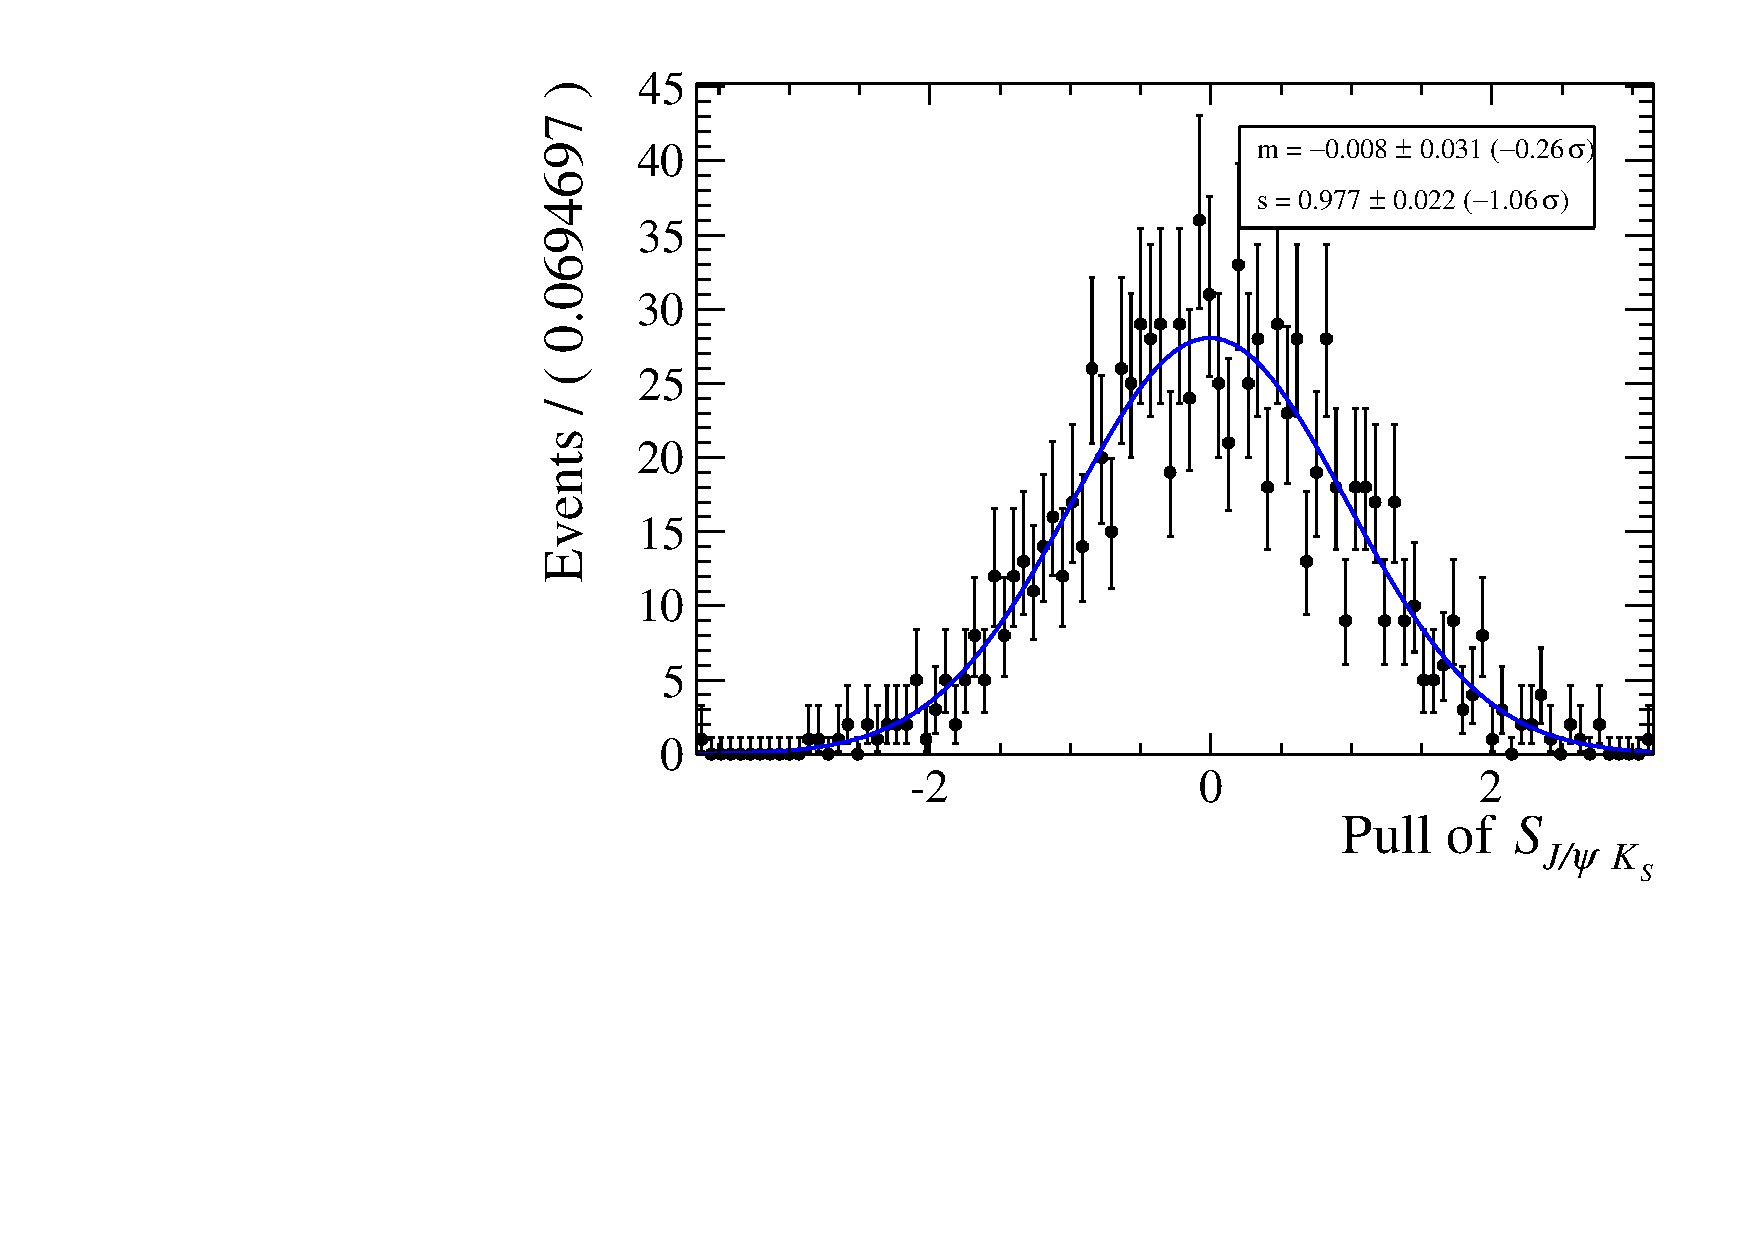
\includegraphics[width=0.49\textwidth]{private/content/appendices/figs/systematics_acc_upper_s_pull.pdf}\hfill
  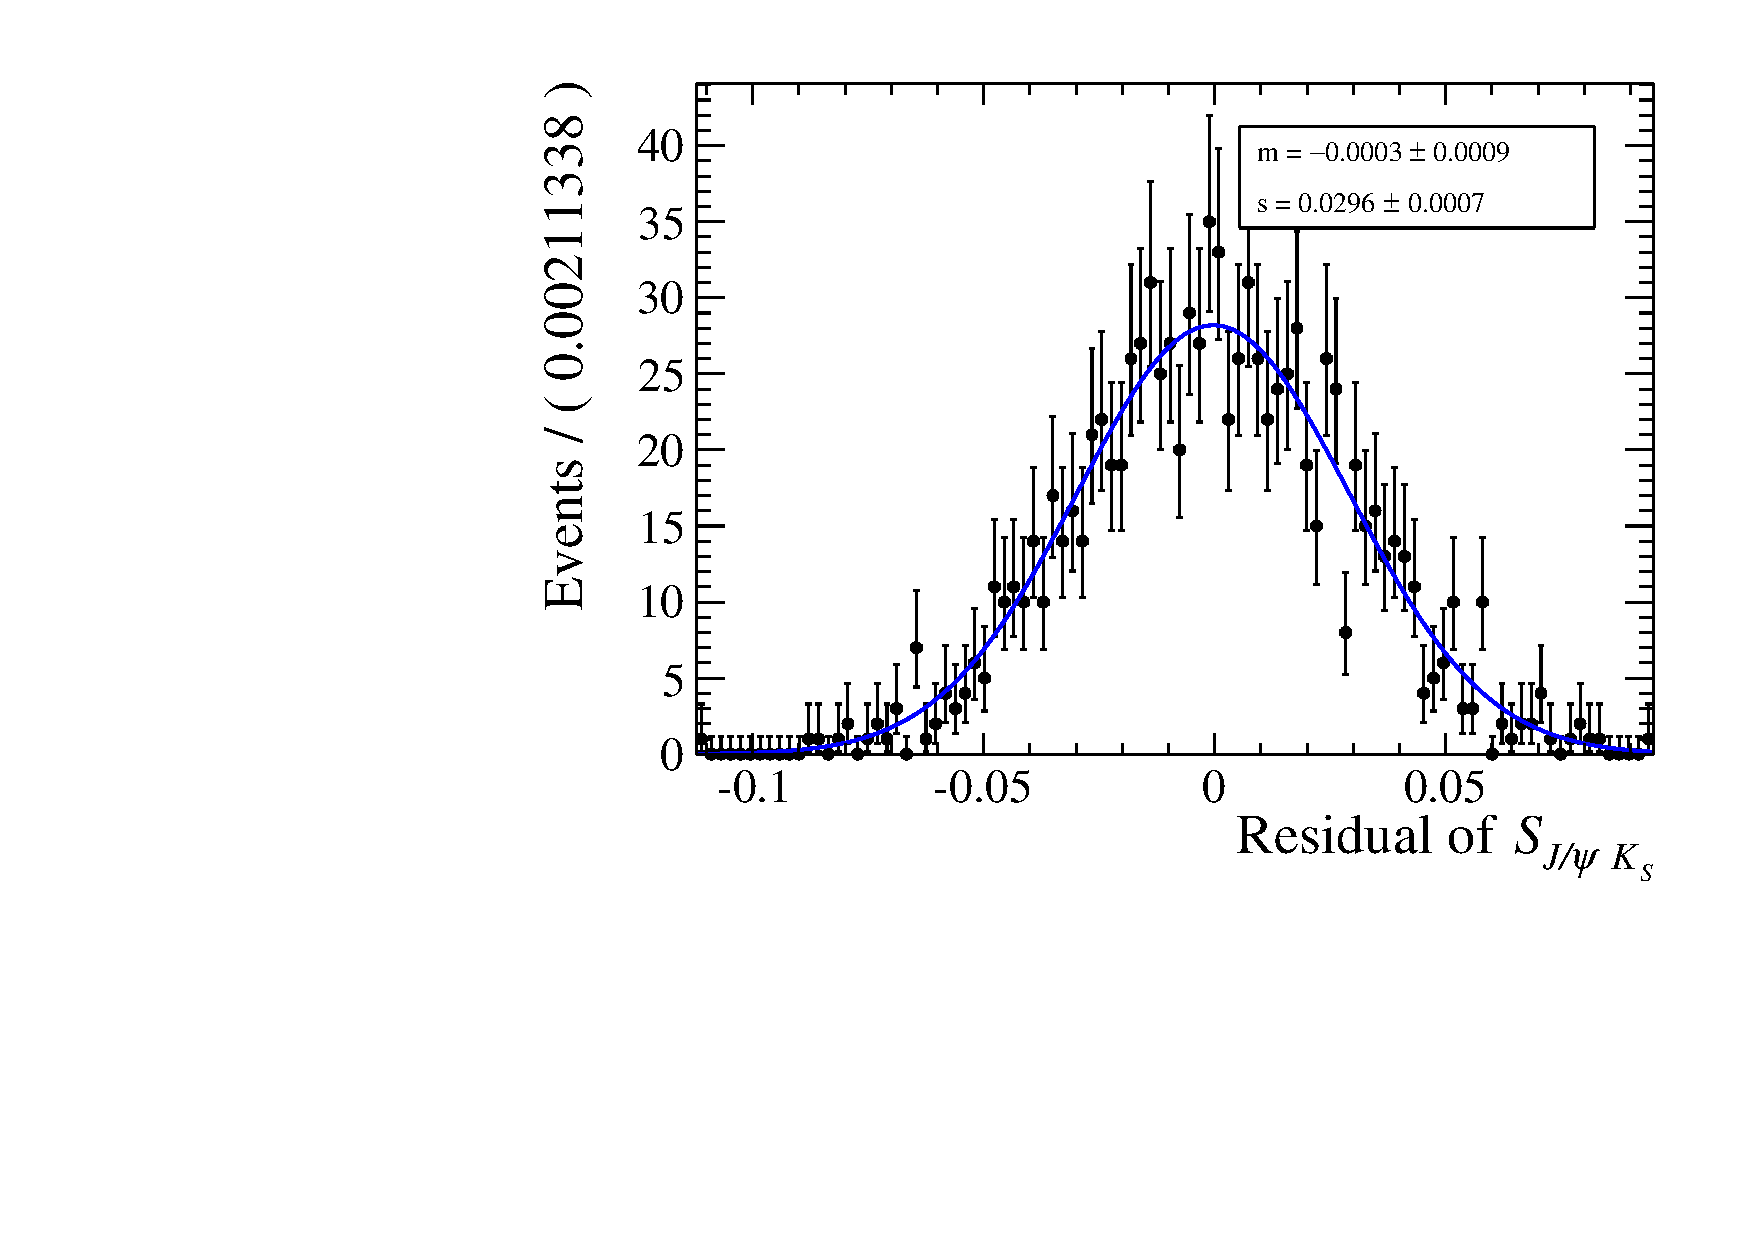
\includegraphics[width=0.49\textwidth]{private/content/appendices/figs/systematics_acc_upper_s_res.pdf}
  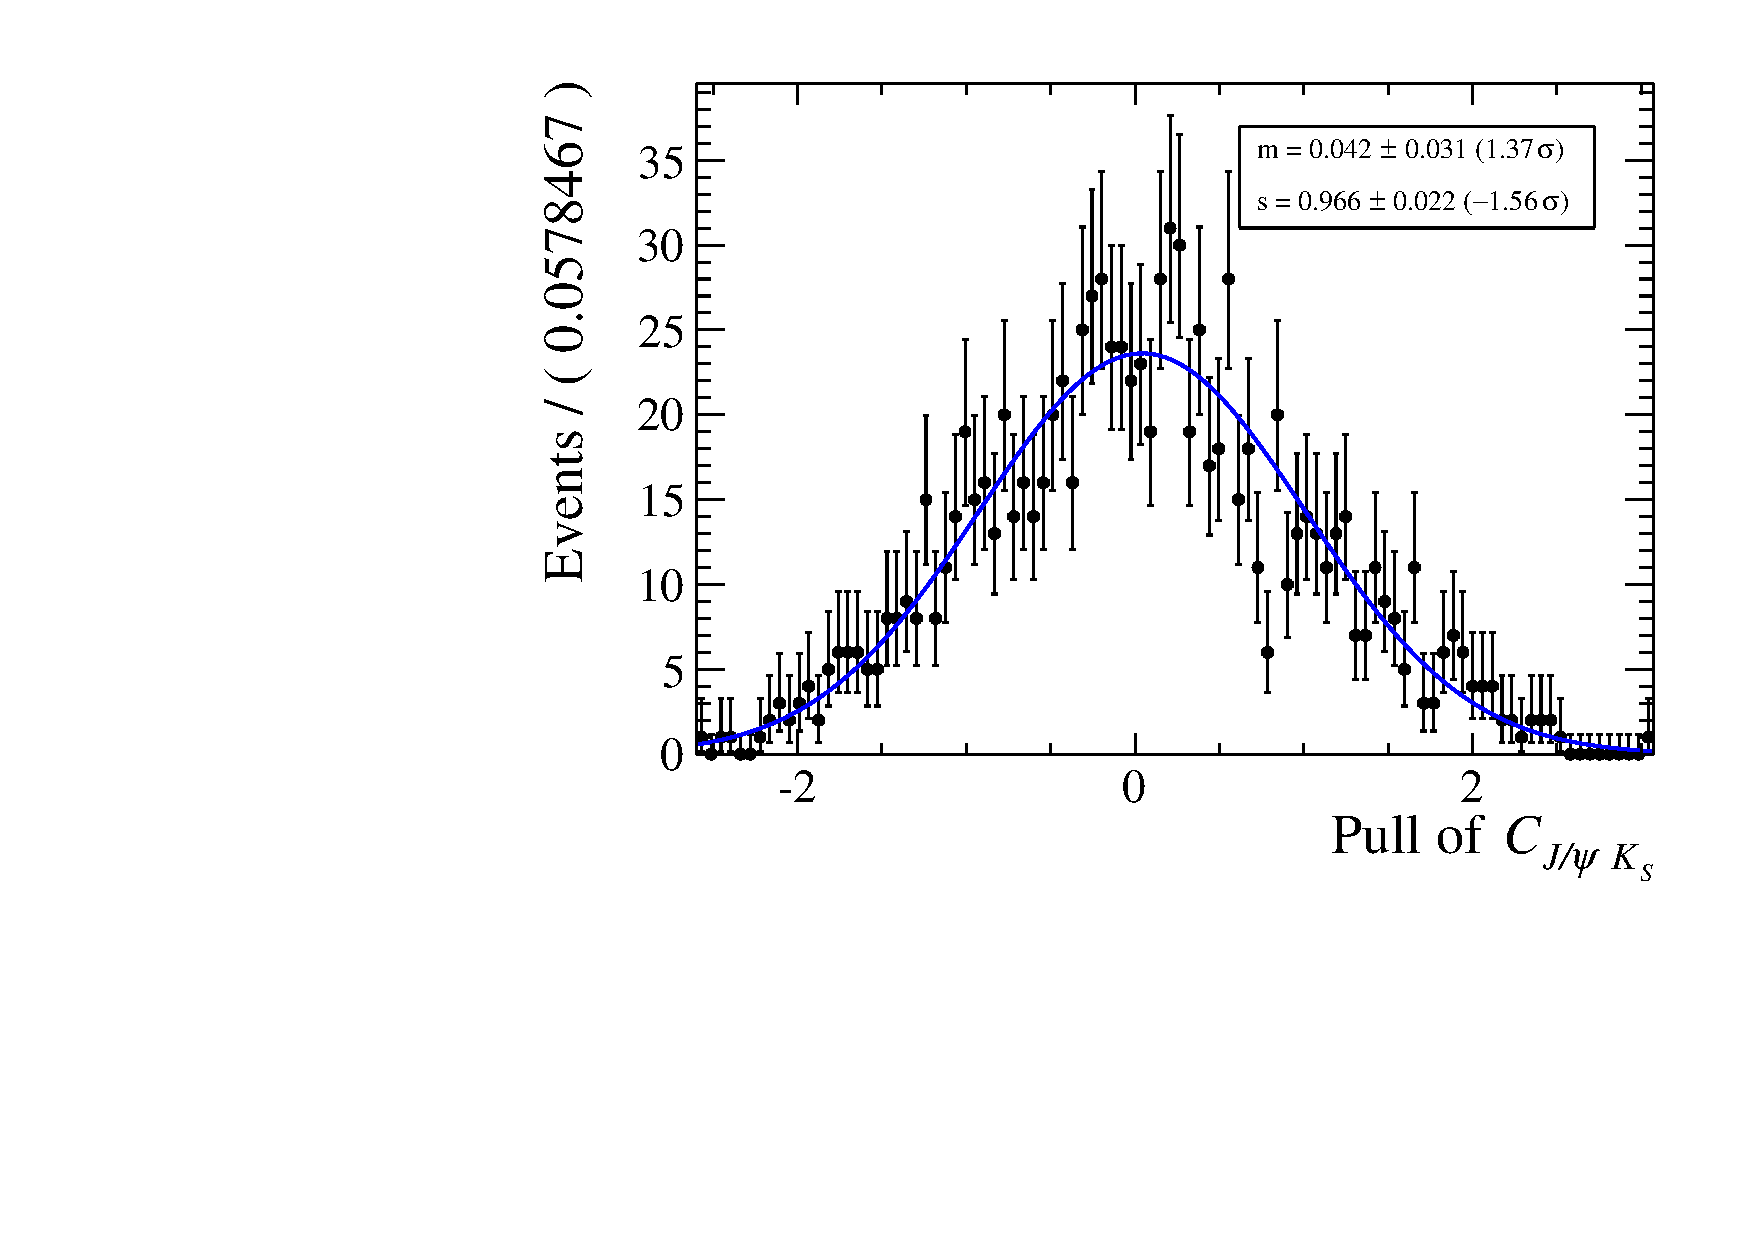
\includegraphics[width=0.49\textwidth]{private/content/appendices/figs/systematics_acc_upper_c_pull.pdf}\hfill
  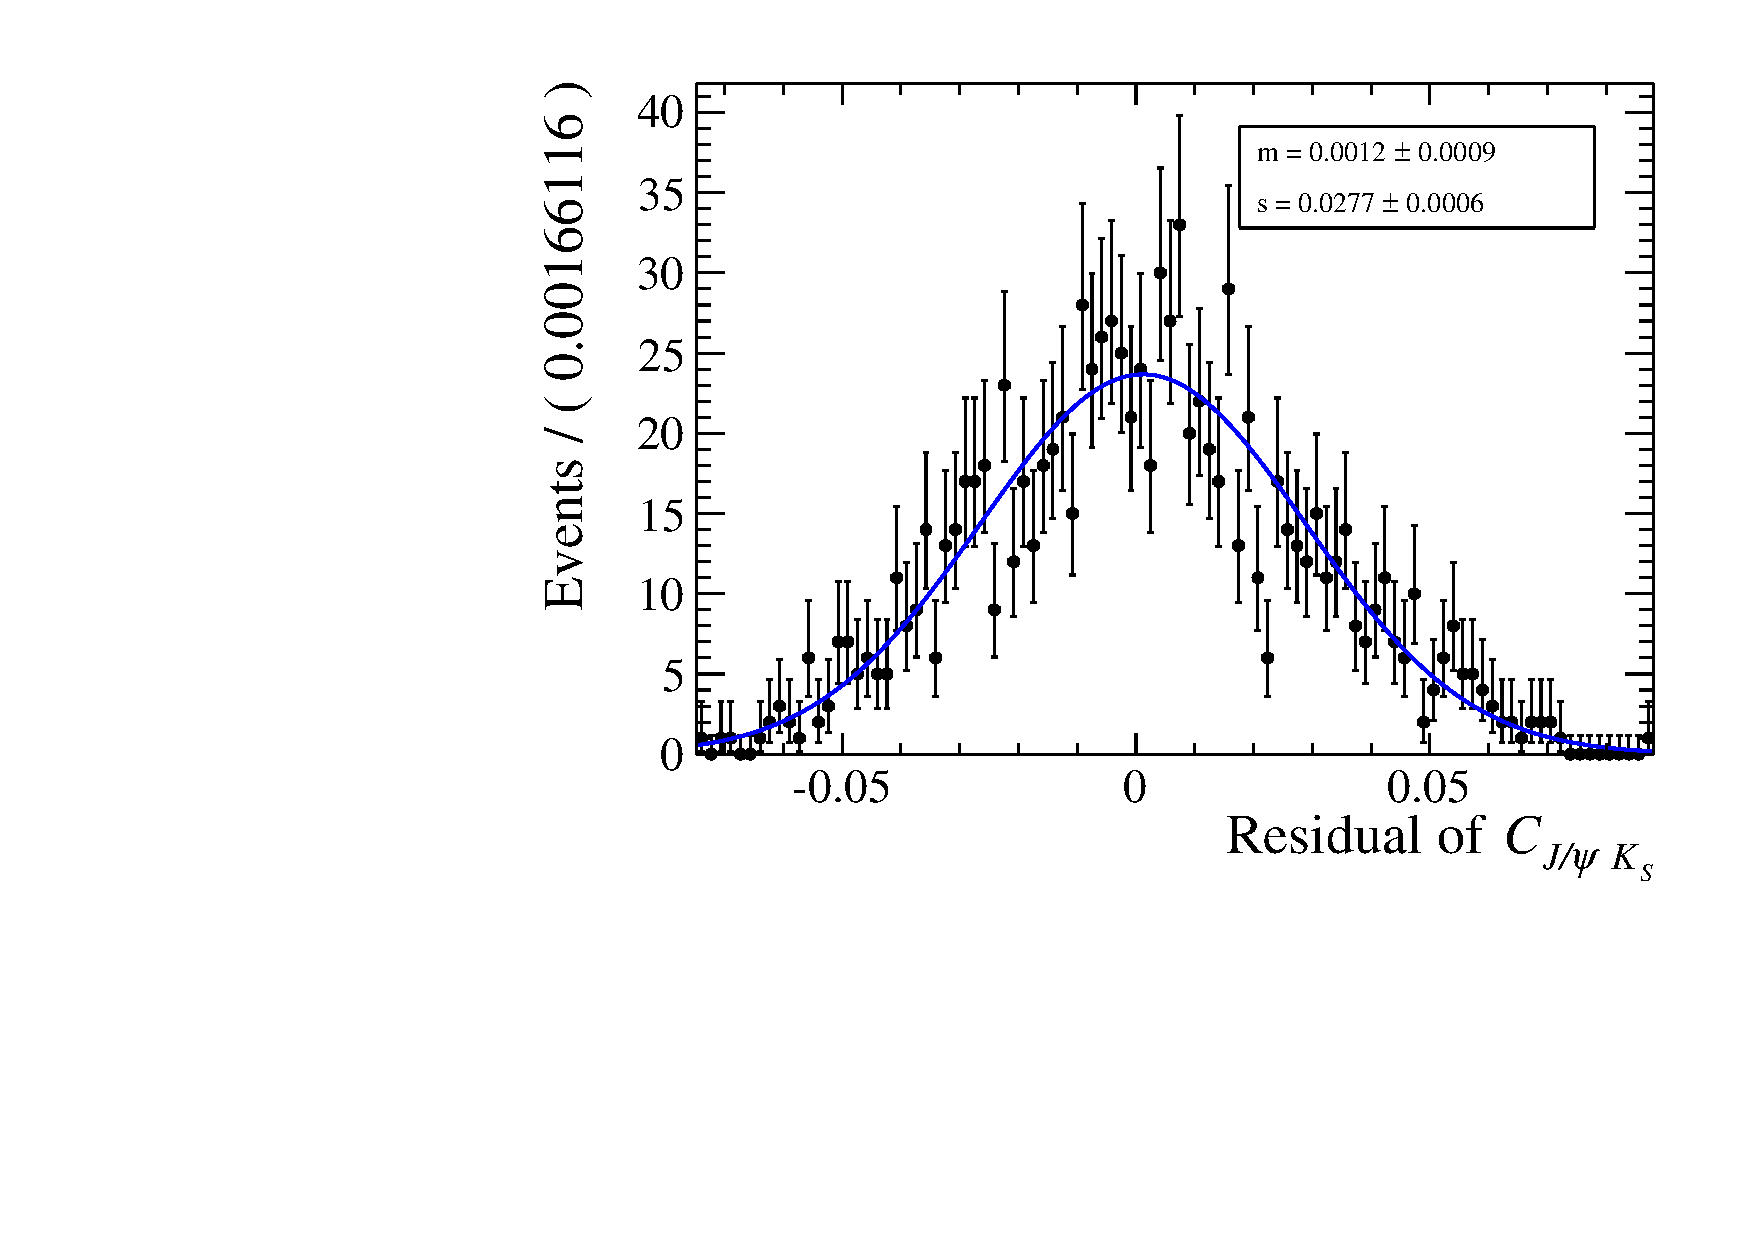
\includegraphics[width=0.49\textwidth]{private/content/appendices/figs/systematics_acc_upper_c_res.pdf}
\caption{Shown are (left) pull and (right) residual distributions of the
parameters (top) \SJpsiKS and (bottom) \CJpsiKS from a \ToyMC study of the
influence of the upper decay time acceptance correction function on the
measurement of the \CP parameters.}
\label{fig:app:measurement_of_sin2beta:systematics:systematics:acceptance:upper}
\end{figure}

\clearpage
% ..............................................................................
\subsubsection[Production asymmetry, $z$-scale, \DMd, and \DGd]{Production asymmetry, $\mathbfsfit{z}$-scale, $\mathbfsfit{\DMd}$, and $\mathbfsfit{\DGd}$}
\label{sec:app:measurement_of_sin2beta:systematics:systematics:further_studies}

\begin{figure}[h]
  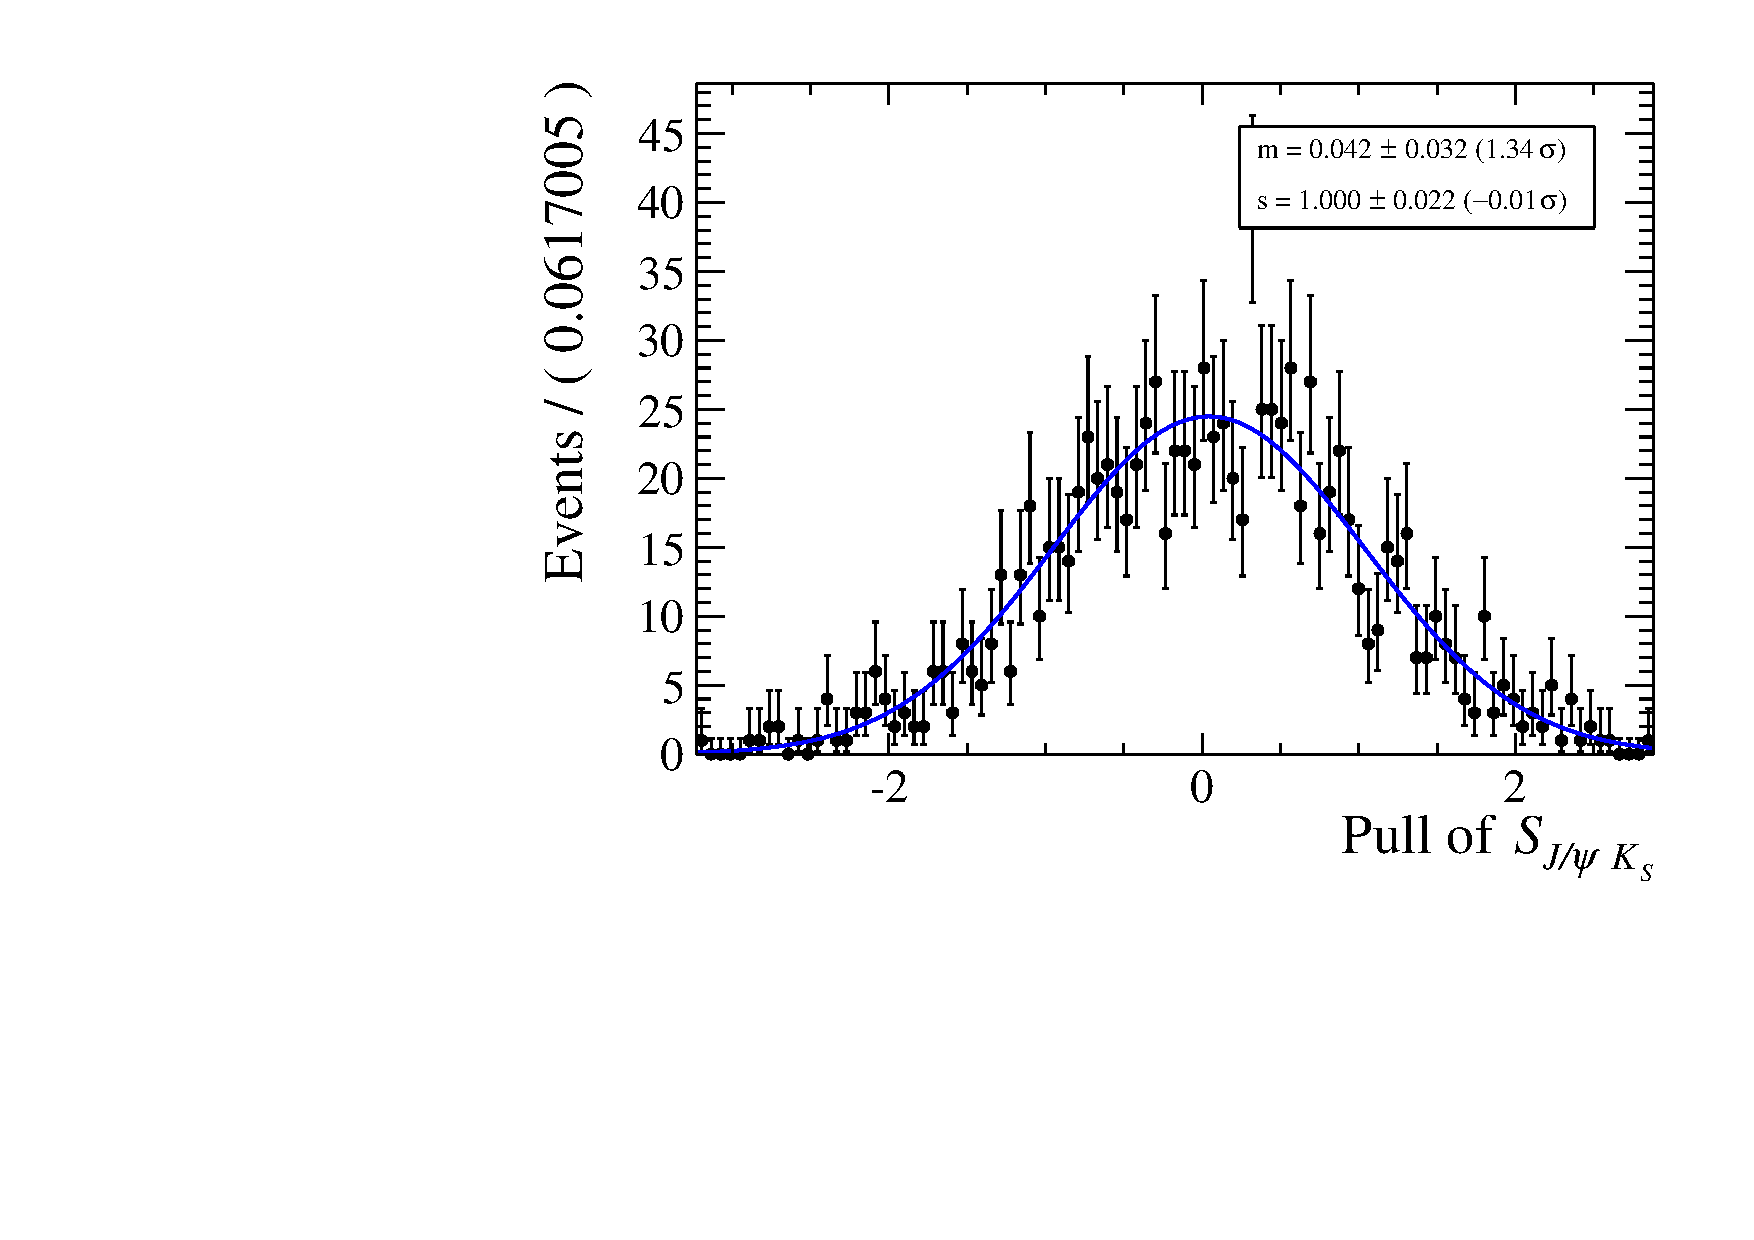
\includegraphics[width=0.49\textwidth]{private/content/appendices/figs/systematics_fs_zscale_s_pull.pdf}\hfill
  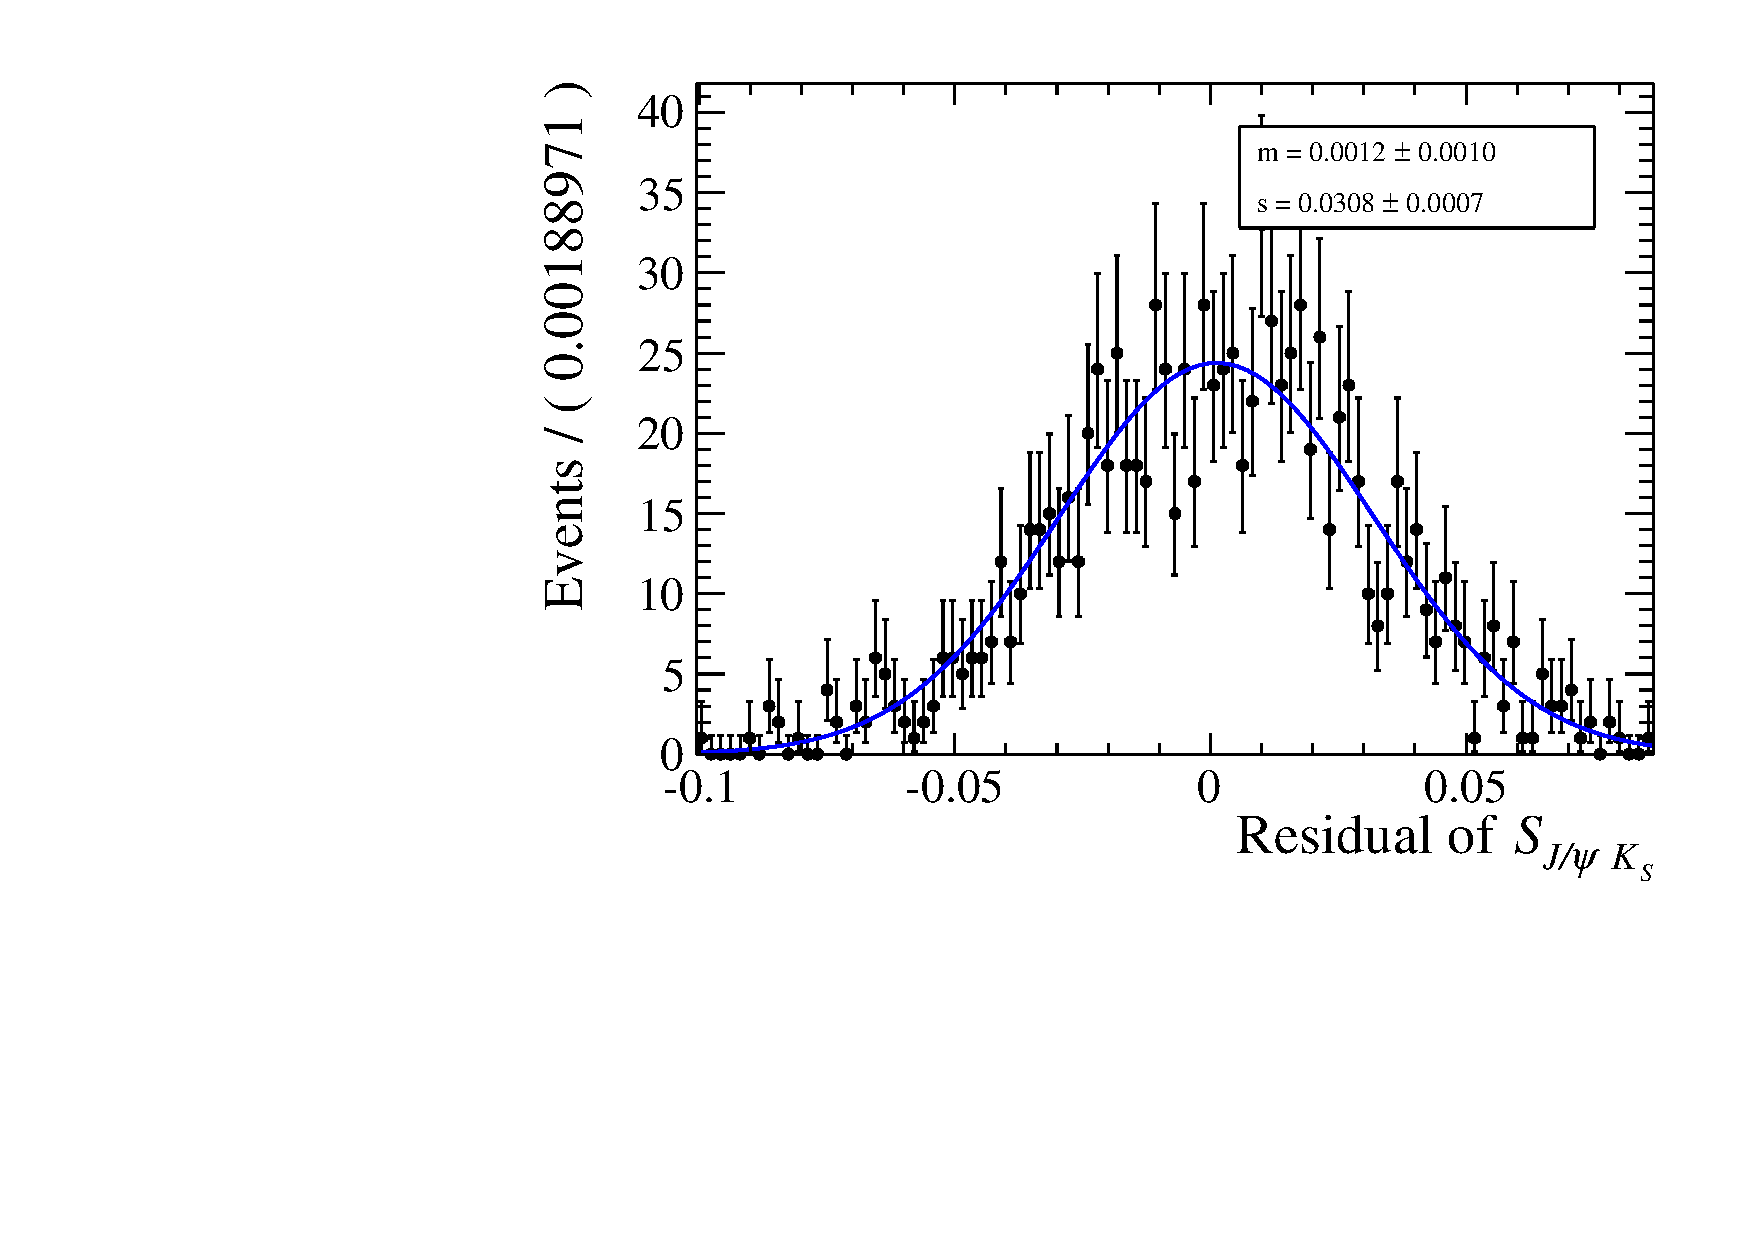
\includegraphics[width=0.49\textwidth]{private/content/appendices/figs/systematics_fs_zscale_s_res.pdf}
  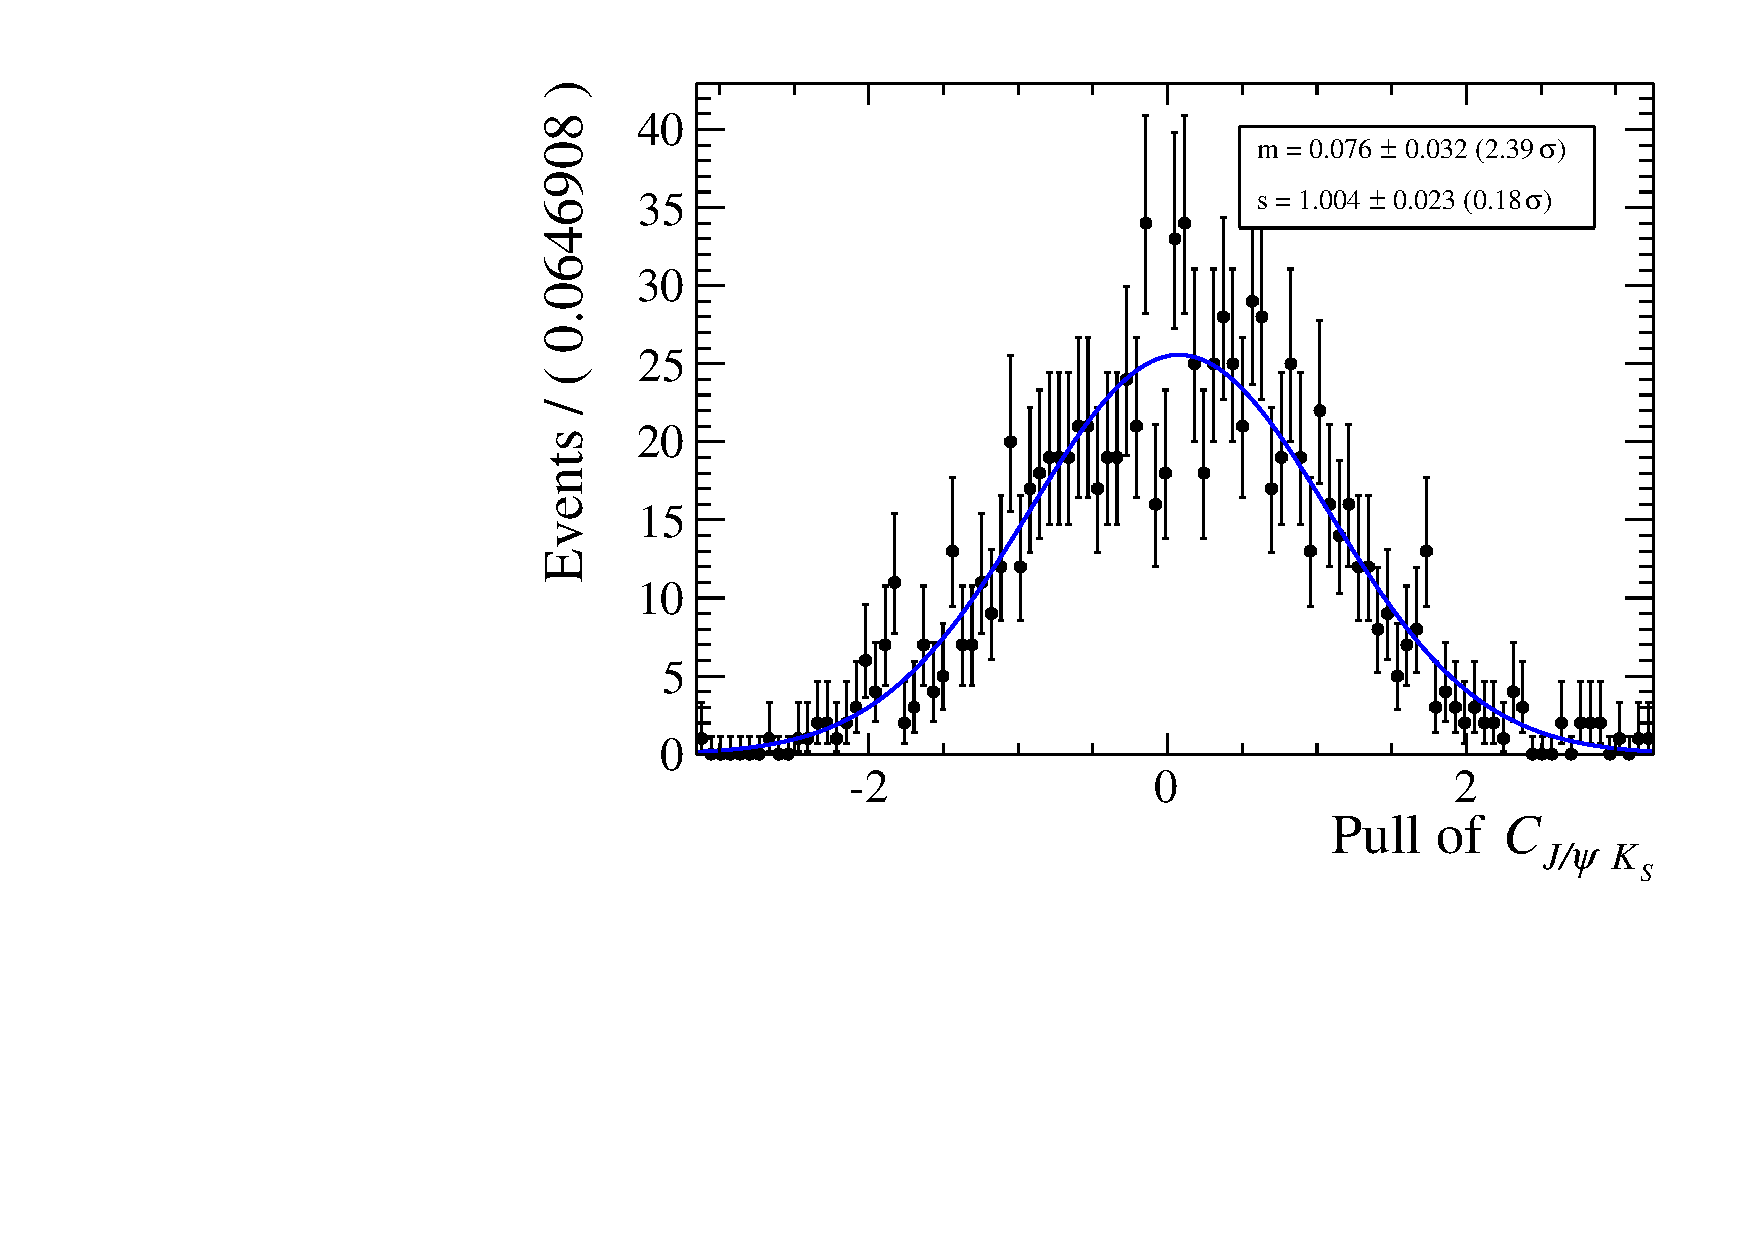
\includegraphics[width=0.49\textwidth]{private/content/appendices/figs/systematics_fs_zscale_c_pull.pdf}\hfill
  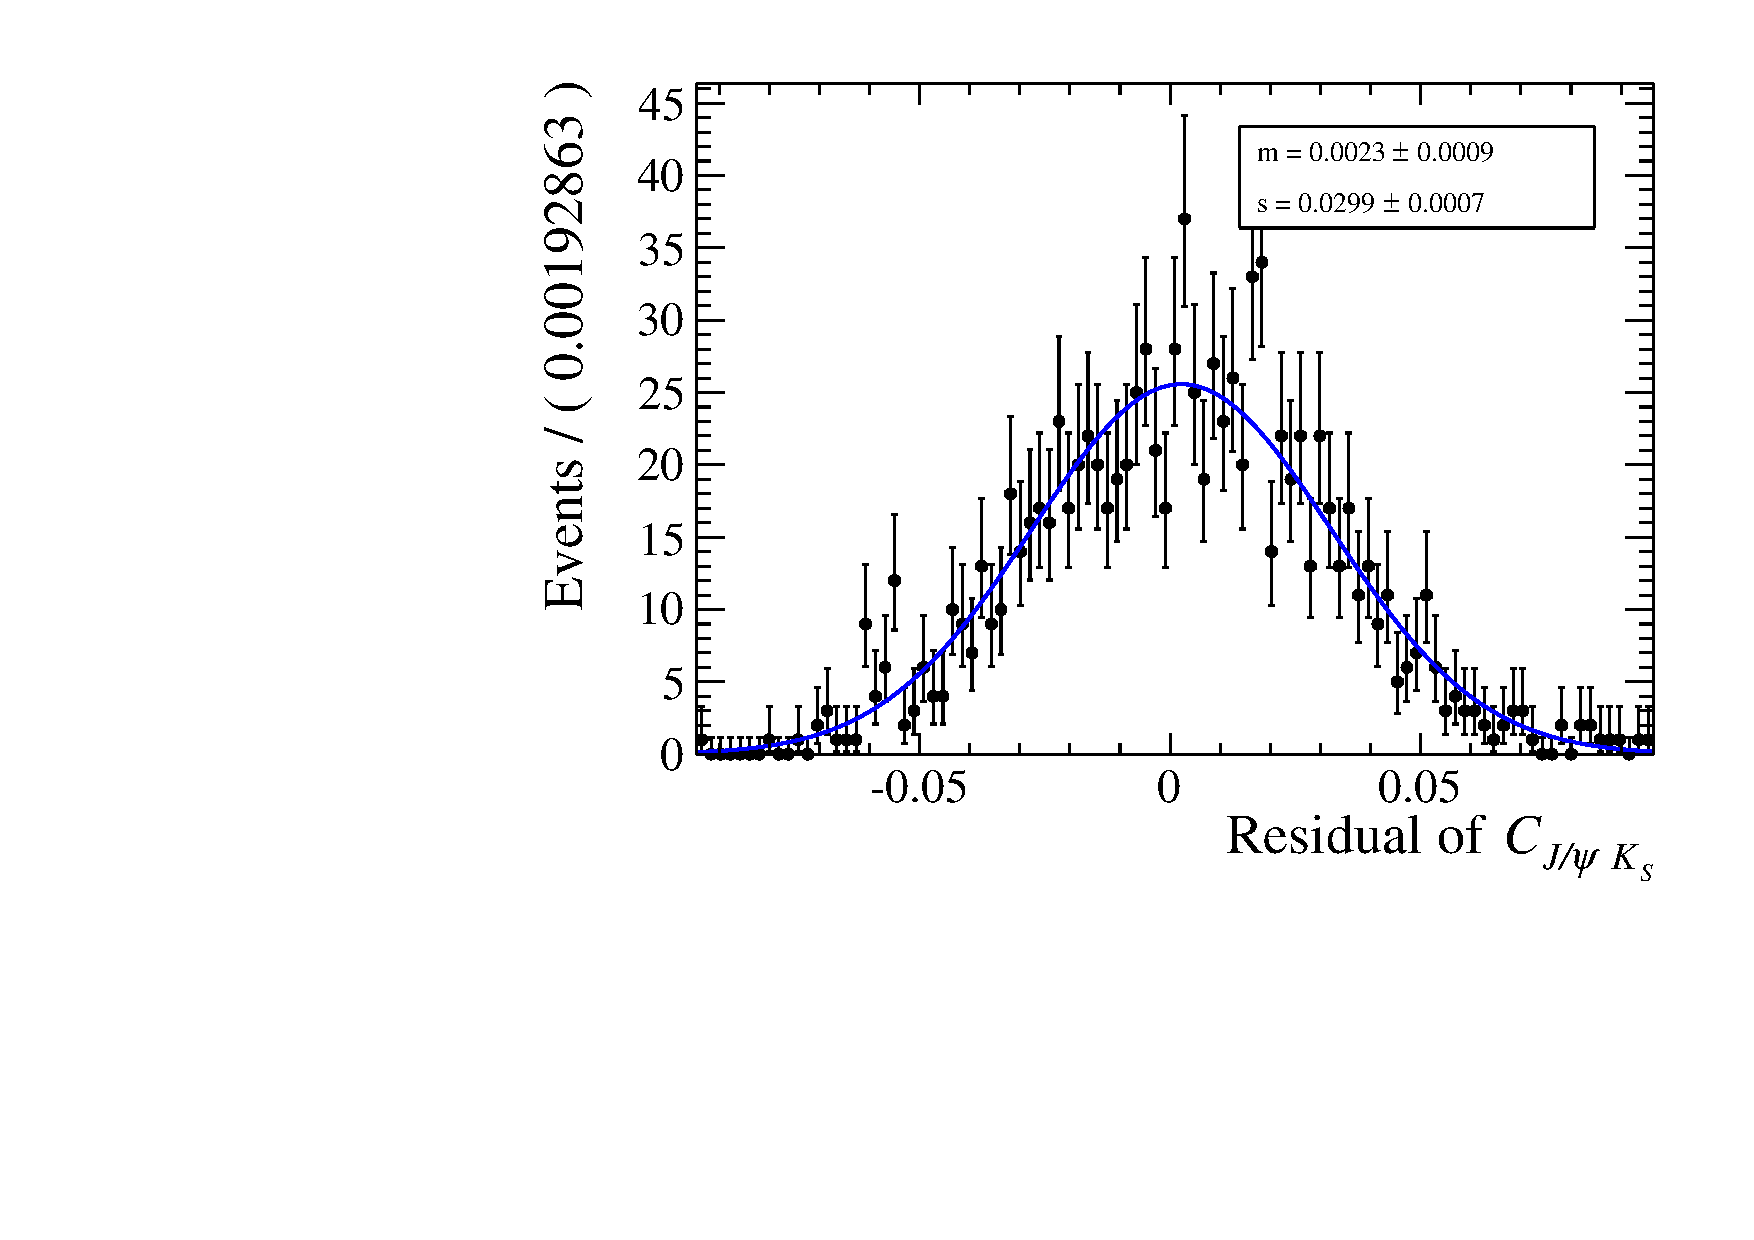
\includegraphics[width=0.49\textwidth]{private/content/appendices/figs/systematics_fs_zscale_c_res.pdf}
\caption{Shown are (left) pull and (right) residual distributions of the
parameters (top) \SJpsiKS and (bottom) \CJpsiKS from a \ToyMC study of the
influence of the relative $z$-scale uncertainty on the measurement of the \CP
parameters.}
\label{fig:app:measurement_of_sin2beta:systematics:systematics:further_studies:zscale}
\end{figure}

\begin{figure}[h]
  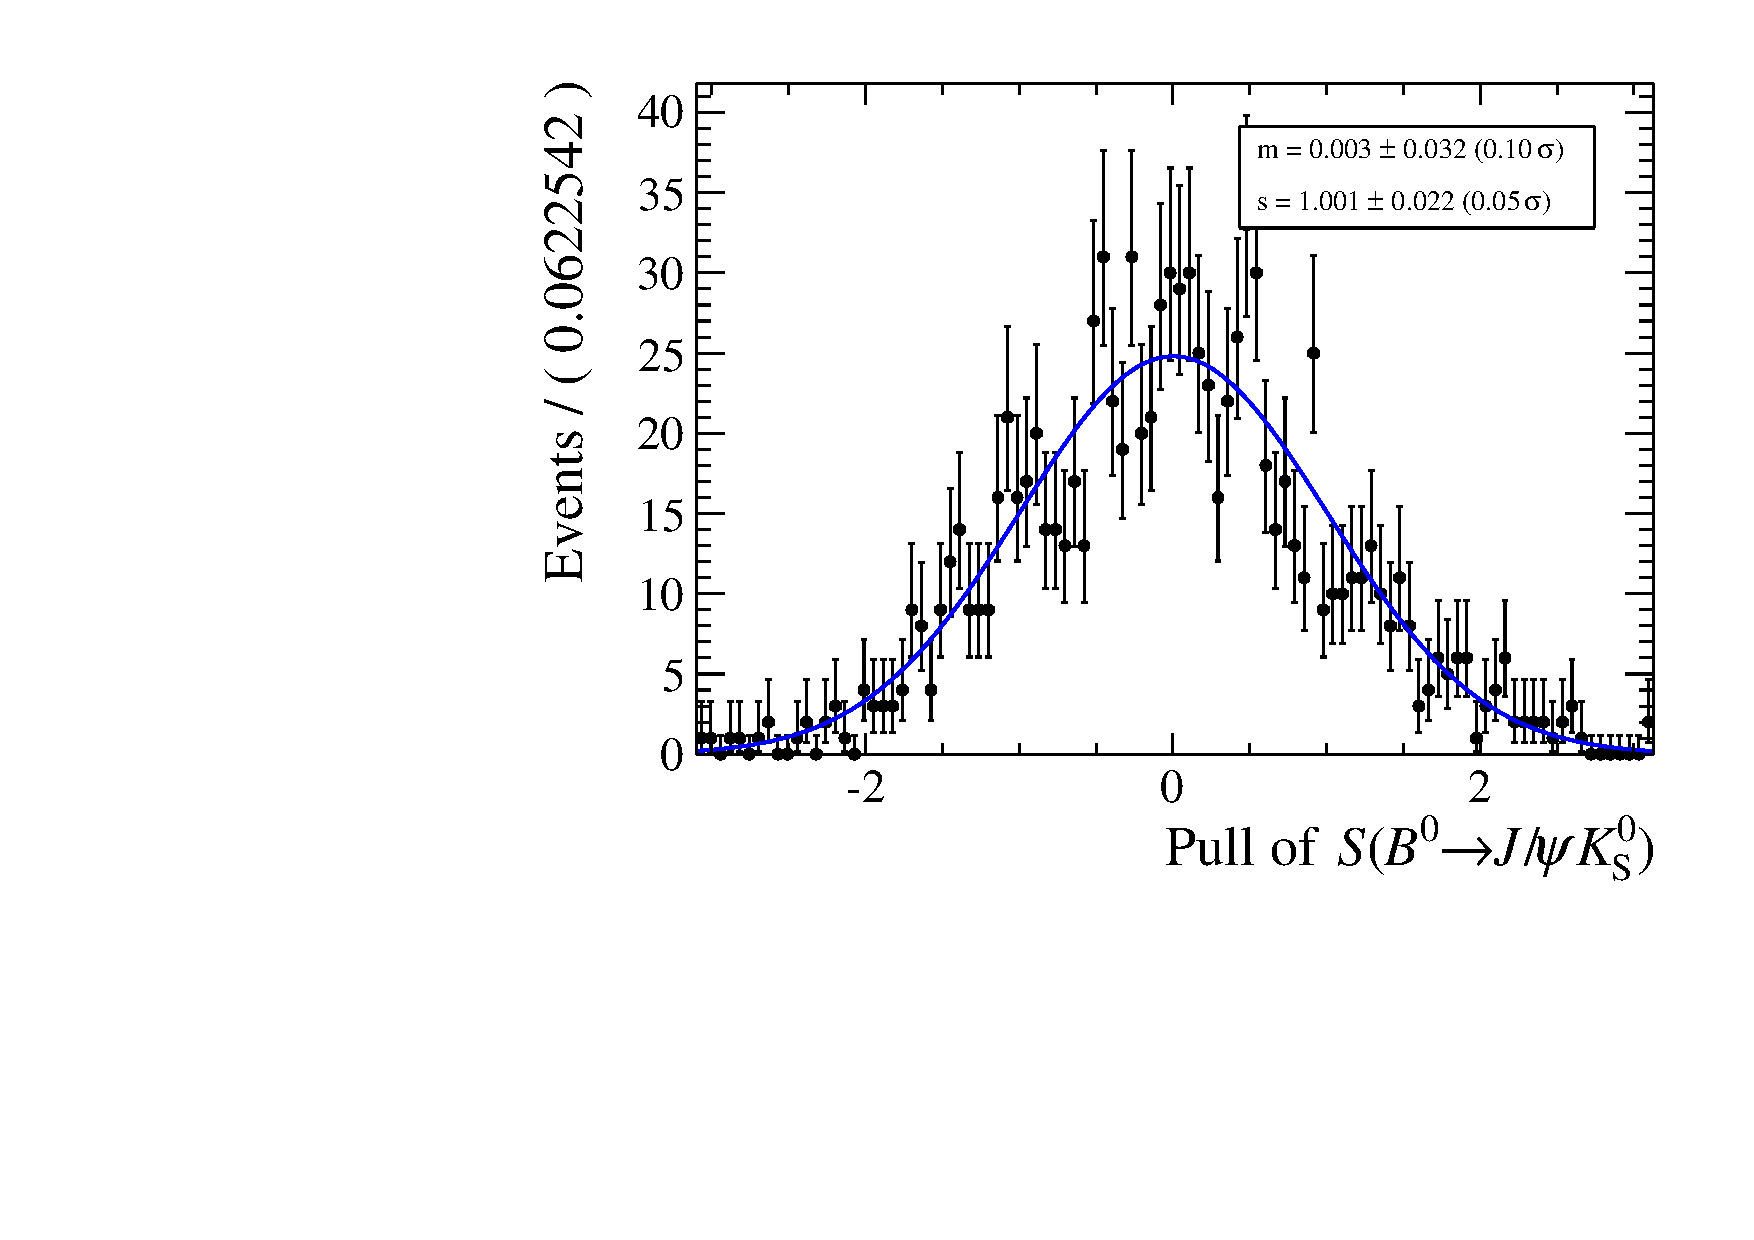
\includegraphics[width=0.49\textwidth]{private/content/appendices/figs/systematics_fs_prodasym_s_pull.pdf}\hfill
  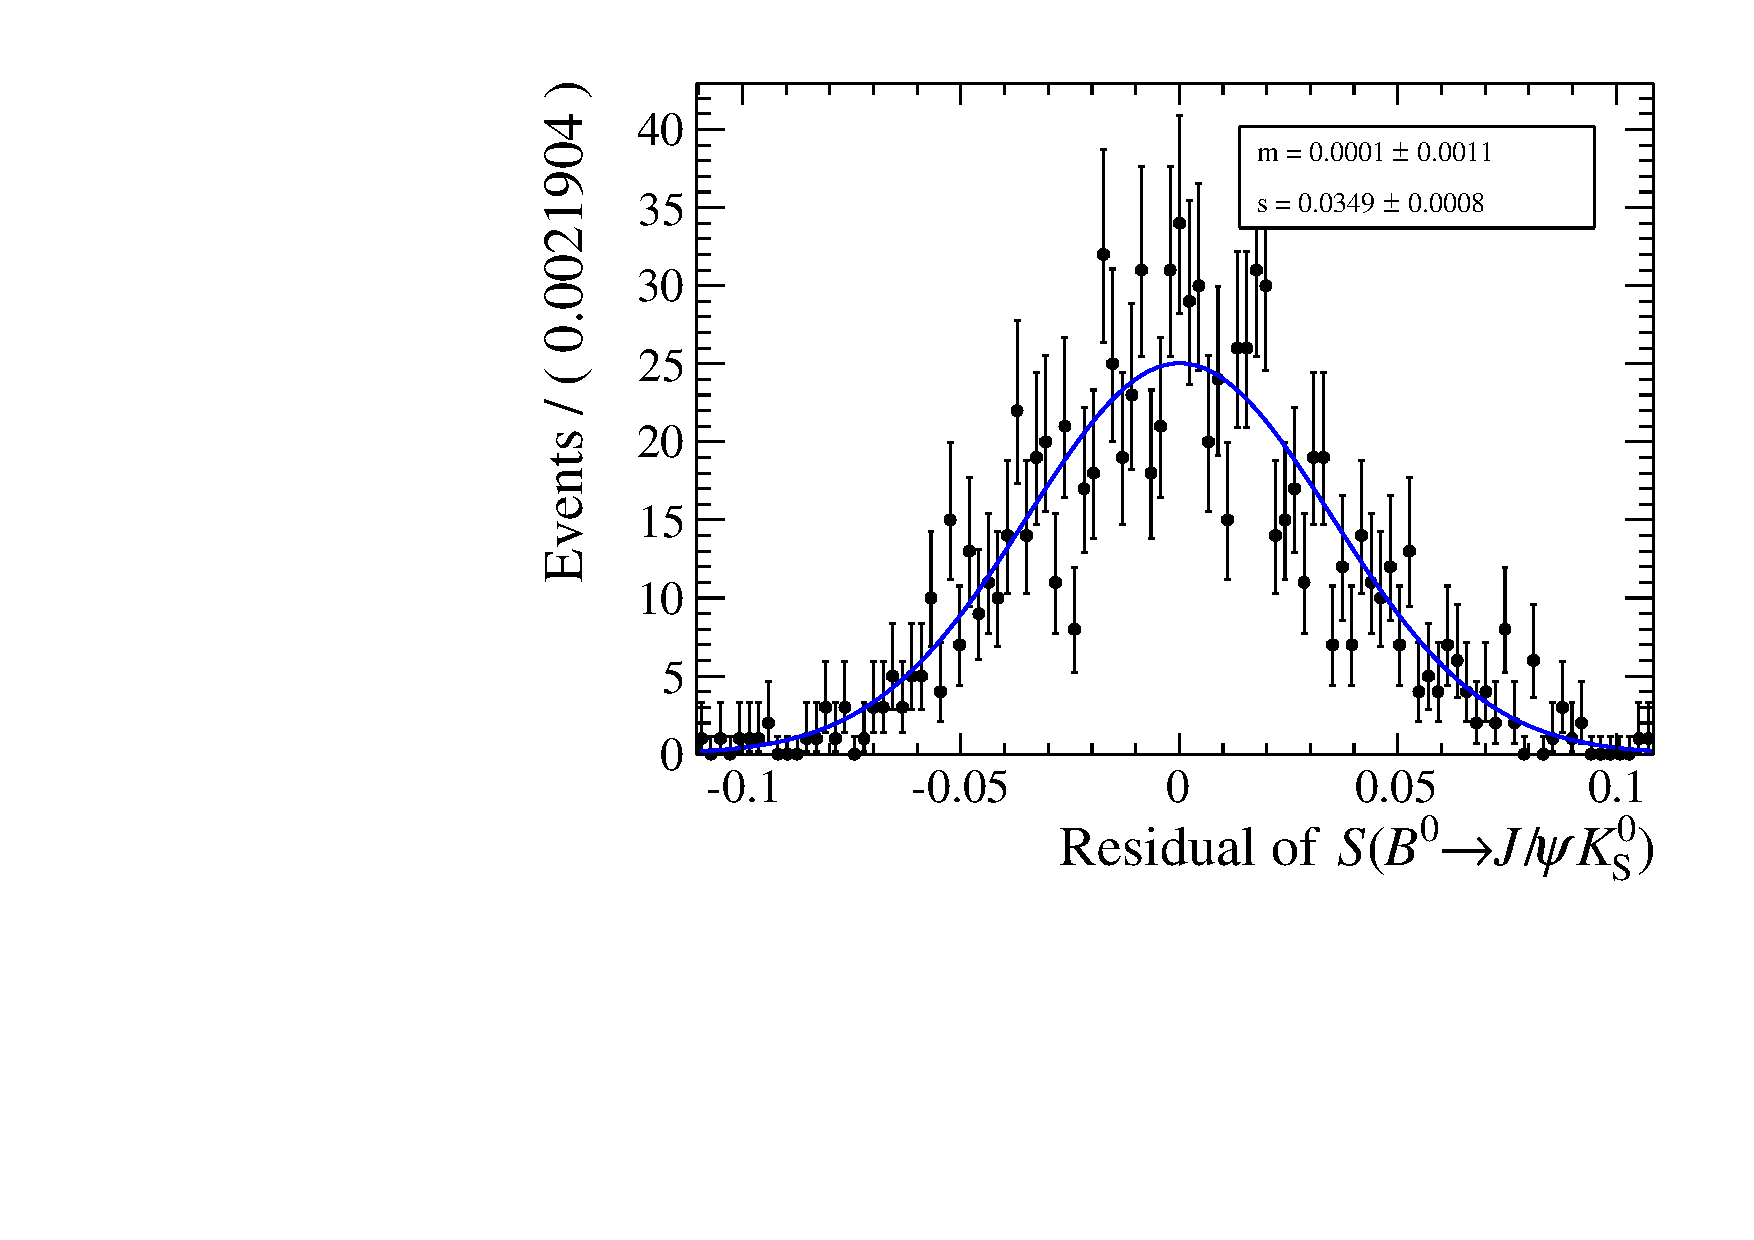
\includegraphics[width=0.49\textwidth]{private/content/appendices/figs/systematics_fs_prodasym_s_res.pdf}
  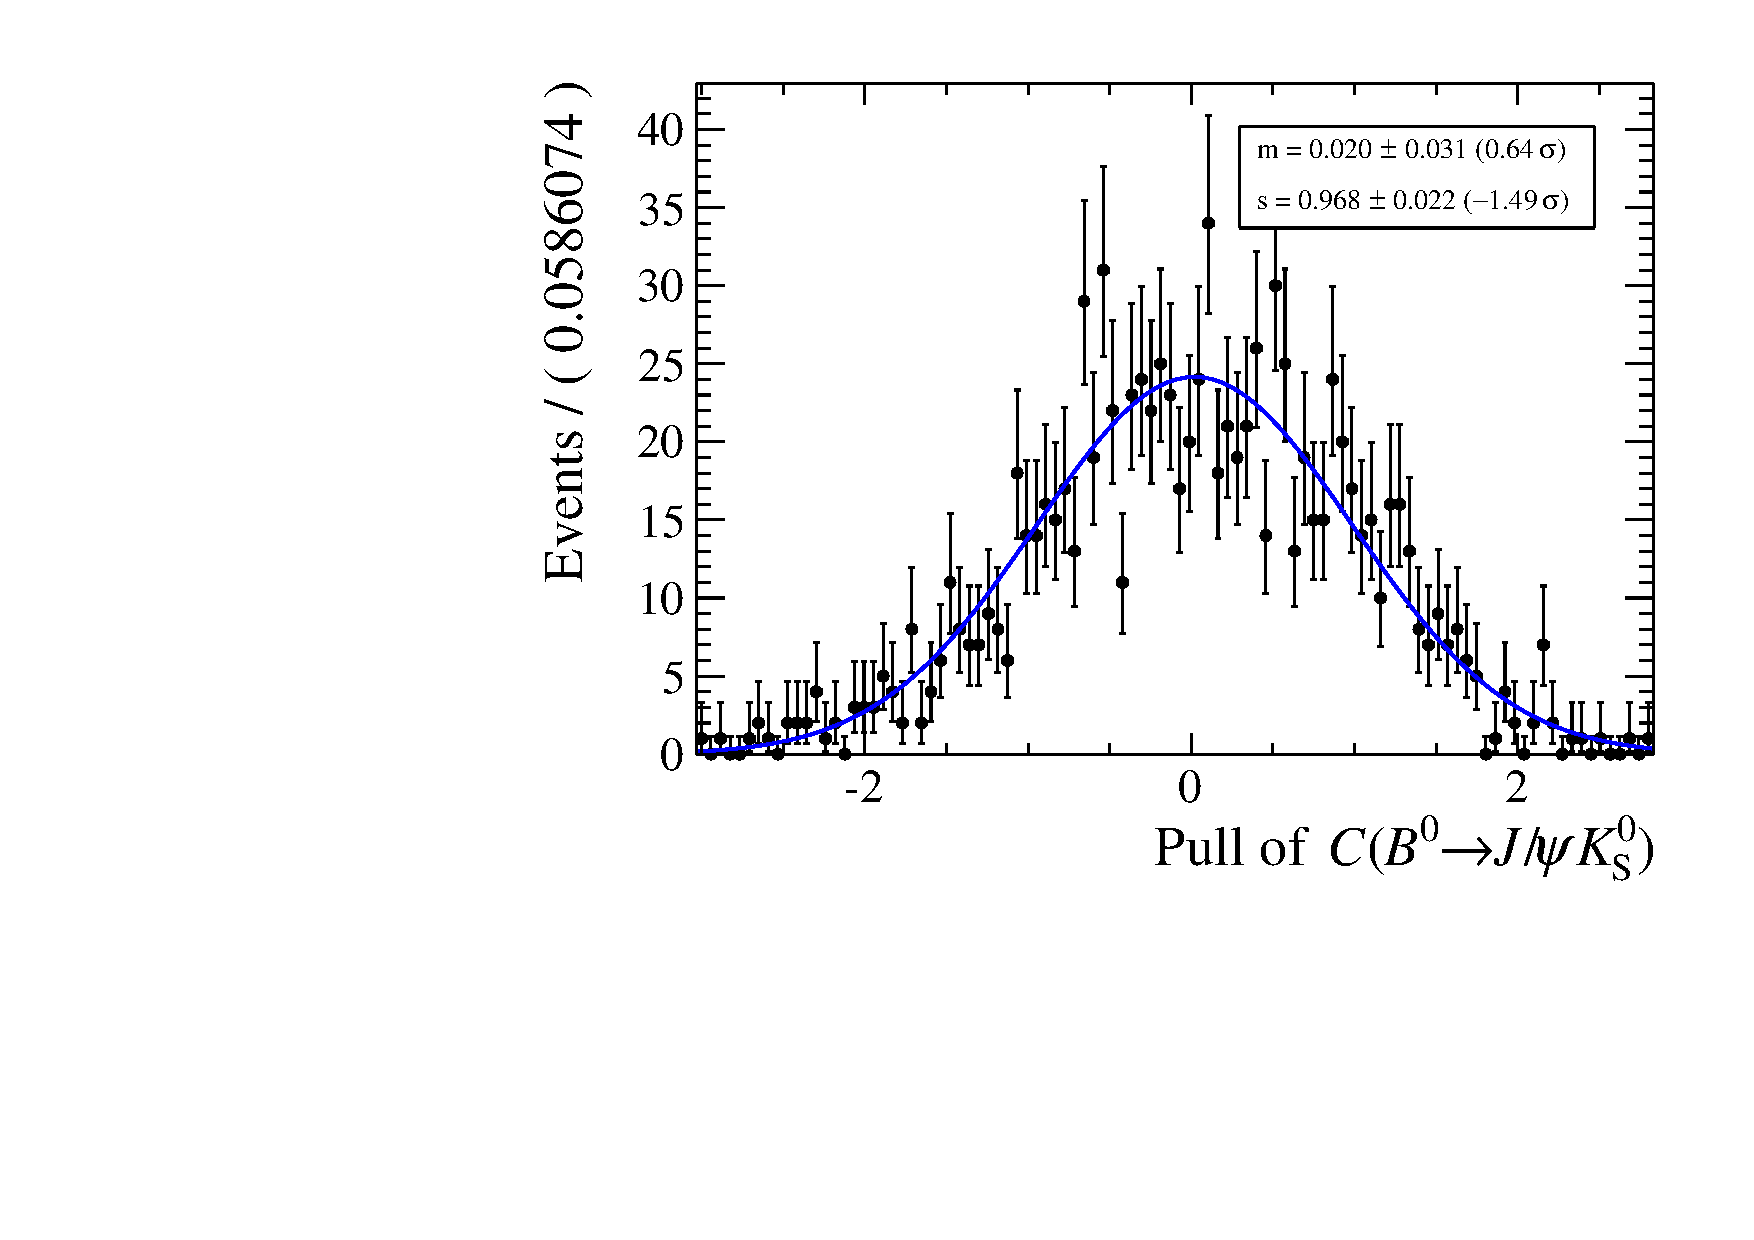
\includegraphics[width=0.49\textwidth]{private/content/appendices/figs/systematics_fs_prodasym_c_pull.pdf}\hfill
  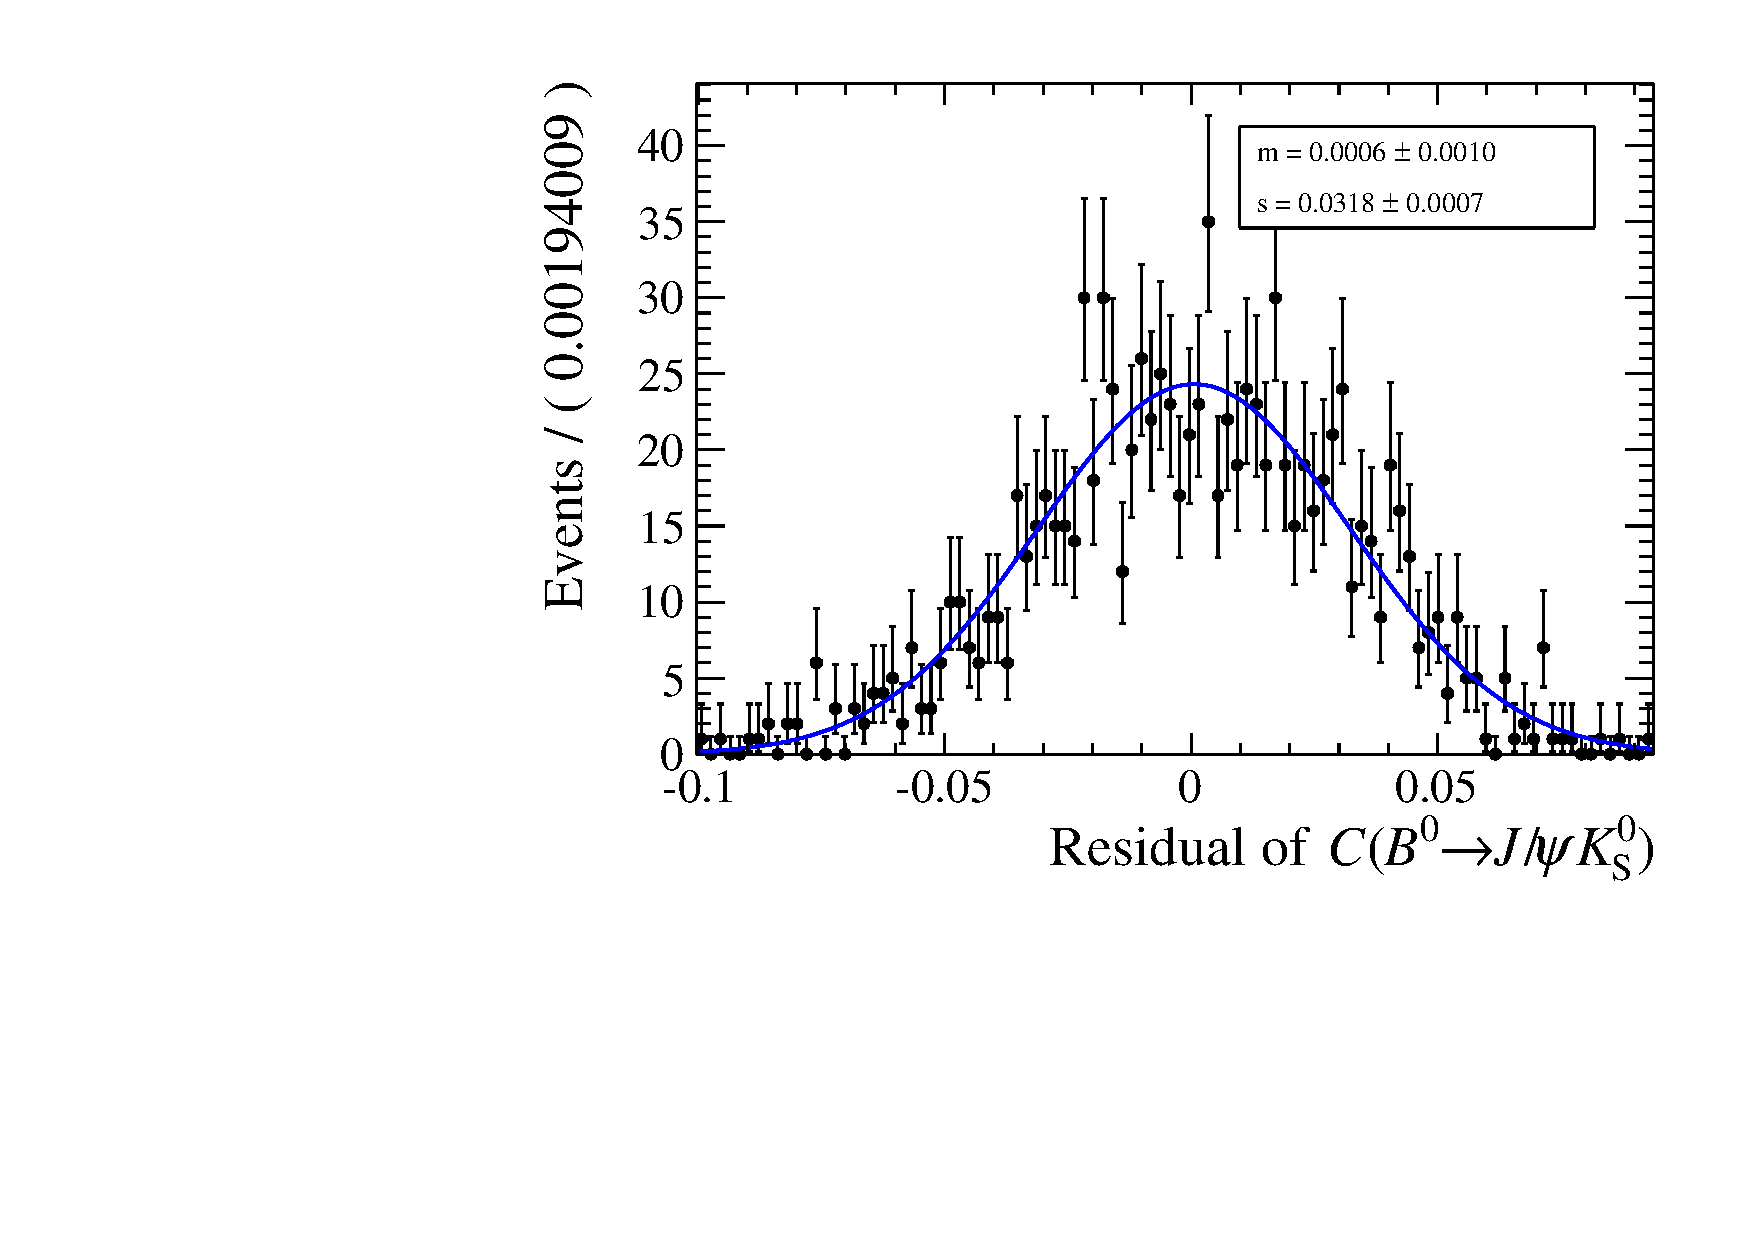
\includegraphics[width=0.49\textwidth]{private/content/appendices/figs/systematics_fs_prodasym_c_res.pdf}
\caption{Shown are (left) pull and (right) residual distributions of the
parameters (top) \SJpsiKS and (bottom) \CJpsiKS from a \ToyMC study of the
influence of an enlarged production asymmetry $A_P^{\catOO}$ on the measurement
of the \CP parameters.}
\label{fig:app:measurement_of_sin2beta:systematics:systematics:further_studies:production_asymmetry}
\end{figure}

\begin{figure}[h]
  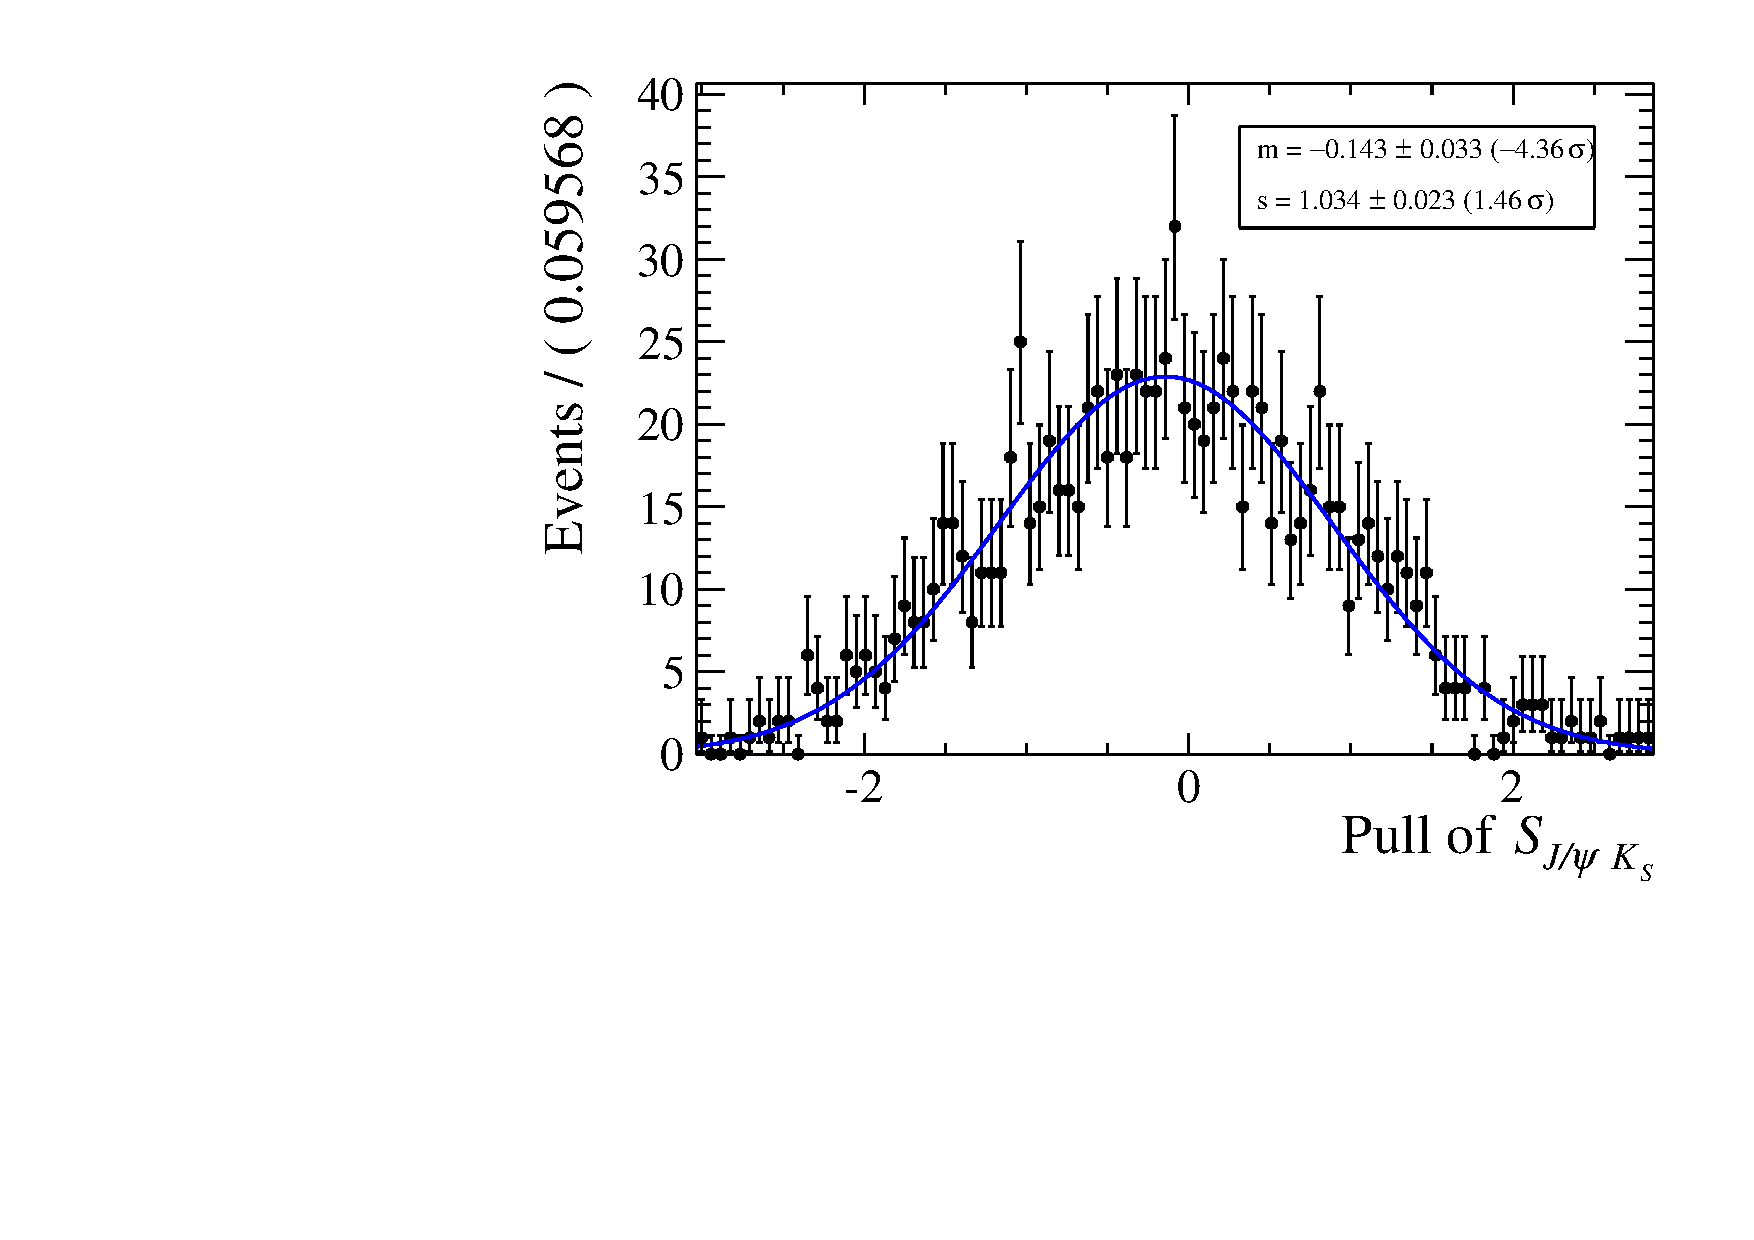
\includegraphics[width=0.49\textwidth]{private/content/appendices/figs/systematics_fs_dgd_s_pull.pdf}\hfill
  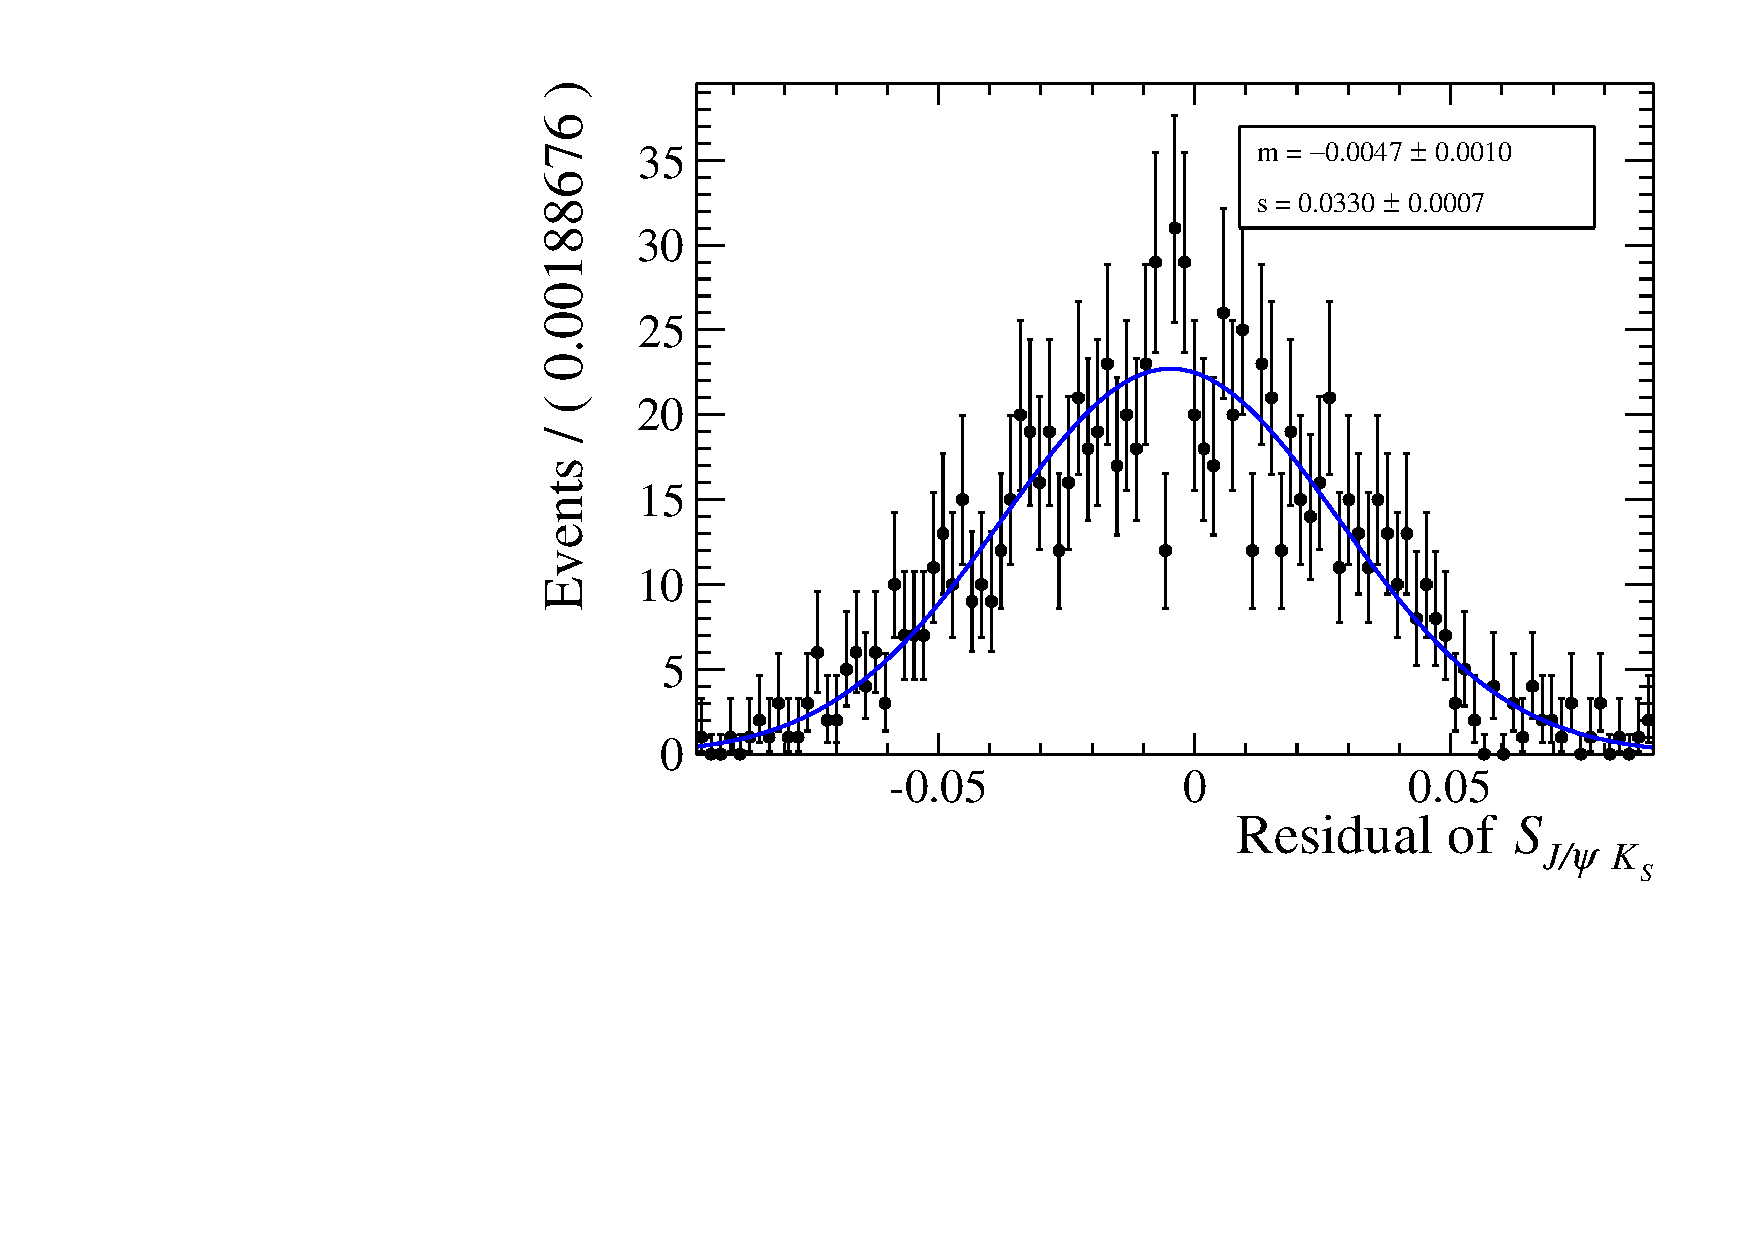
\includegraphics[width=0.49\textwidth]{private/content/appendices/figs/systematics_fs_dgd_s_res.pdf}
  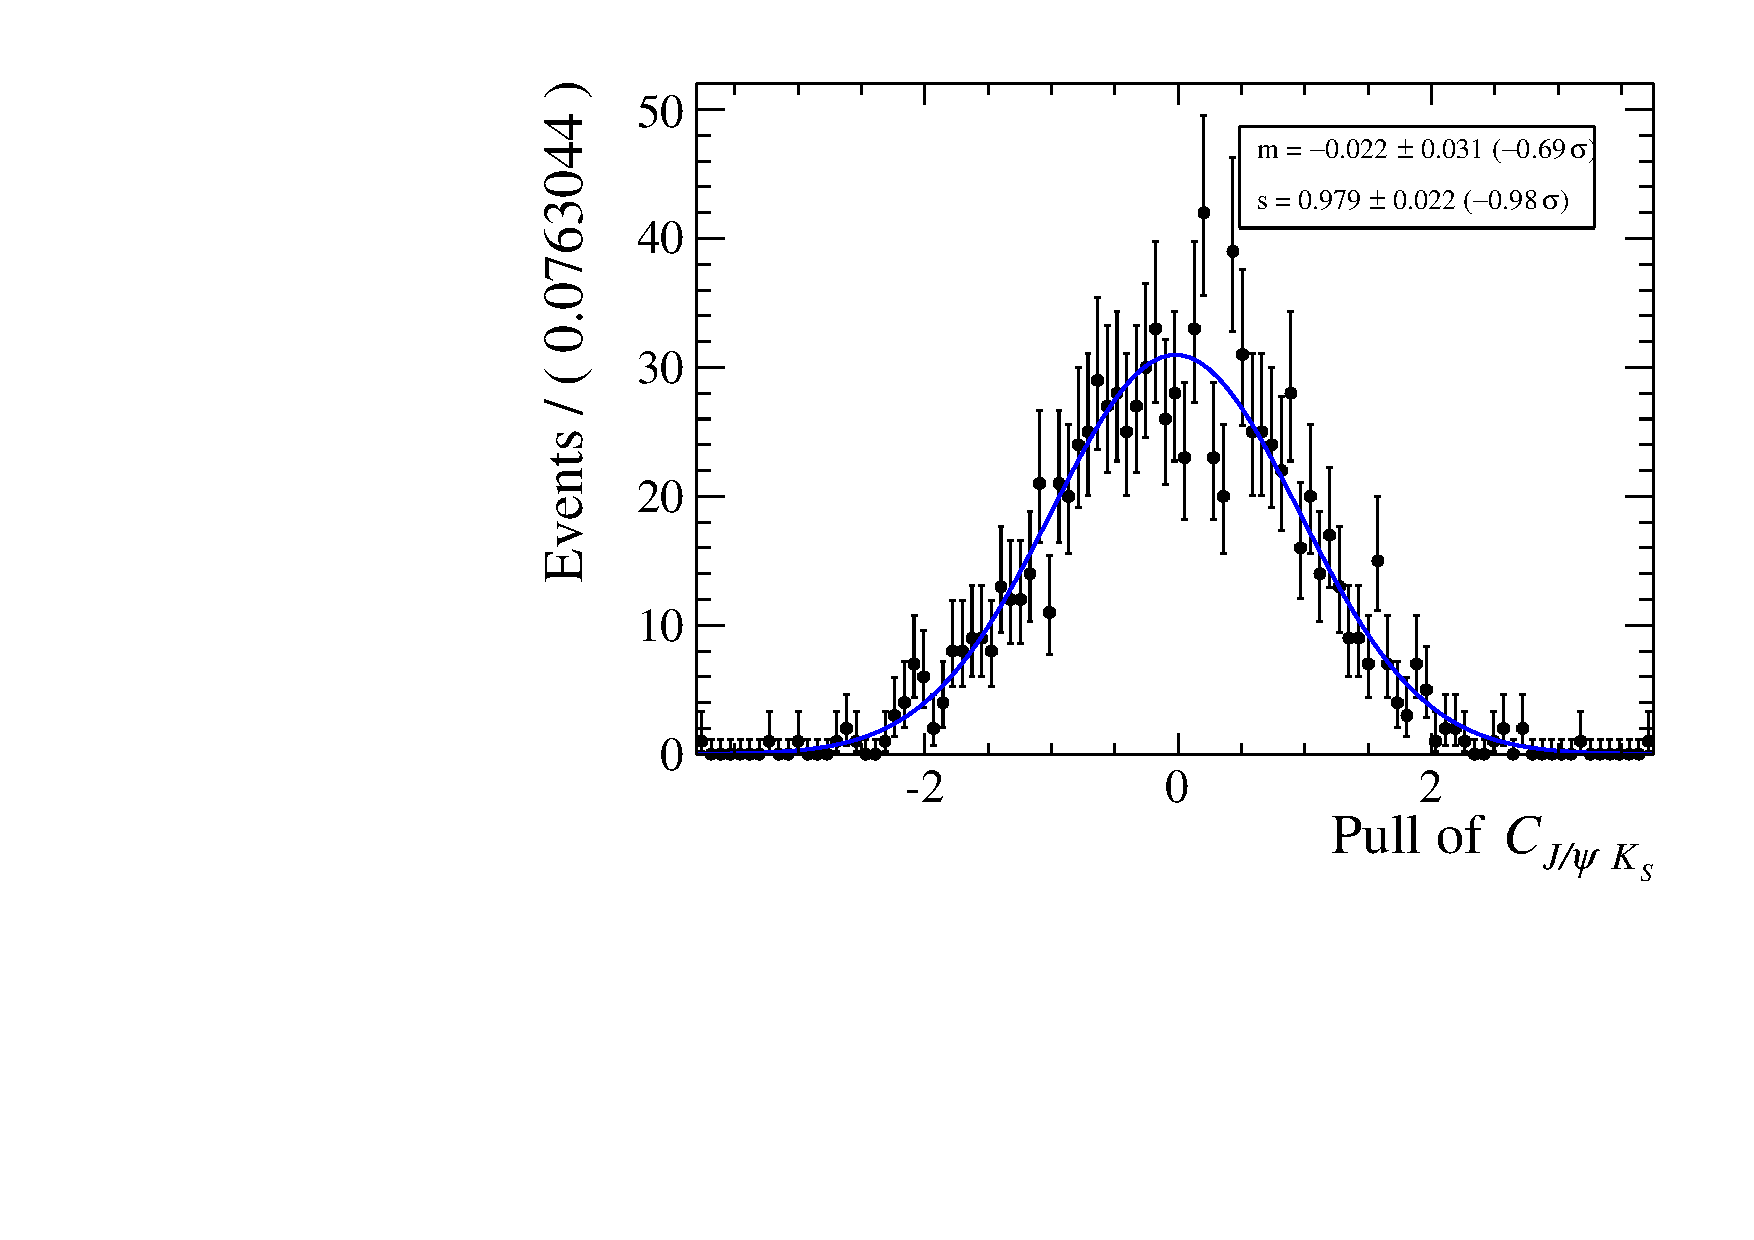
\includegraphics[width=0.49\textwidth]{private/content/appendices/figs/systematics_fs_dgd_c_pull.pdf}\hfill
  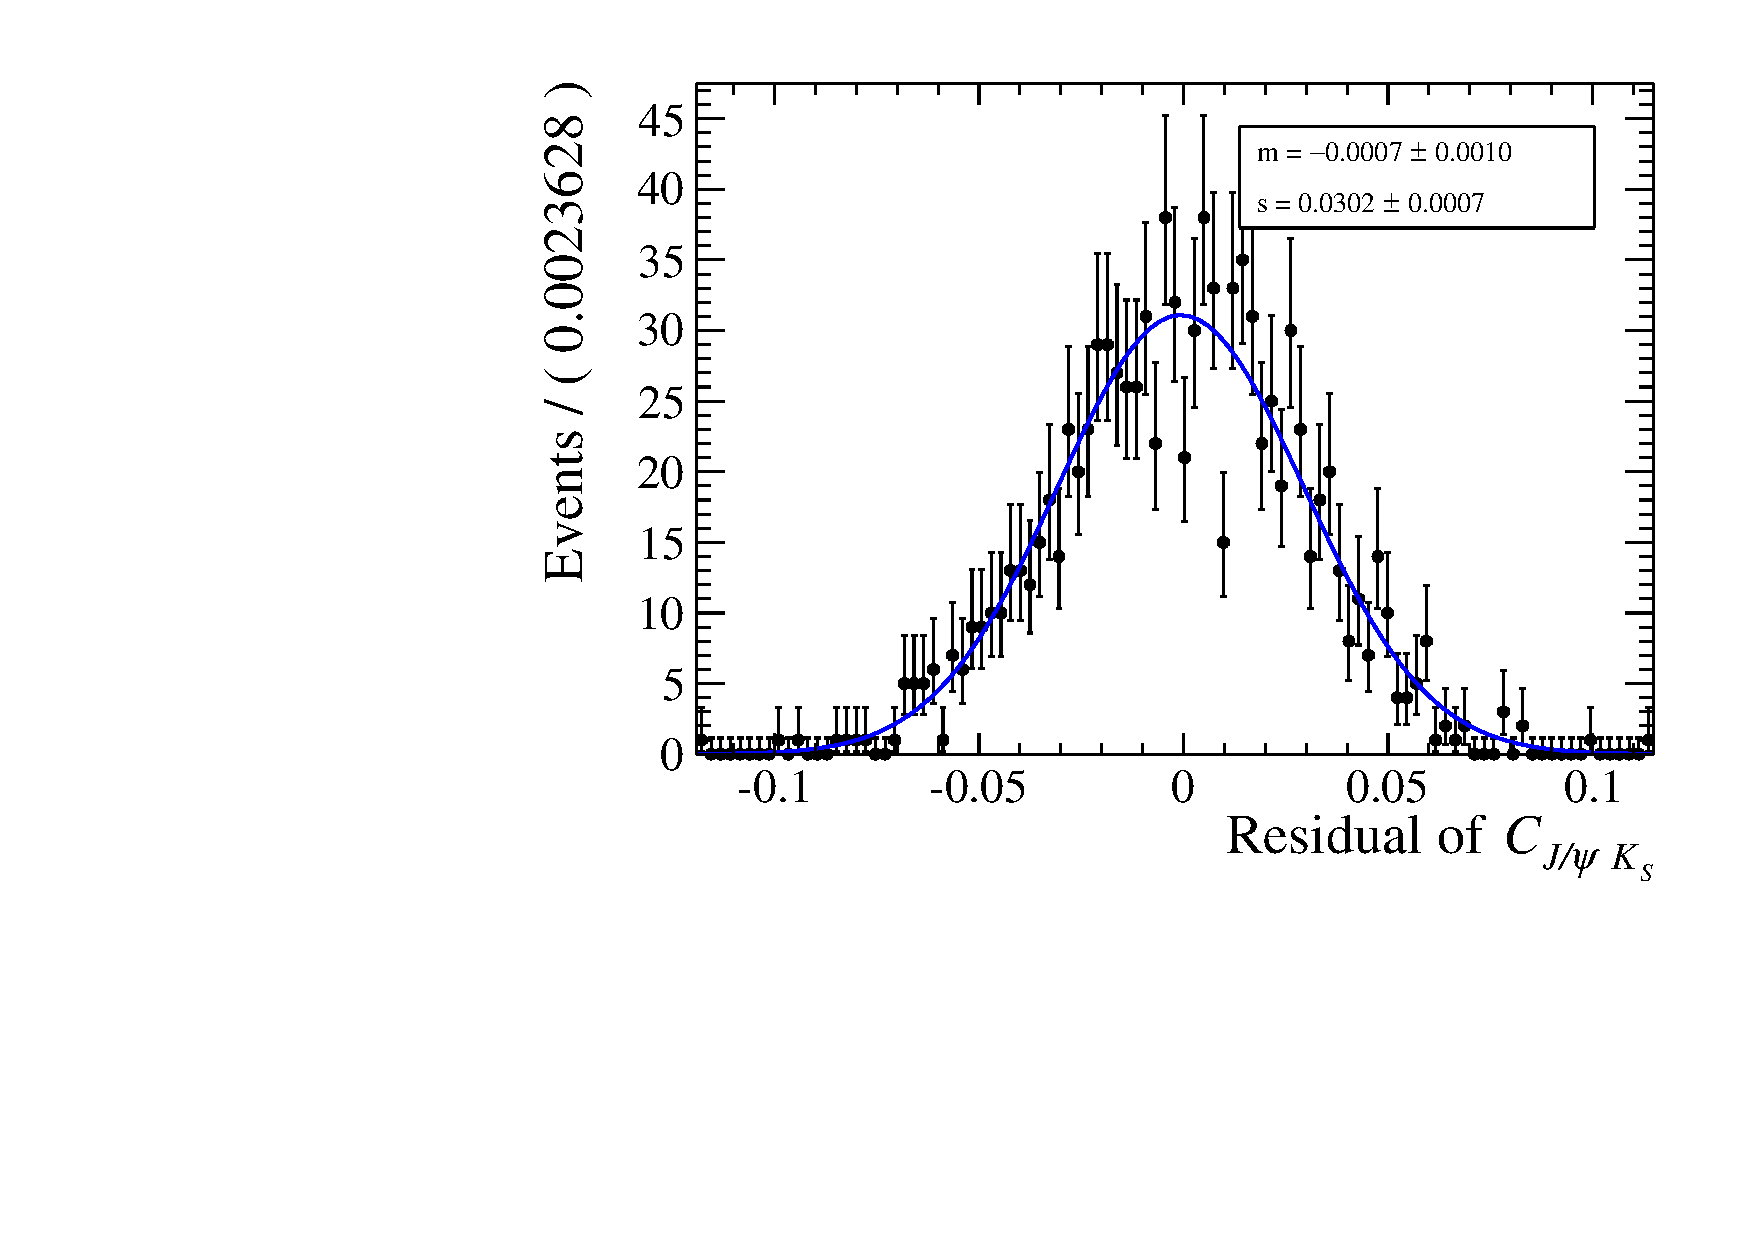
\includegraphics[width=0.49\textwidth]{private/content/appendices/figs/systematics_fs_dgd_c_res.pdf}
\caption{Shown are (left) pull and (right) residual distributions of the
parameters (top) \SJpsiKS and (bottom) \CJpsiKS from a \ToyMC study of the
influence of a non-zero decay width difference $\DGd$ on the measurement
of the \CP parameters.}
\label{fig:app:measurement_of_sin2beta:systematics:systematics:further_studies:decay_width_difference}
\end{figure}

\begin{figure}[h]
  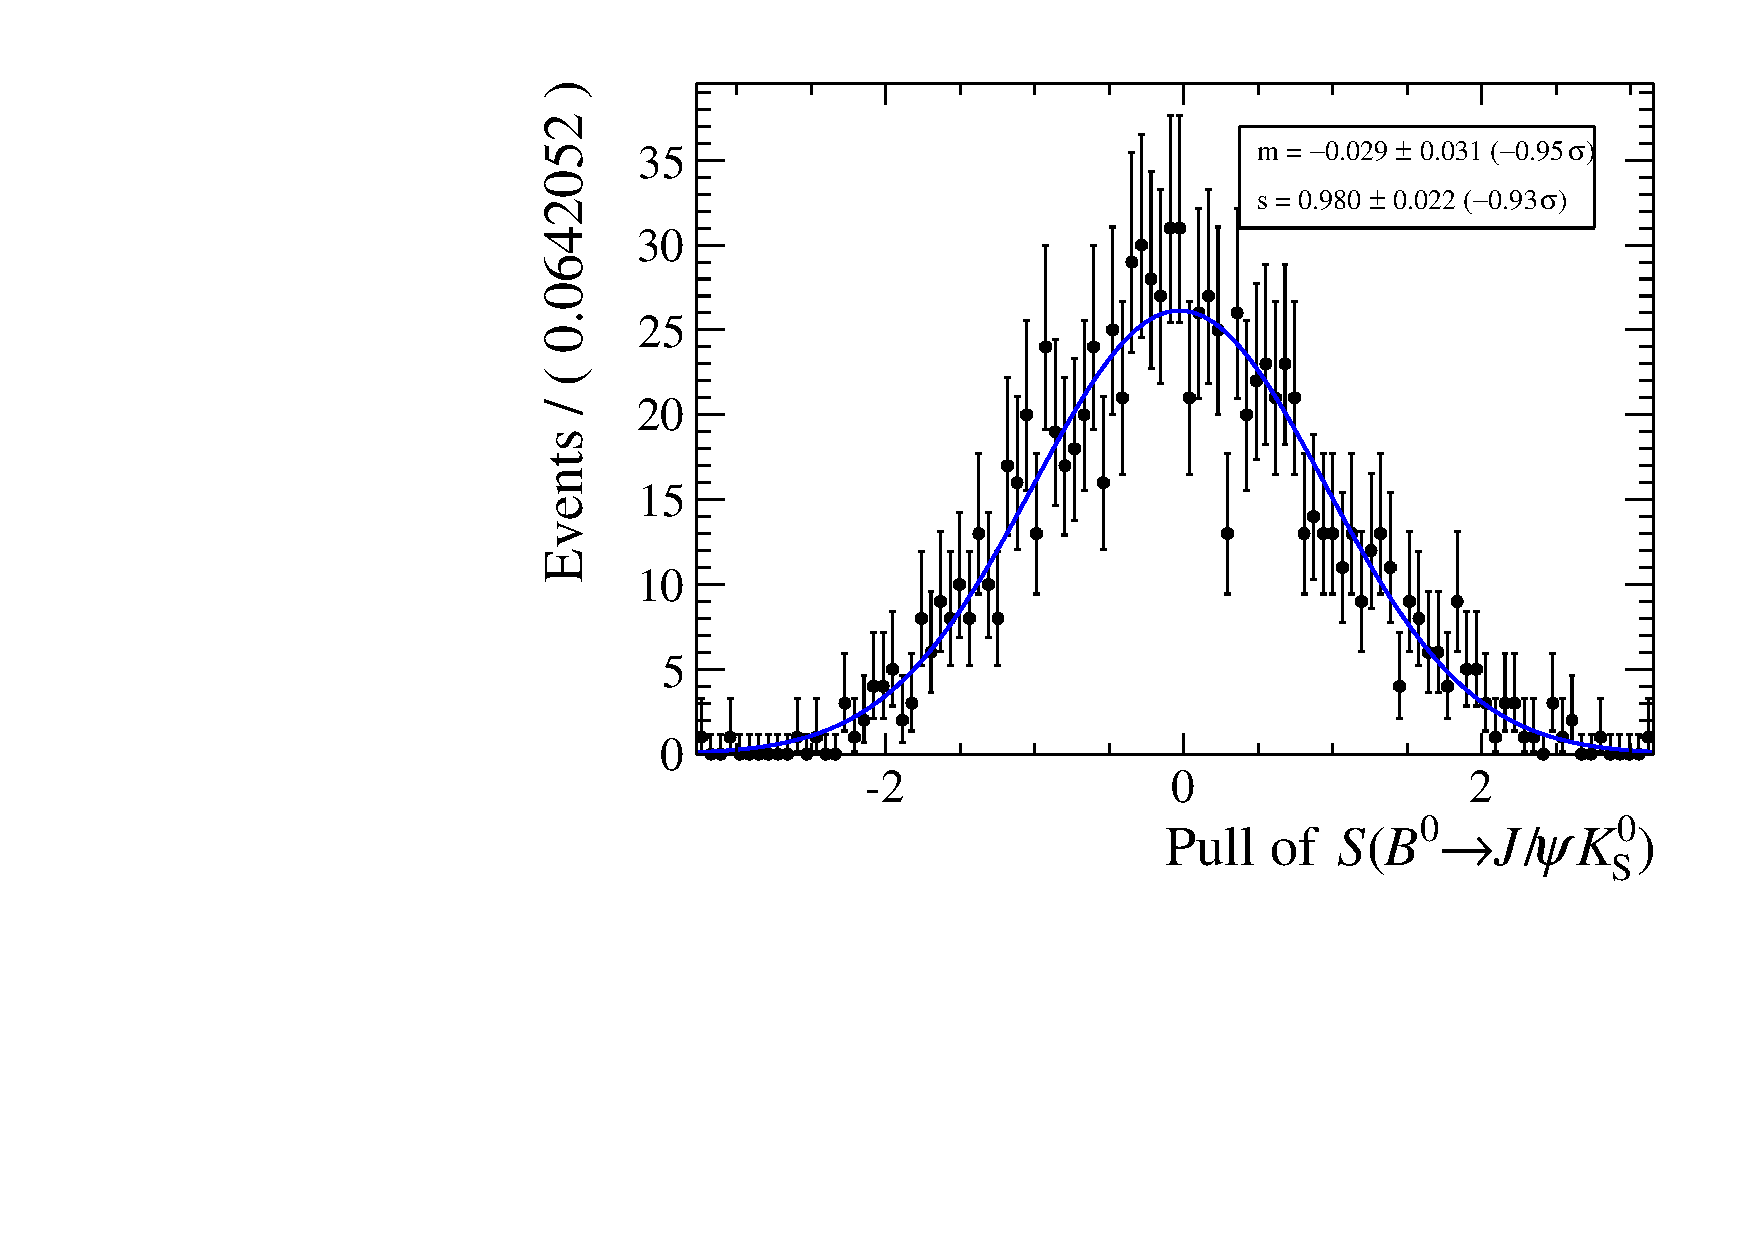
\includegraphics[width=0.49\textwidth]{private/content/appendices/figs/systematics_fs_dmd_s_pull.pdf}\hfill
  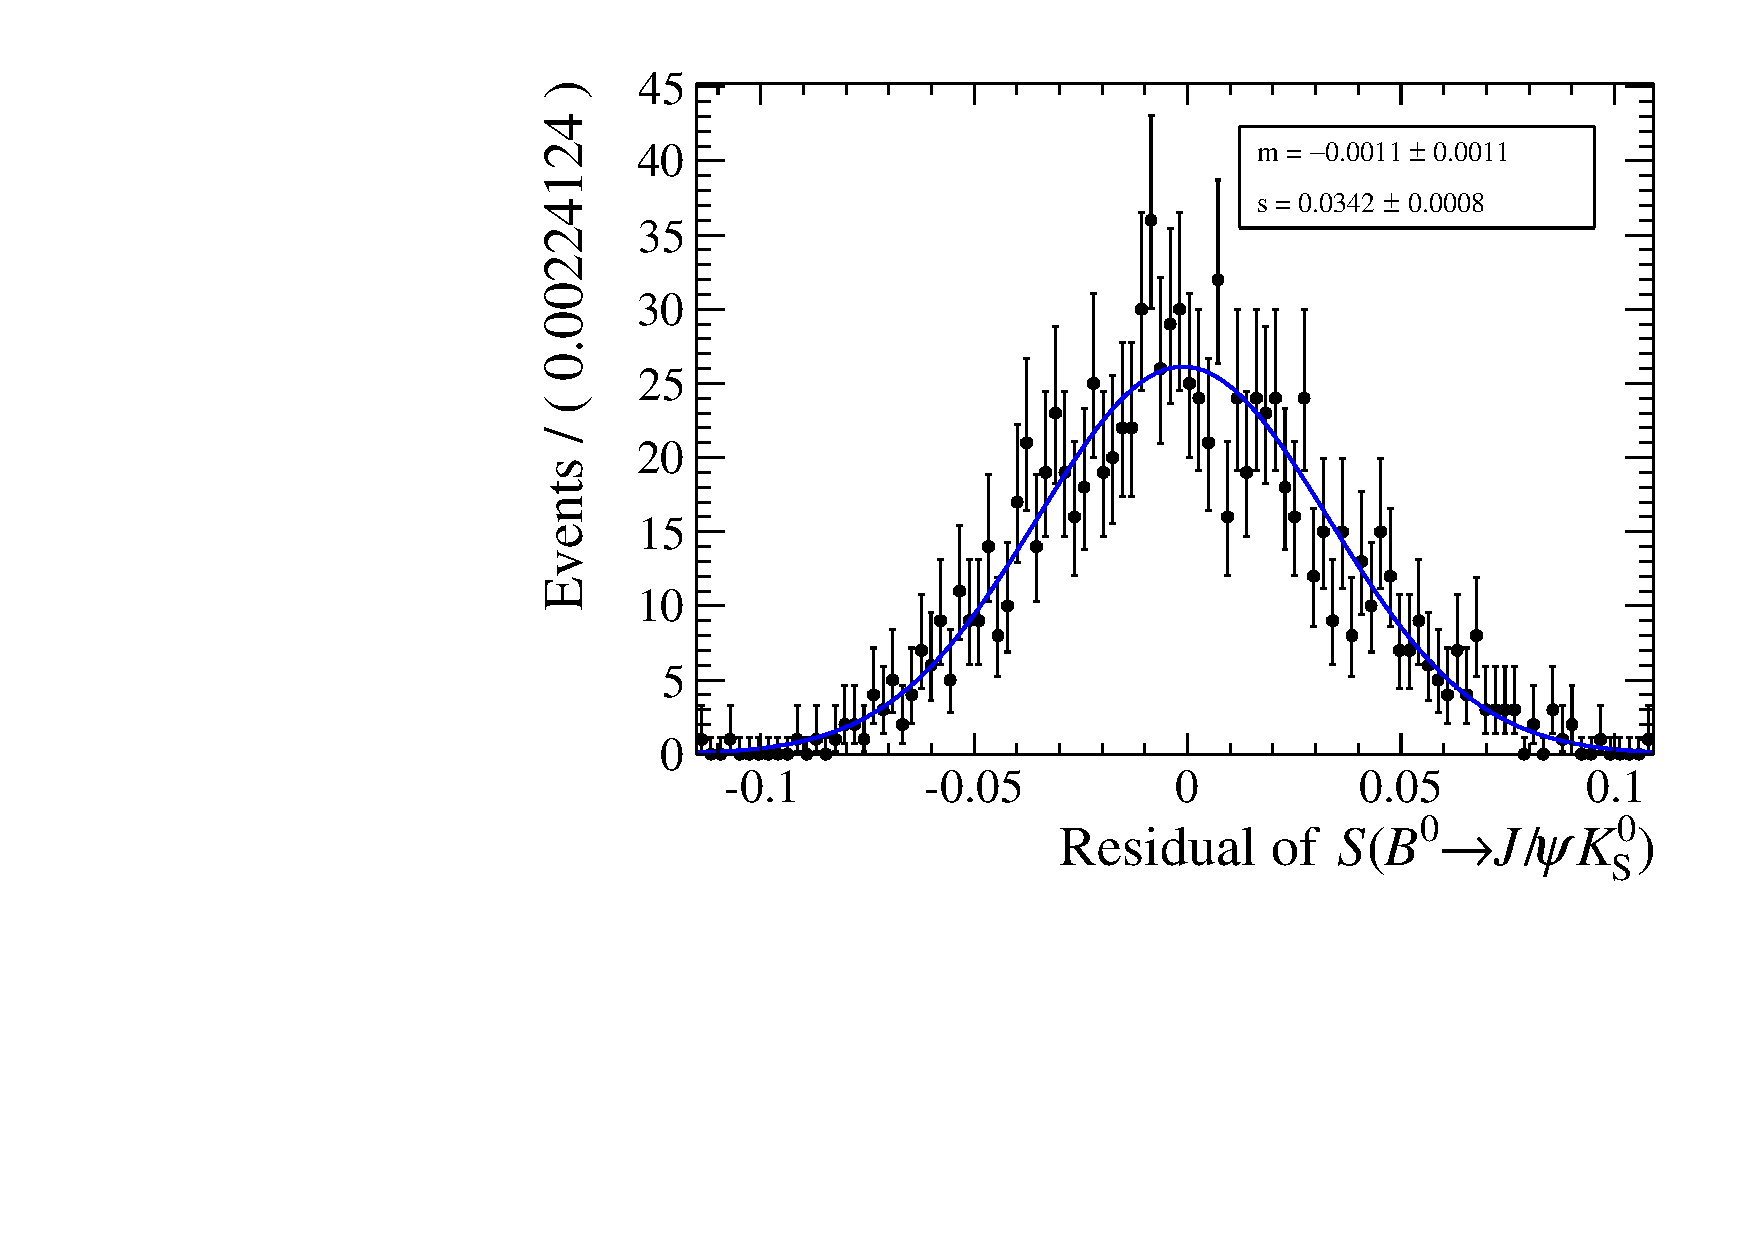
\includegraphics[width=0.49\textwidth]{private/content/appendices/figs/systematics_fs_dmd_s_res.pdf}
  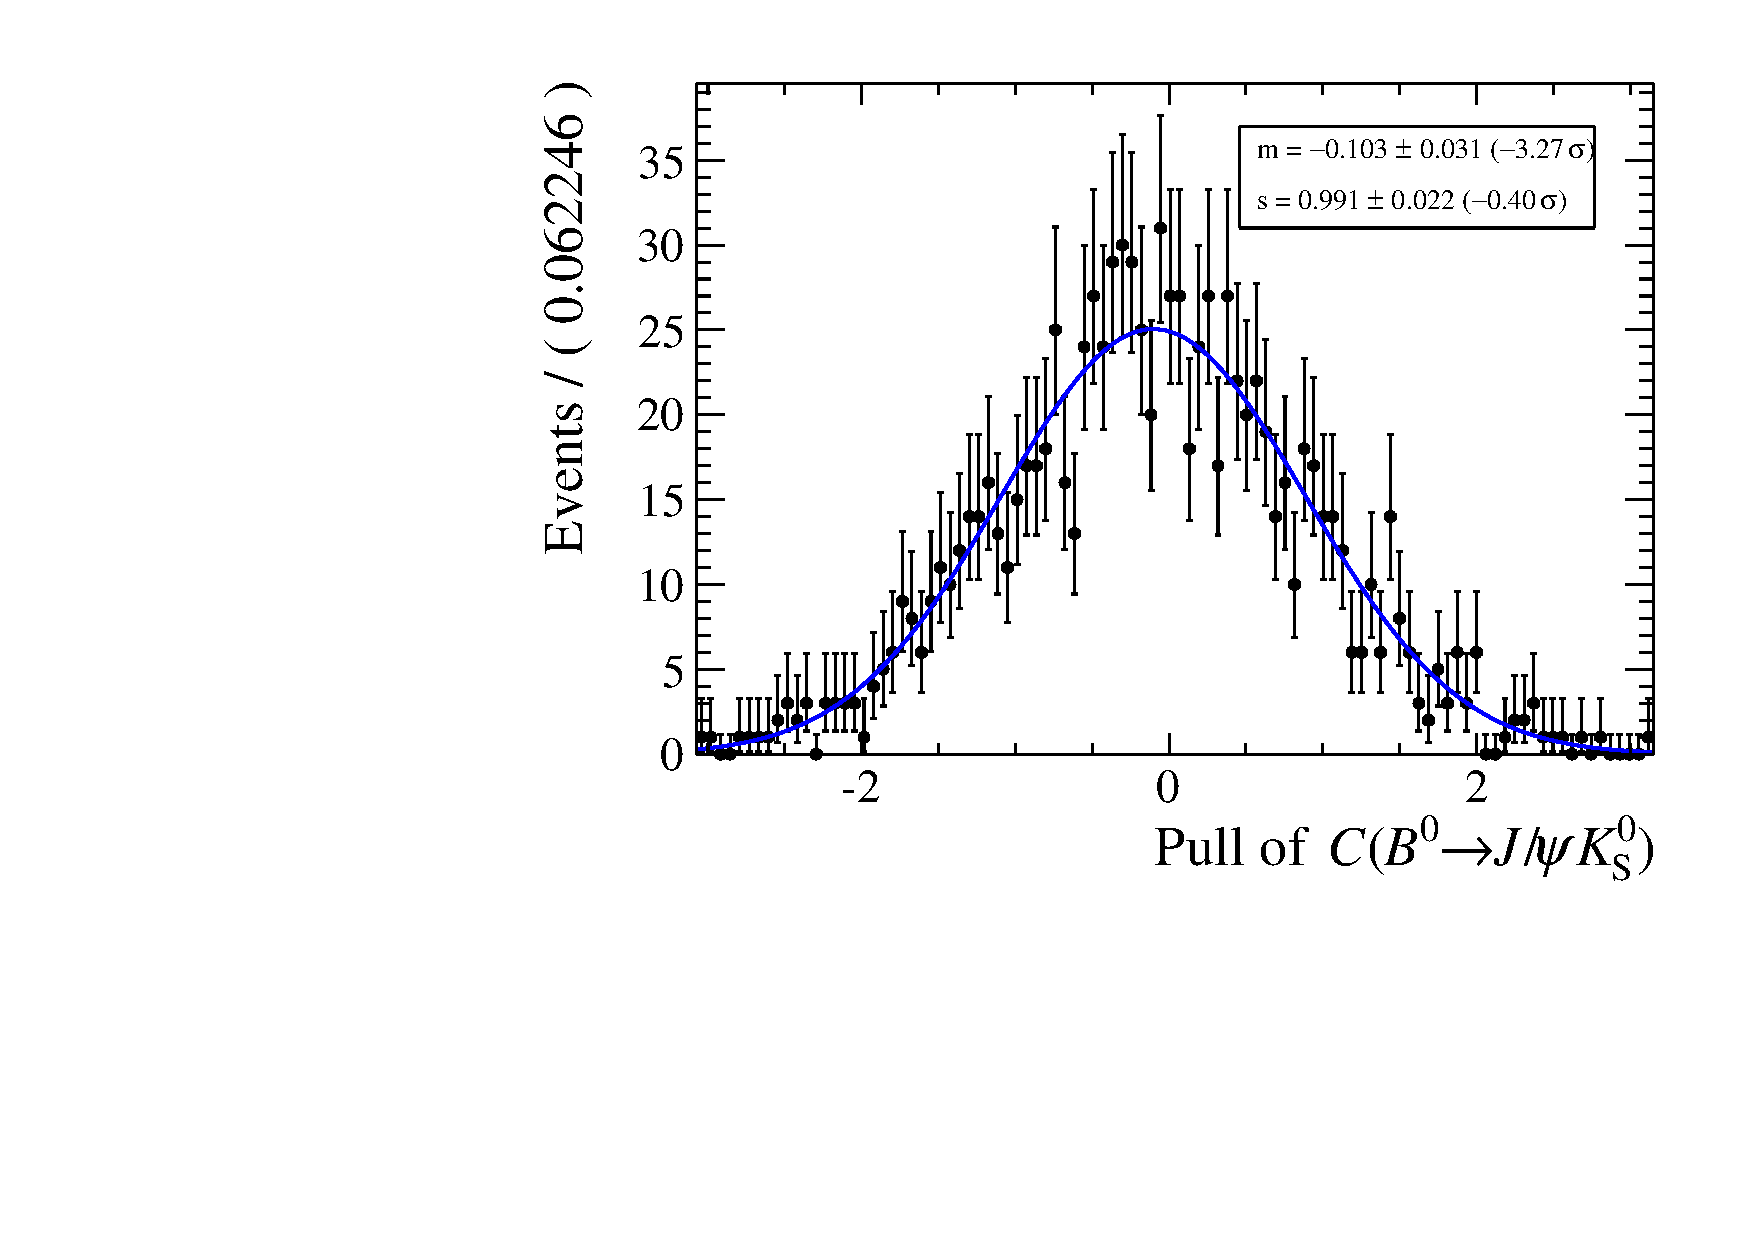
\includegraphics[width=0.49\textwidth]{private/content/appendices/figs/systematics_fs_dmd_c_pull.pdf}\hfill
  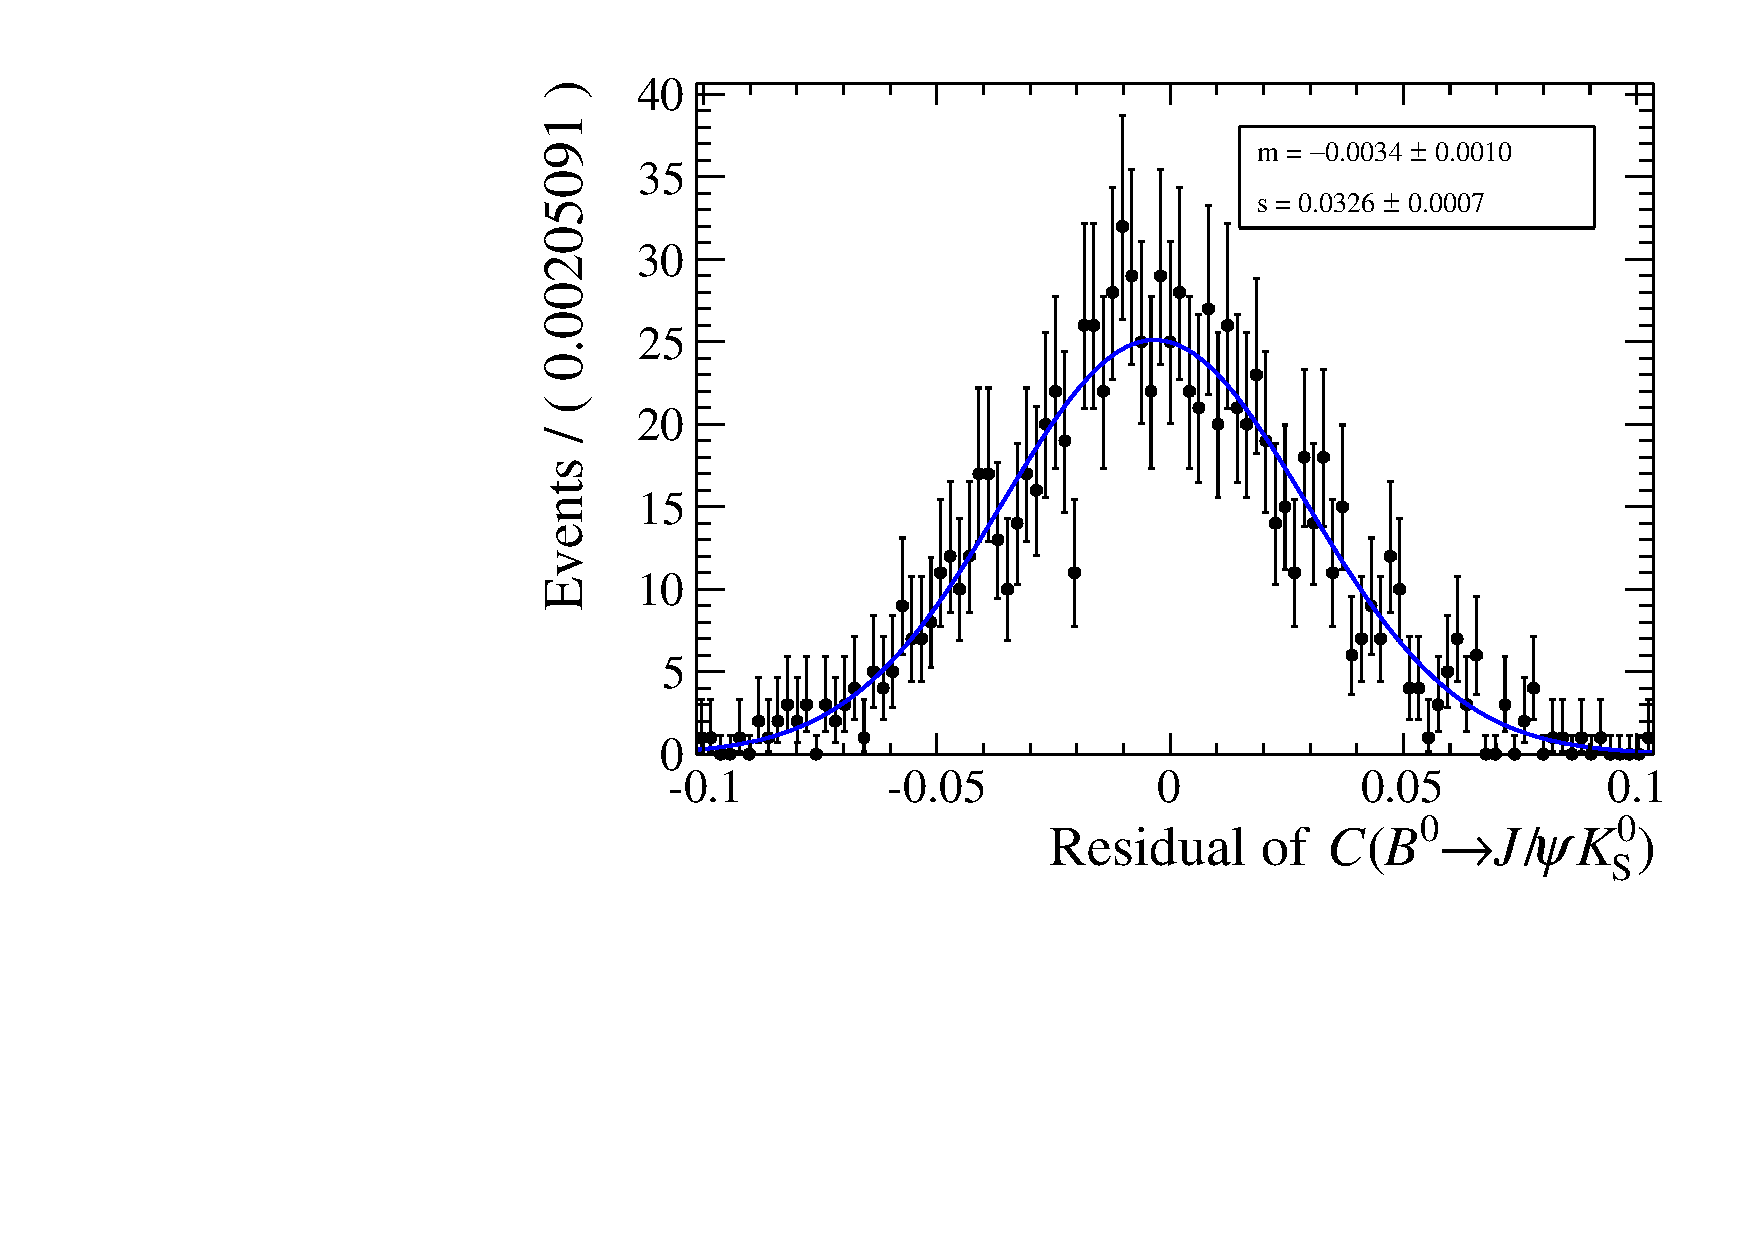
\includegraphics[width=0.49\textwidth]{private/content/appendices/figs/systematics_fs_dmd_c_res.pdf}
\caption{Shown are (left) pull and (right) residual distributions of the
parameters (top) \SJpsiKS and (bottom) \CJpsiKS from a \ToyMC study of the
influence of an enlarged mass difference $\DMd$ on the measurement
of the \CP parameters.}
\label{fig:app:measurement_of_sin2beta:systematics:systematics:further_studies:mass_difference}
\end{figure}
